\documentclass%
%[handout]
{beamer}
% % % % % % % %
% % % % % % % %
% % % % % % % %
%IMPORTANT
%compiles with 
%pdflatex -shell-escape 
%IMPORTANT
% % % % % % % %
% % % % % % % %
% % % % % % % %
\mode<presentation>
{
\useinnertheme{rounded}
\useoutertheme{infolines}
\usecolortheme{orchid}
\usecolortheme{whale}
}

\usepackage[english]{babel}
\usepackage[latin1]{inputenc}
\usepackage[all,cmtip]{xy}
\usepackage{times}
\usepackage[T1]{fontenc}
\usepackage{../example-templates}
\usepackage{../pstricks-commands}

\usepackage{auto-pst-pdf}
\usepackage{pst-plot}
%\usepackage{pstricks-add} 

% Or whatever. Note that the encoding and the font should match. If T1
% does not look nice, try deleting the line with the fontenc.


\graphicspath{{../../modules/}}

\newtheoremstyle{partialproof}{3pt}{3pt}{}{}{}{.}{.5em}{}
\theoremstyle{partialproof} \newtheorem{partialproof}[theorem]{Proof.}
%\DeclareMathOperator{\diff}{d}
\setbeamertemplate{navigation symbols}{}

\includeonlylecture{1}

\newcommand{\lect}[3]{
  \date{#1}
  \lecture[#1]{#2}{#3}
}

\setbeamertemplate{footline}
{
  \leavevmode%
  \hbox{%
  \begin{beamercolorbox}[wd=.333333\paperwidth,ht=2.25ex,dp=1ex,center]{author in head/foot}%
    \usebeamerfont{author in head/foot}\insertshortauthor
  \end{beamercolorbox}%
  \begin{beamercolorbox}[wd=.333333\paperwidth,ht=2.25ex,dp=1ex,center]{title in head/foot}%
    \usebeamerfont{title in head/foot}\insertshorttitle
  \end{beamercolorbox}%
  \begin{beamercolorbox}[wd=.333333\paperwidth,ht=2.25ex,dp=1ex,center]{date in head/foot}%
    \usebeamerfont{date in head/foot}\insertshortdate{}
  \end{beamercolorbox}}%
  \vskip0pt%
}

% If you have a file called "university-logo-filename.xxx", where xxx
% is a graphic format that can be processed by latex or pdflatex,
% resp., then you can add a logo as follows:

%\pgfdeclareimage[height=0.8cm]{logo}{bluelogo}
%\logo{\pgfuseimage{logo}}
\renewcommand{\Arcsin}{\arcsin}
\renewcommand{\Arccos}{\arccos}
\renewcommand{\Arccot}{\text{arccot}}
\renewcommand{\Arctan}{\arctan}

\begin{document}

\AtBeginLecture{%

\title[\insertlecture]{FreeCalc}
\subtitle{\insertlecture}
\author[FreeCalc]{}
\institute[UMass Boston]{University of Massachusetts Boston}
\date{\insertshortlecture}
\begin{frame}
  \titlepage
\end{frame}
}%

% begin lecture
\lect{\today}{Sample}{1}
% begin module polar-area-justification
\begin{frame}[t]
\begin{columns}
\frametitle{Area swept by a polar curve: justification}
\column{0.5\textwidth}
\psset{xunit=1cm, yunit=1cm, algebraic=false}
\begin{pspicture}(-2.65,-1)(1.4,2.3)%
\tiny%
\psline[linecolor=red!1](1.4, 2.3)(1.39, 2.3)%
\psline[linecolor=red!1](-2.65, -1)(-2.649, -1)%
\rput[t](0,-0.1){$O$}%
\pstVerb{%
10 dict begin
/thePolarR {t 2 div 1 add} def
/thePolarX {t 57.295779513 mul cos thePolarR mul} def
/thePolarY {t 57.295779513 mul sin thePolarR mul} def
/thetaMax 3.5 def
}%
\uncover<1>{%
\pscustom*[linecolor=cyan]{%
\fcDrawPolar[linecolor=red, plotpoints=1000]{0}{thetaMax}{thePolarR}%
\pstVerb{1 dict begin /t thetaMax def}%
\psline(! thePolarX thePolarY )(0,0)(1,0)%
\pstVerb{end}%
}%
\pstVerb{1 dict begin /t thetaMax def}%
\psline[linecolor=red](! thePolarX thePolarY )(0,0)(1,0)%
\pstVerb{end}%
}%
\rput[t](1.2,-0.1){$x$}%
\uncover<2-15>{%
\rput[b](-0.832294, 1.85){$\alertNoH{4}{P_2}$}%
\rput[bl](0.84, 1.3){$\alertNoH{4}{P_1}$}%
\pstVerb{1 dict begin /t 1 def}%
\fcFullDot{thePolarX}{thePolarY}%
\pstVerb{/t 2 def}%
\fcFullDot{thePolarX}{thePolarY}%
\pstVerb{end}%
}%
\uncover<5-15>{%
\pstVerb{1 dict begin /t 1 def}%
\psline[linecolor=cyan](0,0)(! thePolarX thePolarY)%
\pstVerb{/t 2 def}%
\psline[linecolor=cyan](0,0)(! thePolarX thePolarY)%
\pstVerb{end}%
}%
\uncover<7-15>{%
\fcPolarWedge{1}{2}{thePolarR}%
}%
\uncover<8,9,10>{%
\pstVerb{1 dict begin /t 1 def}%
\psline[linecolor=red, linewidth=2pt](0,0)(! thePolarX thePolarY)%
\pstVerb{/t 2 def}%
\psline[linecolor=red, linewidth=2pt](0,0)(! thePolarX thePolarY)%
\pstVerb{end}%
}%
\uncover<5-15>{%
\rput[bl](0.50, 0.6){$r_1$}%
\rput[l](-0.45, 1.1){$r_2$}%
}%
\uncover<6-15>{%
\fcAngle{1}{2}{0.7}{}%
\fcAngle{0}{2}{0.45}{}%
\fcAngle{0}{1}{0.15}{}%
\rput[bl](0.15, 0.05){$\alertNoH{6}{\theta_1}$}%
\rput[b](0, 0.46){$\alertNoH{6}{\theta_2}$}%
\rput[b](0, 0.73){$ \alertNoH{9,10}{\Delta}$}%
}%
\uncover<handout:2|11-15>{%
\fcPolarWedgeSequence{0}{1}{3}{thePolarR}%
}%
\uncover<handout:2|16>{%
\fcPolarWedgeSequence{0}{0.75}{4}{thePolarR}%
}%
\uncover<handout:2|17>{%
\fcPolarWedgeSequence{0}{0.5}{6}{thePolarR}%
}%
\uncover<handout:2|18>{%
\fcPolarWedgeSequence{0}{0.3}{10}{thePolarR}%
}%
\uncover<handout:2|19>{%
\fcPolarWedgeSequence{0}{0.2}{15}{thePolarR}%
}%
\uncover<handout:2|20->{%
\fcPolarWedgeSequence{0}{0.1}{30}{thePolarR}%
}%
\fcDrawPolar[linecolor=red, plotpoints=1000]{0}{3.5}{thePolarR}%
\psline[arrows=->](0,0)(1.2, 0)%
\pstVerb{end}%
\end{pspicture}

\column{0.5\textwidth}
\uncover<2->{Split $[a,b]$ into $N$ equal segments via points $a=\theta_0 \leq \theta_1 \leq \dots \leq \theta_{N-1} \leq \theta_N=b$.} \uncover<3->{The length of each segment is $\Delta=\frac{b-a}{N}$.} \uncover<4->{Let $r_i=f(\theta_i)$. Then each $\theta_i$ gives a \alertNoH{4}{point $P_i$} with polar coordinates $(\alertNoH{5}{r_i},\alertNoH{6}{\theta_i})$.}
\end{columns}

\only<handout:1|1-12>{ \uncover<7->{The area swept by the curve is approximated by sum of areas of triangles given by connecting the origin with two consecutive vertices. Consider one such triangle, say, $OP_1P_2$.} \uncover<8->{By Euclidean geometry, the area of $\triangle OP_1P_2 $ is $\alertNoH{8,9}{\frac{|OP_1| |OP_2|  \fcAnswer{9}{ \sin \Delta}}{2}} \uncover<10->{=\frac{ r_1 r_2 \sin \Delta}{2}= \frac{ f(\theta_1) f(\theta_2) \sin \Delta}{2}} $.}
}

\uncover<handout:2| 11->{\alertNoH{12,13}{ Therefore the area swept by the curve \only<handout:0|1-14>{is approximated by} \only<handout:2|15->{\alertNoH{15}{equals \alertNoH{16-}{the limit} of}} the sum:}
\[\begin{array}{rcl}
\uncover<15->{ A&=&}\alertNoH{12,13}{\uncover<15->{\lim\limits_{\Delta\to 0}} \sum\limits_{i=0}^{N-1} \frac{f(\theta_i)f(\theta_{i+1}) \alertNoH{14}{ \sin \Delta} }{2}} \uncover<14->{= \uncover<15->{ \lim \limits_{\Delta\to 0}} \alertNoH{14}{ \frac{ \sin\Delta}{ \Delta}} \sum\limits_{i=0}^{N-1} \frac{ f( \theta_i) f(\theta_{i} + \Delta)\alertNoH{14}{\Delta}}{2}}\\
\uncover<21->{\uncover<24>{\alertNoH{24}{\text{{\tiny(can be proved)}}}}  &=&   \alertNoH{22,23}{ \lim \limits_{\Delta\to 0}\frac{ \sin\Delta}{ \Delta  }}  \lim \limits_{\alertNoH{24}{\Delta\to 0} } \sum\limits_{i=0}^{N-1} \frac{ f( \theta_i) f( \alertNoH{24}{ \theta_{i} + \Delta} )\Delta}{2} \uncover<22->{=  \fcAnswer{23}{1}\cdot \lim \limits_{\Delta\to 0} \sum\limits_{i=0}^{N-1} \frac{\alertNoH{25}{ f( \theta_i) f(\alertNoH{24}{ \theta_{i}} )} \Delta}{2}}} \\
\uncover<25->{\uncover<27->{{\tiny\text{\alertNoH{27}{(Riemann sum)}}}} &=& \lim \limits_{\Delta\to 0} \sum \limits_{i=0}^{N-1} \frac{ \alertNoH{25}{ f^2( \theta_i)}  \Delta }{2}}\uncover<26->{=  \fcAnswer{27}{  \int\limits_{a}^b \frac{ f^2(\theta)}{2}\diff \theta} }
\end{array}
\]
}
\end{frame}
%end module polar-area-justification



%%begin module graphs-of-functions-as-curves
\begin{frame}
\frametitle{Graphs of functions as curve images}
\begin{itemize}
\item Consider a graph of a function given by 
\[
y=f(x)
\]
\item<2-> Write $\alert<3>{x=t}$. Then $y=f(x)\uncover<3->{ =f(\alert<3>{t})}$\uncover<4->{, so we get the system }
\uncover<4->{
\[
C: \left|\begin{array}{rcl}
x&=&t\\
y&=&f(t)
\end{array}\right., t\in [a,b]
\]
}
\end{itemize}
\uncover<5->{
\begin{observation}
The graph of an arbitrary function can be written as the image of a curve $C$ using the above transformation.
\end{observation}
}
\end{frame}

%end module graphs-of-functions-as-curves


%% begin module parametric-intro
\begin{frame}
\frametitle{Curves Defined by Parametric Equations}
\begin{columns}[c]
\column{.4\textwidth}

\psset{xunit=1cm, yunit=1cm}
\begin{pspicture}(-1.000000, -5)(1.500000,5) 
\psframe*[linecolor=white](-1.000000,-5)(1.500000,5) 
\tiny 
\psaxesStandard{-2}{-0.5}{2}{3.5}
%Calculator input: plotCurve{}(\cos{}(t^{2}), t \sin{}t+\sin{}t, 0, 3)
\parametricplot[arrows=->, linecolor=\psColorGraph, plotpoints=500] {0}{0.75}{t 2 exp 57.29578 mul cos t 57.29578 mul sin t 57.29578 mul sin t mul add }
\parametricplot[arrows=->, linecolor=\psColorGraph, plotpoints=500] {0.75}{1.5}{t 2 exp 57.29578 mul cos t 57.29578 mul sin t 57.29578 mul sin t mul add }
\parametricplot[arrows=->, linecolor=\psColorGraph, plotpoints=500] {1.5}{2.25}{t 2 exp 57.29578 mul cos t 57.29578 mul sin t 57.29578 mul sin t mul add }
\parametricplot[linecolor=\psColorGraph, plotpoints=500] {2.25}{3}{t 2 exp 57.29578 mul cos t 57.29578 mul sin t 57.29578 mul sin t mul add }

\uncover<1>{\psFullDot{0.987227}{ 0.545186} } 
\uncover<2>{\psFullDot{0.689498}{ 1.488321} }
\uncover<3>{\psFullDot{-0.379452}{ 2.365079}}
\uncover<4>{\psFullDot{-0.892288}{ 2.744270}}
\uncover<5->{\psFullDot{0.866232}{ 2.296575} }
\uncover<6->{
\rput[l](0.89,2.396575){$\begin{array}{l}(x,y)\uncover<7->{= (g(t), f(t))} \\\phantom{(x,y)}\uncover<8->{=(x(t), y(t))}\end{array}$}
}
\end{pspicture} 
%\ \only<handout:0| -1>{%
%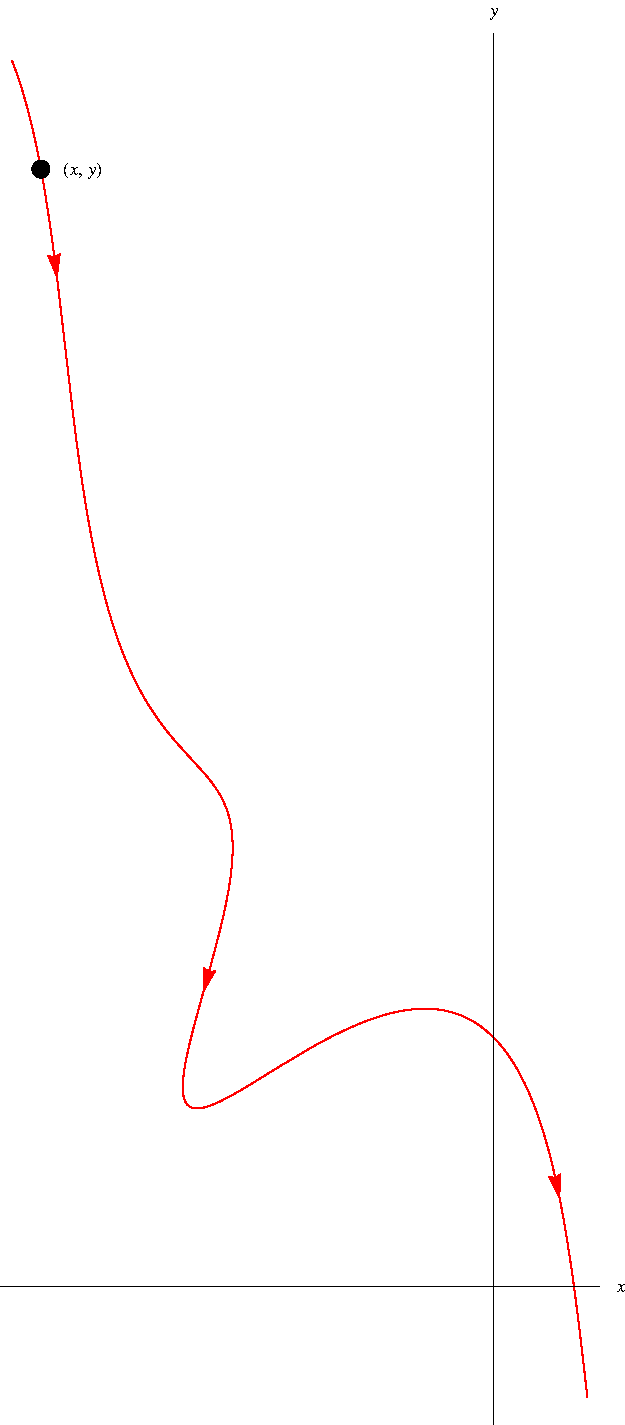
\includegraphics[height=7cm]{parametric-curves/pictures/11-01-parametrica.pdf}%
%}%
%\only<handout:0| 2>{%
%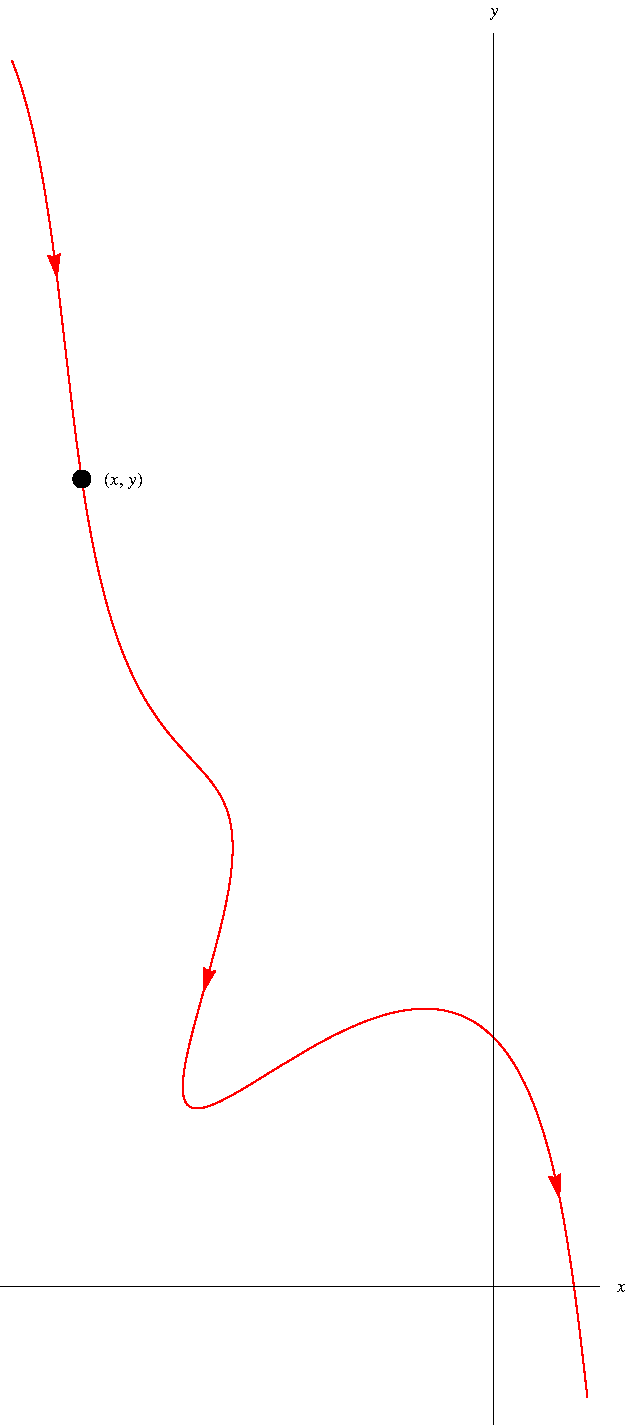
\includegraphics[height=7cm]{parametric-curves/pictures/11-01-parametricb.pdf}%
%}%
%\only<handout:0| 3>{%
%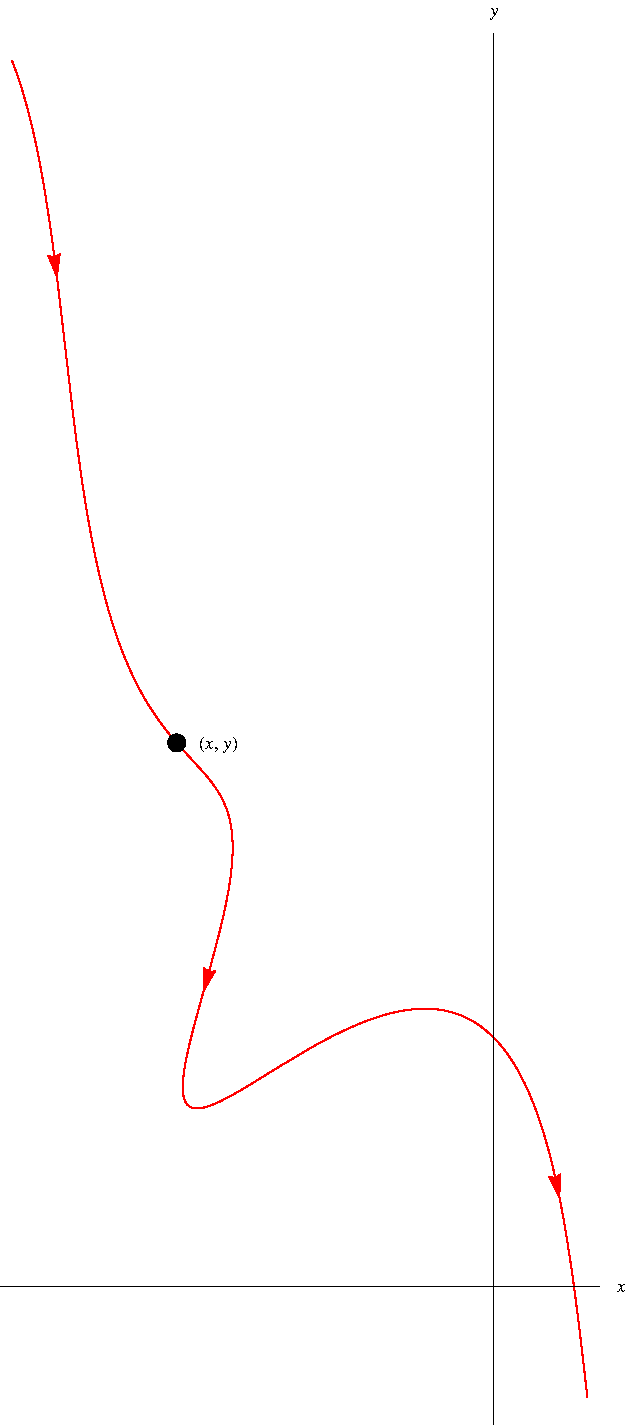
\includegraphics[height=7cm]{parametric-curves/pictures/11-01-parametricc.pdf}%
%}%
%\only<handout:0| 4>{%
%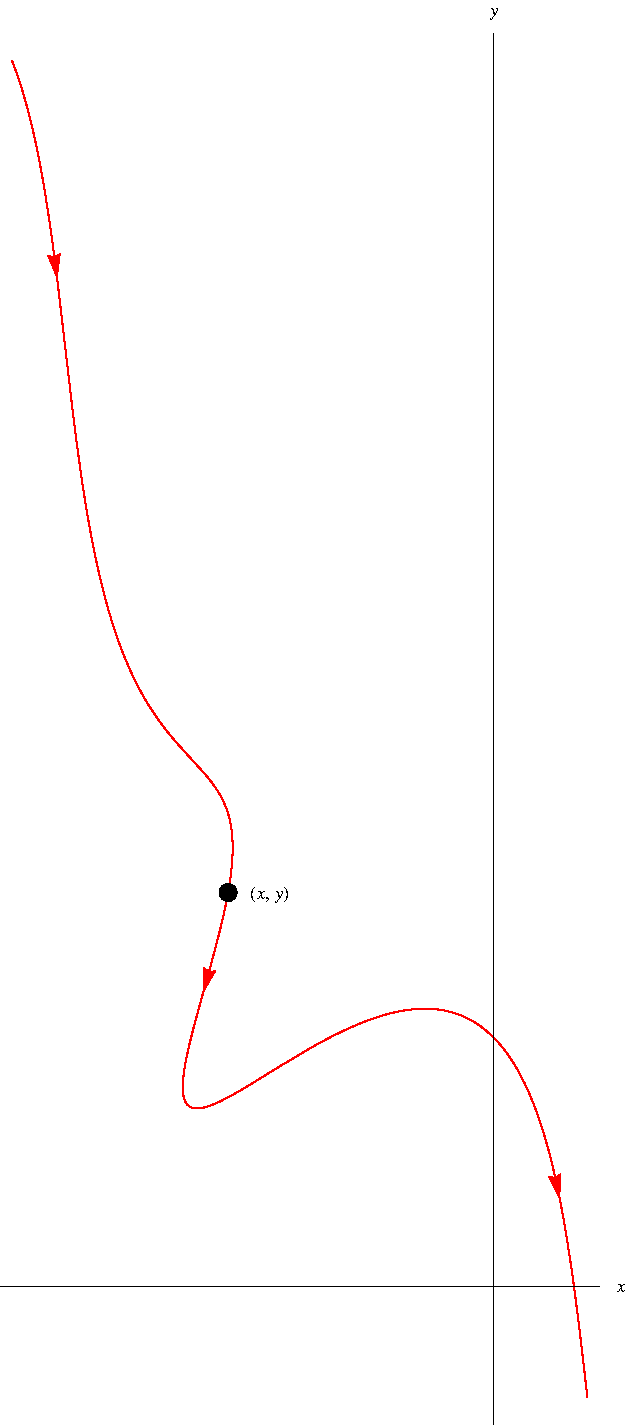
\includegraphics[height=7cm]{parametric-curves/pictures/11-01-parametricd.pdf}%
%}%
%\only<handout:0| 5-7>{%
%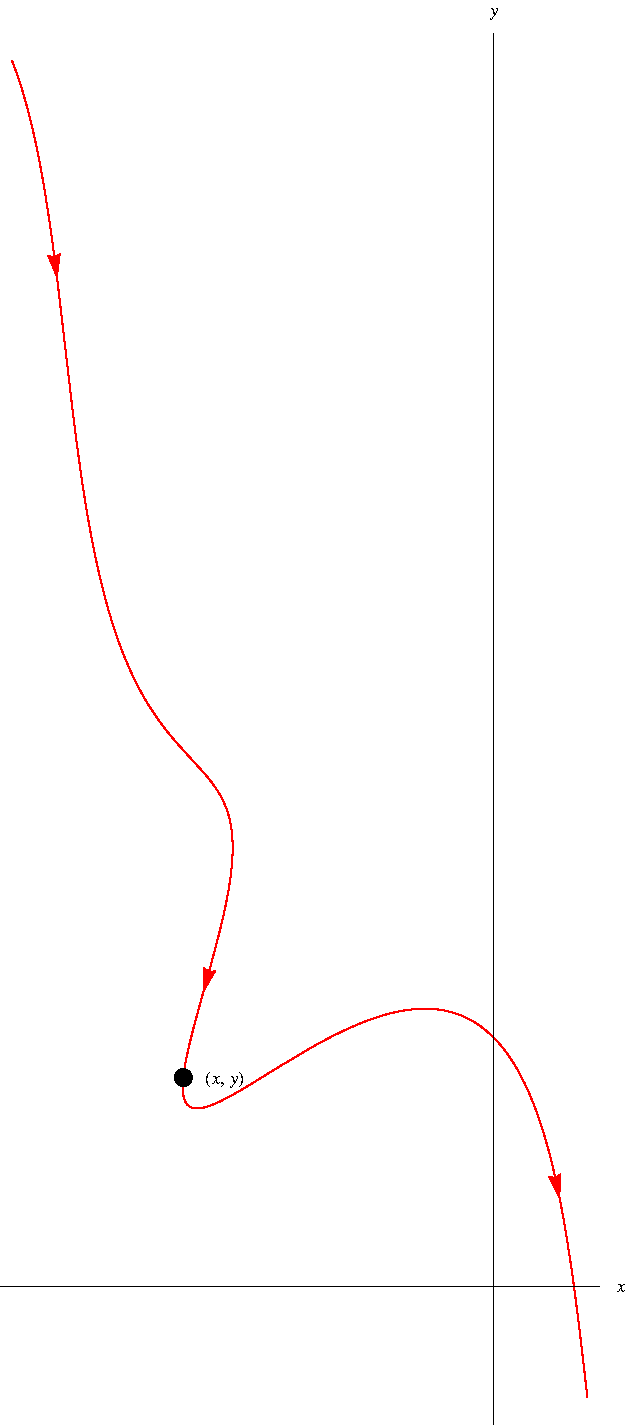
\includegraphics[height=7cm]{parametric-curves/pictures/11-01-parametrice.pdf}%
%}%
%\only<8->{%
%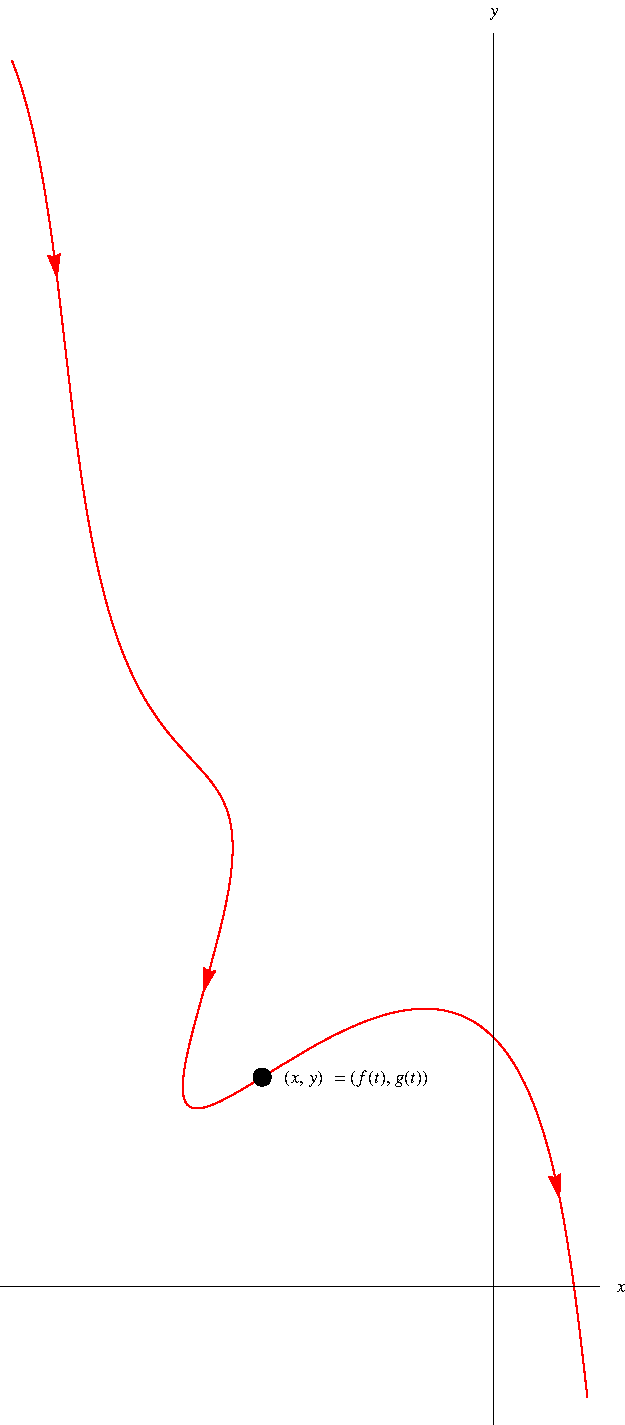
\includegraphics[height=4cm]{parametric-curves/pictures/11-01-parametricf.pdf}%
%}%
\column{.6\textwidth}
\begin{itemize}
\item  Suppose a particle moves along the curve in the picture.
\item<6->  The $x$-coordinate and $y$-coordinate of the particle are some functions of the time $t$.
\item<7->  We can write $x = f(t)$ and $y = g(t)$.
\item<8->  Less formally, we may directly write $(x,y)=(x(t), y(t))$.
\item<9->  We say that the equations $\left| \begin{array}{rcl}x &=& f(t)\\y&=&g(t)\end{array}\right.$ are parametric equations of a parametric curve.
\item<9->  Note that the curve can't be written as $y = f(x)$: it fails the vertical line test.
\end{itemize}
\end{columns}
\end{frame}
% end module parametric-intro


%%begin module parametric-curve-vs-curve-image-terminology
\begin{frame}
\begin{columns}
\column{0.5\textwidth}
\begin{center}
\psset{xunit=1.5cm, yunit=1.5cm}
\begin{pspicture}(-1.000000, -5)(1.500000,5) 
\psframe*[linecolor=white](-1.000000,-5)(1.500000,5) 
\tiny 
\psaxesStandard{-0.200000}{-0.2}{1.2}{1.2}
\psline[linecolor=\psColorGraph](0,0)(1,1)
\rput[l](0.4,0.2){$C_1:
\left| 
\begin{array}{rcl}
x&=&t^2\\
y&=&t^2\\
\end{array} \right., t\in [0,1]
$}
\end{pspicture} 
\end{center}

\column{0.5\textwidth}
\begin{center}
\psset{xunit=1.5cm, yunit=1.5cm}
\begin{pspicture}(-1.000000, -5)(1.500000,5) 
\psframe*[linecolor=white](-1.000000,-5)(1.500000,5) 
\tiny 
\psaxesStandard{-0.200000}{-0.2}{1.2}{1.2}
\psline[linecolor=\psColorGraph ](0,0)(1,1)
\rput[l](0.4,0.2){$C_2:
\left| 
\begin{array}{rcl}
x&=&t\\
y&=&t\\
\end{array} \right., t\in [0,1]$
}
\end{pspicture}
\end{center}
\end{columns}
\begin{question}
$\begin{array}{l|l}
\only<1-3>{\text{ Are the above curves different?}}
\only<4->{\alert<4>{\xcancel{\text{ Are the above curves different?}}}} &\begin{array}{l} \uncover<2->{\alert<2>{\text{Are the above parametric curves} }
\\
\alert<2>{\text{different? Yes.}}}
\\
\uncover<3->{\alert<3>{\text{Are the above curve images}}\\ 
\alert<3>{\text{ different? No.}}}
\end{array}
\end{array}
$
\end{question}
\begin{itemize}
\only<1-4>{
\item<2-> As parametric curves, $C_1$ and $C_2$ are different: $C_1, C_2$ are given by different functions.
\item<3-> As curve images, $C_1,C_2$ coincide.
\item<4-> The original question is incorrectly posed: the word ``curve'' does not have a mathematical definition without the words ``parametric'' or ``image'' attached to it.
}
\item<5-> Nonetheless we sometimes use the word ``curve'' \alert<5>{informally}, without specifying ``parametric curve'' or ``curve image''. 
\item<6-> In this case, whether we mean  ``parametric curve'' or ``curve image'' should be clear from the context. \uncover<7->{\alert<7>{If not, we are using mathematical language incorrectly.}}
\end{itemize}

\vspace{5cm}

\end{frame}



%end module parametric-curve-vs-curve-image-terminology

%%begin module curve-image-definition-intro
\begin{frame}
Consider the two parametric curves:
\begin{columns}
\column{0.5\textwidth}
\[
\gamma_1:
\left|
\begin{array}{rcl}
x&=&t^2\\
y&=&t^2\\
\end{array} \right., t\in [0,1]\quad
\]
\begin{center}
\psset{xunit=2cm, yunit=2cm}
\begin{pspicture}(-0.5, -0.5)(1.4,1.4)
\psframe*[linecolor=white](-0.5, -0.5)(1.400000,1.4)
\tiny
\fcAxesStandard{-0.200000}{-0.2}{1.2}{1.2}
\uncover<8->{
\psline[linecolor=\fcColorGraph](0,0)(1,1)
}
\uncover<2->{
\fcFullDot{0}{0}
}
\uncover<3->{
\fcFullDot{0.04}{0.04}
}
\uncover<4->{
\fcFullDot{0.16}{0.16}
}
\uncover<5->{
\fcFullDot{0.36}{0.36}
}
\uncover<6->{
\fcFullDot{0.64}{0.64}
}
\uncover<7->{
\fcFullDot{1}{1}
}
\end{pspicture}
\end{center}

\column{0.5\textwidth}
\[
\gamma_2:
\left|
\begin{array}{rcl}
x&=&t\\
y&=&t\\
\end{array} \right., t\in [0,1]\quad
\]
\begin{center}
\psset{xunit=2cm, yunit=2cm}
\begin{pspicture}(-0.5000000, -0.5)(1.400000,1.4)
\psframe*[linecolor=white](-0.5000000, -0.5)(1.400000,1.4)
\tiny
\fcAxesStandard{-0.200000}{-0.2}{1.2}{1.2}
\uncover<8->{
\psline[linecolor=\fcColorGraph ](0,0)(1,1)
}
\uncover<2->{
\fcFullDot{0}{0}
}
\uncover<3->{
\fcFullDot{0.2}{0.2}
}
\uncover<4->{
\fcFullDot{0.4}{0.4}
}
\uncover<5->{
\fcFullDot{0.6}{0.6}
}
\uncover<6->{
\fcFullDot{0.8}{0.8}
}
\uncover<7->{
\fcFullDot{1}{1}
}
\end{pspicture}
\end{center}
\end{columns}
\uncover<2->{Plug in} \uncover<2->{\alert<2>{$ t=0 $}}\uncover<3->{, \alert<3>{$t=0.2$}}\uncover<4->{, \alert<4>{$t = 0.4 $}}\uncover<5->{, \alert<5>{$t = 0.6$}}\uncover<6->{, \alert<6>{$t=0.8$}}\uncover<7->{, \alert<7>{$t = 1$}.}
\uncover<9->{
\begin{question}
Are the above curves different?
\end{question}
}
\uncover<10->{
To answer this question we need a definition.
}
\end{frame}
%end module curve-image-definition-intro

%
\begin{frame}
Recall a parametric curve $\gamma$  was defined as the data
\[
\gamma:
\left| 
\begin{array}{rcl}
x_1&=&f_1(t)\\
x_2&=&f_2(t)\\
&\vdots & \\
x_n&=&f_n(t)
\end{array} \right., t\in [a,b]\quad 
\]
\begin{definition}
A \emph{curve image} (or simply a curve) is any set of points that arises by traversing some \alert<2>{continuous} curve. In other words, a curve image is any set that can be written in the form
\[
\left\{(f_1(t),\dots, f_n(t))~|~ t\in [a,b]\right\}\quad ,
\]
for some \alert<2>{continuous} functions $f_1, \dots, f_n$.
\end{definition}
\only<2>{If we don't require that the functions be continuous, every set of points will be a curve and the definition would be pointless.}

\uncover<3->{Informally, a curve image ``remembers'' only the points lying on the curve but forgets the ``speed'' with which each point was visited and ``how many times'' each point was visited.
}
\end{frame}

%%begin module area-under-hyperbola-ex1

\begin{frame}
Recall Euler substitution: $x=\frac12\left(\frac{1}{t}- t \right)$, $\alert<2>{\sqrt{x^2+1}=\frac{1}2\left(\frac 1 t +t\right)}$, $\alert<12,13,14>{ t=\sqrt{x^2+1}-x} $, $\alert<3>{ \diff x=-\frac12 \left(\frac1{t^2} +1\right)\diff t}$.
\begin{example}
$
\begin{array}{rcl}
\displaystyle \int \alert<2>{ \sqrt{x^2+1}} \alert<3>{\diff x} \vphantom{ \frac{1}{8}\left(\frac{1}{ (\sqrt{ x^2 +1} -x)^2} - (\sqrt{x^2+1}- x)^2 \right) } &=&
\displaystyle
\only<1-16>{
\uncover<2->{ \alert<3>{-} \int  \alert<2>{\alert<4>{\frac12} \left(\alert<5,6>{\frac1t} +\alert<7,8>{t}\right)} \alert<3>{\alert<4>{ \frac{1}{2}} \left(\alert<5,7>{ \frac 1 {t^2}} +\alert<6,8>{1} \right)\diff t}} \\
\uncover<4->{ &=&\displaystyle -\alert<4>{ \frac 1 4} \alert<9,10,11>{ \int} \left(\alert<5>{ \alert<9>{ \frac{ 1 }{ t^3}}} + \alert<6,7,10>{2\frac{1}t} + \alert<8,11>{t} \right) \alert<9,10,11>{ \diff t} } \\
\uncover<9->{&=&\displaystyle \alert<15>{-\frac{1}4} \left( \alert<9>{ \alert<15>{ -}\frac{ \alert<12>{ t^{-2}}}{\alert<15>{2}}} +\alert<10>{ \alert<15>{2} \ln\alert<14>{ |t|} }+ \alert<11>{\frac{\alert<13>{ t^2}}{\alert<15>{2}}} \right)+C}\\
\uncover<12->{&=&}
}
\uncover<12->{\displaystyle \only<1-24>{  \alert<16,17,18,24>{ \alert<15>{\frac{1}{8}} \left(\frac{1}{\alert<12>{ (\sqrt{ x^2 +1} -x)^2}} - \alert<13>{\left(\sqrt{x^2+1}- x\right)^2} \right) } }}\only<25->{
\alert<25>{ \frac{1}{2}x\sqrt{x^2+1}}
} {~~~~~~~~~~~~~~~~~~~~~~~~~~~~~~~~~~~~~~~~~~~~~~~~~~~~~~}  \\
\uncover<12->{ && \displaystyle \alert<16,17>{ \only<1-30>{\alert<15>{ -}} \only<31->{\alert<31>{+} } \alert<15>{ \frac12}  \alert<26,30>{\ln \left( \alert<14>{ \sqrt{x^2+1} \only<1-30>{-}\only<31->{\alert<31>{+} } x} \right)} +C}}
\end{array}
$

\noindent \only<17-25>{The answer is good. However, let's simplify.

\noindent
\uncover<18->{
$
\begin{array}{l}
\phantom{=}
\displaystyle \alert<18>{ \frac{1}{(\sqrt{x^2+1}-x)^2}- \left( \sqrt{ x^2+1 }-x\right)^2} \\
\uncover<19->{= \displaystyle \frac{ \alert<19>{(\sqrt{x^2+1} +x )^2} }{ ( \sqrt{x^2 +1} -x )^2  	\alert<19>{(\sqrt{x^2+1}+x)^2} } - \left(\sqrt{x^2+1}-x\right)^2} \\
\uncover<20->{ =\displaystyle \frac{(\sqrt{x^2+1}+x)^2}{ \alert<20>{ \alert<21,22>{((\sqrt{x^2 +1 } )^2 -x^2 )^2 } \uncover<21,22>{\alert<21,22>{=1}} } } - \left( \sqrt{x^2 +1 } -x \right)^2} \\
\displaystyle \uncover<22->{=\left(\sqrt{x^2+1}+x\right)^2-\left( \sqrt{ x^2 + 1 } -x\right)^2} \uncover<23->{ = \alert<24,25>{ 4x\sqrt{x^2+1}}}
\end{array}
$
} %uncover<18->
} %only<17-25>

\only<26->{
The last expression can be transformed to:
\[
\begin{array}{rcl}
\displaystyle
\alert<26>{\ln} \left(\frac{\alert<26,28>{\left(\sqrt{x^2+1}-x\right)} \uncover<27->{ \alert<27,28>{\left( \sqrt{x^2+1}+ x \right)} }}{ \uncover<27->{ \alert<27>{ \sqrt{x^2 +1} +x}}} \right)
&=& \displaystyle \uncover<28->{\alert<29>{ \ln \left( \frac{\alert<28>{ 1} }{ \sqrt{x^2+1}+x}\right)} }\\ \uncover<29->{&=&\alert<29,30,31>{ -\ln \left(\sqrt{x^2+1}+x\right)}}
\end{array}
\]
}
\end{example}

\vspace{8cm}
\end{frame}

\begin{frame}
\begin{example}
Find the area locked b-n the hyperbolas $\alert<2,3>{ y=\pm \sqrt{ x^2+1}}$ and $x=\pm 2\sqrt{ 2}$.
\begin{columns}
\column{.5\textwidth}
\psset{xunit=0.7cm, yunit=0.7cm}
\begin{pspicture}(-3.328427, -3)(3.328427,3)
\psframe*[linecolor=white](-3.328427,-3)(3.328427,3)
\tiny
\uncover<31->{
\pscustom*[linecolor=\fcColorAreaUnderGraph]{
\psplot[linecolor=\fcColorGraph, plotpoints = 1000 ] {-2.828427} {2.828427}{1 x 2 exp add 0.5 exp }
\psline[linecolor=\fcColorGraph](2.828427,-3)(2.828427,3)
\psplot[linecolor=\fcColorGraph, plotpoints=1000] { 2.828427 } {-2.828427}{1 x 2 exp add 0.5 exp -1 mul }
\psline[linecolor=\fcColorGraph](-2.828427,-3)(-2.828427,3)
}
}
\uncover<1-26,28->{
\psaxes[arrows=<->,ticks=none, labels=none](0,0)(-3,-3)(3,3)
}
\psline[linecolor=red!1](3.301,2)(3.302,2)
\psline[linecolor=red!1](-3.301,2)(-3.302,2)

%Function formula: - (x^{2}+1)^{1/2}
\psplot[linecolor=\fcColorGraph, plotpoints=1000]{-2.828427}{2.828427}{1 x 2 exp add 0.5 exp -1 mul }
\uncover<3-4>{\rput[tl](-2.2, -2.4){ \alert<3>{ $y= - \sqrt{ x^2 +1 }$}}}

%Function formula: (x^{2}+1)^{1/2}
\psplot[linecolor=\fcColorGraph, plotpoints=1000]{-2.828427}{ 2.828427 }{1 x 2 exp add 0.5 exp }
\uncover<2-4>{\rput[bl](-2.1, 2.4){\alert<2>{ $y=\sqrt{ x^2 +1} $}}}

\uncover<29->{
\psline[linecolor=\fcColorGraph](-2.828427,3)(-2.828427,-3)
}
\uncover<30->{
\psline[linecolor=\fcColorGraph](2.828427,3)(2.828427,-3)
}
\uncover<25-27>{
\psline{<->}(-2.9,2.9)(2.9,-2.9)
\rput[t](-2.1, 1.7){$\begin{array}{l} \alert<25>{v=0} \\\uncover<1-26>{\alert<25>{y+x=0}} \end{array}$}
}
\uncover<15-27>{
\psline{<->}(-2.9,-2.9)(2.9,2.9)
\rput[b](-2.1, -1.9){$\begin{array}{l} \uncover<1-26>{ \alert<15>{ y-x=0 }}\\\uncover<16->{\alert<16>{u=0}} \end{array}$}
}
\uncover<17-26>{
\fcFullDot{1.4}{1.4}
\rput[l]( 1.6, 1.4){$(\frac{y+x}{2},\frac{y+x}{2})$}
}
\uncover<14-26>{
\fcFullDot{0.6}{2.2}
\rput[lb](0.65, 2.2){$(x,y)$}
}
\uncover<26>{
\psline(0.6,2.2)(-0.8,0.8)
\psline(-0.7, 0.9)(-0.6, 0.8)(-0.7, 0.7)
\rput[rb](-0.3, 1.3){\alert<26>{$v$}}
}
\uncover<18-26>{
\psline(0.6,2.2)(1.4, 1.4)
\psline(1.3, 1.5)(1.2,1.4)(1.3, 1.3)
}
\uncover<23-26>{
\rput[tr](0.95, 1.8){\alert<23>{$u$}}
}
\uncover<14-26>{
\fcFullDot{2.2}{0.6}
\rput[lt]( 2.2, 0.65){$(y,x)$}
}
\end{pspicture}

\vbox to 3.0cm {
\uncover<18->{\alert<18>{
\uncover<22->{\alert<22>{Signed}} distance b-n $(x,y)$ and line $u=0$ equals}}
\only<1-23>{
$\uncover<19->{\uncover<22->{\alert<22>{\pm}} \alert<19>{ \sqrt{ \alert<20>{ \left(x-\frac{(x+y)}{2} \right)^2+ \left( y- \frac{(x+y )}{2} \right)^2}}}}
$
$\uncover<20->{=\uncover<22->{\alert<22>{\pm}} \sqrt{ \alert<20>{ \frac{1}{2}(y-x)^2 }}} \uncover<21->{= \alert<21>{ \uncover<1-21>{\pm} \alert<23>{ \frac{\sqrt{2 }}{ 2 } ( y-x)}}} \uncover<23>{ \alert<23>{=}}$
} %only<1-23>
\uncover<23->{ \alert<23,24>{$u $}.}
\only<24->{\uncover<25->{
Similarly compute that \alert<26>{signed distance b-n $(x,y)$ and the \alert<25>{line $v=0$} equals $v$}.
\uncover<27->{$\Rightarrow$ $y^2-x^2=1$ is the \alert<27>{ hyperbola $v=\frac{1/2}{v}$} in the $(u,v)$-plane.}
}}

\vfil
} %vbox

\column {.5\textwidth}
\only<1-27>{
\uncover<4->{We studied $\alert<27>{v=\frac{1/2}{u}}$ is called a hyperbola:}\uncover<3->{ why do we call $y= \sqrt{ x^2 +1}$ hyperbola?} \uncover<5->{Compute:}
\[
\begin{array}{rcl}
\uncover<5->{\sqrt{x^2+1} &=& y}\\
\uncover<6->{ x^2+1 &=& y^2}\\
\uncover<7->{y^2-x^2&=&1}\\
\uncover<8->{\uncover<9>{\alert<9>{\frac{1}{2}}} \uncover<10->{\alert<10,11>{\frac{\sqrt{2}}{2}}} \alert<11>{(y-x)} \uncover<10->{\alert<10,12>{\frac{\sqrt{2}}{2}}} \alert<12>{(y+x)}&=&\uncover<9->{\alert<9>{\frac{1}{2}}} \uncover<8>{1}}\\
\uncover<11->{\alert<11>{u}\alert<12>{v}&=& \frac{1}{2}}\\
\uncover<13->{\alert<27>{v}&\alert<27>{=}& \alert<27>{\frac{1/2}{u}},}
\end{array}
\]
\uncover<11->{where $\begin{array}{|l}
\alert<11,16,23>{u=\frac{\sqrt{2}}{2} \left(y-x\right)}\\
\alert<12,25>{v=\frac{\sqrt{2}}{2}\left(y+x\right)}
\end{array}$. } \uncover<14->{Consider an arbitrary point $(x,y)$.}
} %only<1-27>
\only<28->{
The area in question is:
$
\begin{array}{l}
\displaystyle\phantom{=} \int \limits^{{{\uncover<28,29>{\alert<29>{ \textbf{?}}}\uncover<30->{\alert<30>{ 2\sqrt{2}}}}}}_{\uncover<28>{\alert<28>{\textbf{?}}}\uncover<29->{ -2\sqrt{2}}} 2\sqrt{x^2+1}\diff x \\
\displaystyle \uncover<32->{= \uncover<33->{\alert<33>{2}} \left[x\sqrt{x^2+1} \vphantom{\ln \left(\sqrt{x^2+1}+x\right) }\right.}\\
\displaystyle \uncover<32->{\left. \ln \left(\sqrt{x^2+1}+x\right)\right]^{2\sqrt{2}}_{\only<33->{\alert<33>{0}} \uncover<1-32>{-2\sqrt{2}}}}\\
\uncover<34->{=2\left(2\sqrt{2} \sqrt{(2\sqrt{2})^2+1}\right.} \\
\uncover<34->{\left.+ \ln \left(\sqrt{(2\sqrt{2})^2+1}+2\sqrt{2} \right) \right)}\\
\uncover<35->{=12\sqrt{2} +2\ln \left(3+2\sqrt{2}\right )}\\
\uncover<36->{\approx 20.496}
\end{array}
$
}
\end{columns}

\end{example}

\end{frame}

%end module area-under-hyperbola-ex1



%% begin module polar-area-justification
\begin{frame}[t]
\begin{columns}
\frametitle{Area swept by a polar curve: justification}
\column{0.5\textwidth}
\psset{xunit=1cm, yunit=1cm, algebraic=false}
\begin{pspicture}(-2.65,-1)(1.4,2.3)%
\tiny%
\psline[linecolor=red!1](1.4, 2.3)(1.39, 2.3)%
\psline[linecolor=red!1](-2.65, -1)(-2.649, -1)%
\rput[t](0,-0.1){$O$}%
\pstVerb{%
10 dict begin
/thePolarR {t 2 div 1 add} def
/thePolarX {t 57.295779513 mul cos thePolarR mul} def
/thePolarY {t 57.295779513 mul sin thePolarR mul} def
/thetaMax 3.5 def
}%
\uncover<1>{%
\pscustom*[linecolor=cyan]{%
\fcDrawPolar[linecolor=red, plotpoints=1000]{0}{thetaMax}{thePolarR}%
\pstVerb{1 dict begin /t thetaMax def}%
\psline(! thePolarX thePolarY )(0,0)(1,0)%
\pstVerb{end}%
}%
\pstVerb{1 dict begin /t thetaMax def}%
\psline[linecolor=red](! thePolarX thePolarY )(0,0)(1,0)%
\pstVerb{end}%
}%
\rput[t](1.2,-0.1){$x$}%
\uncover<2-15>{%
\rput[b](-0.832294, 1.85){$\alertNoH{4}{P_2}$}%
\rput[bl](0.84, 1.3){$\alertNoH{4}{P_1}$}%
\pstVerb{1 dict begin /t 1 def}%
\fcFullDot{thePolarX}{thePolarY}%
\pstVerb{/t 2 def}%
\fcFullDot{thePolarX}{thePolarY}%
\pstVerb{end}%
}%
\uncover<5-15>{%
\pstVerb{1 dict begin /t 1 def}%
\psline[linecolor=cyan](0,0)(! thePolarX thePolarY)%
\pstVerb{/t 2 def}%
\psline[linecolor=cyan](0,0)(! thePolarX thePolarY)%
\pstVerb{end}%
}%
\uncover<7-15>{%
\fcPolarWedge{1}{2}{thePolarR}%
}%
\uncover<8,9,10>{%
\pstVerb{1 dict begin /t 1 def}%
\psline[linecolor=red, linewidth=2pt](0,0)(! thePolarX thePolarY)%
\pstVerb{/t 2 def}%
\psline[linecolor=red, linewidth=2pt](0,0)(! thePolarX thePolarY)%
\pstVerb{end}%
}%
\uncover<5-15>{%
\rput[bl](0.50, 0.6){$r_1$}%
\rput[l](-0.45, 1.1){$r_2$}%
}%
\uncover<6-15>{%
\fcAngle{1}{2}{0.7}{}%
\fcAngle{0}{2}{0.45}{}%
\fcAngle{0}{1}{0.15}{}%
\rput[bl](0.15, 0.05){$\alertNoH{6}{\theta_1}$}%
\rput[b](0, 0.46){$\alertNoH{6}{\theta_2}$}%
\rput[b](0, 0.73){$ \alertNoH{9,10}{\Delta}$}%
}%
\uncover<handout:2|11-15>{%
\fcPolarWedgeSequence{0}{1}{3}{thePolarR}%
}%
\uncover<handout:2|16>{%
\fcPolarWedgeSequence{0}{0.75}{4}{thePolarR}%
}%
\uncover<handout:2|17>{%
\fcPolarWedgeSequence{0}{0.5}{6}{thePolarR}%
}%
\uncover<handout:2|18>{%
\fcPolarWedgeSequence{0}{0.3}{10}{thePolarR}%
}%
\uncover<handout:2|19>{%
\fcPolarWedgeSequence{0}{0.2}{15}{thePolarR}%
}%
\uncover<handout:2|20->{%
\fcPolarWedgeSequence{0}{0.1}{30}{thePolarR}%
}%
\fcDrawPolar[linecolor=red, plotpoints=1000]{0}{3.5}{thePolarR}%
\psline[arrows=->](0,0)(1.2, 0)%
\pstVerb{end}%
\end{pspicture}

\column{0.5\textwidth}
\uncover<2->{Split $[a,b]$ into $N$ equal segments via points $a=\theta_0 \leq \theta_1 \leq \dots \leq \theta_{N-1} \leq \theta_N=b$.} \uncover<3->{The length of each segment is $\Delta=\frac{b-a}{N}$.} \uncover<4->{Let $r_i=f(\theta_i)$. Then each $\theta_i$ gives a \alertNoH{4}{point $P_i$} with polar coordinates $(\alertNoH{5}{r_i},\alertNoH{6}{\theta_i})$.}
\end{columns}

\only<handout:1|1-12>{ \uncover<7->{The area swept by the curve is approximated by sum of areas of triangles given by connecting the origin with two consecutive vertices. Consider one such triangle, say, $OP_1P_2$.} \uncover<8->{By Euclidean geometry, the area of $\triangle OP_1P_2 $ is $\alertNoH{8,9}{\frac{|OP_1| |OP_2|  \fcAnswer{9}{ \sin \Delta}}{2}} \uncover<10->{=\frac{ r_1 r_2 \sin \Delta}{2}= \frac{ f(\theta_1) f(\theta_2) \sin \Delta}{2}} $.}
}

\uncover<handout:2| 11->{\alertNoH{12,13}{ Therefore the area swept by the curve \only<handout:0|1-14>{is approximated by} \only<handout:2|15->{\alertNoH{15}{equals \alertNoH{16-}{the limit} of}} the sum:}
\[\begin{array}{rcl}
\uncover<15->{ A&=&}\alertNoH{12,13}{\uncover<15->{\lim\limits_{\Delta\to 0}} \sum\limits_{i=0}^{N-1} \frac{f(\theta_i)f(\theta_{i+1}) \alertNoH{14}{ \sin \Delta} }{2}} \uncover<14->{= \uncover<15->{ \lim \limits_{\Delta\to 0}} \alertNoH{14}{ \frac{ \sin\Delta}{ \Delta}} \sum\limits_{i=0}^{N-1} \frac{ f( \theta_i) f(\theta_{i} + \Delta)\alertNoH{14}{\Delta}}{2}}\\
\uncover<21->{\uncover<24>{\alertNoH{24}{\text{{\tiny(can be proved)}}}}  &=&   \alertNoH{22,23}{ \lim \limits_{\Delta\to 0}\frac{ \sin\Delta}{ \Delta  }}  \lim \limits_{\alertNoH{24}{\Delta\to 0} } \sum\limits_{i=0}^{N-1} \frac{ f( \theta_i) f( \alertNoH{24}{ \theta_{i} + \Delta} )\Delta}{2} \uncover<22->{=  \fcAnswer{23}{1}\cdot \lim \limits_{\Delta\to 0} \sum\limits_{i=0}^{N-1} \frac{\alertNoH{25}{ f( \theta_i) f(\alertNoH{24}{ \theta_{i}} )} \Delta}{2}}} \\
\uncover<25->{\uncover<27->{{\tiny\text{\alertNoH{27}{(Riemann sum)}}}} &=& \lim \limits_{\Delta\to 0} \sum \limits_{i=0}^{N-1} \frac{ \alertNoH{25}{ f^2( \theta_i)}  \Delta }{2}}\uncover<26->{=  \fcAnswer{27}{  \int\limits_{a}^b \frac{ f^2(\theta)}{2}\diff \theta} }
\end{array}
\]
}
\end{frame}
%end module polar-area-justification


%\begin{frame}
%\begin{pspicture*}(-3,-1)(5.2,2.3)%
%\polarWedge{1}{2}{t 2 div 1 add}
%\end{pspicture*}
%\end{frame}
%% begin module derivative-sine-graph
\begin{frame}
\frametitle{Derivatives of Trigonometric Functions}
\psset{xunit=0.8cm, yunit=0.8cm}
\begin{pspicture}(-7.1, -1.5)(7.1,1.5)
\tiny
\psframe*[linecolor=white](-7.1,-1.3)(7.1,1.3)
\fcAxesStandard{-7}{-1.5}{7}{1.5}
%Function formula: sin{}(x)
\psplot[linecolor=red, plotpoints=1000]{-7}{7}{x 57.29578 mul sin }
\fcLabelYOne
\rput(4.2,1){$y=f(x)=\sin{}(x)$}
\fcXTickWithLabel{1.570796327}{$\frac{\pi}{2}$}
\fcXTickWithLabel{3.141592654}{$\pi$}
\fcXTickWithLabel{4.71238898}{$\frac{3\pi}{2}$}
\fcXTickWithLabel{6.283185307}{$\pi$}
\fcXTickWithLabel{-1.570796327}{$-\frac{\pi}{2}$}
\fcXTickWithLabel{-3.141592654}{$-\pi$}
\fcXTickWithLabel{-4.71238898}{$-\frac{3\pi}{2}$}
\fcXTickWithLabel{-6.283185307}{$-\pi$}

\uncover<handout:0|2->{
\fcFullDot{-4.71238898}{1}
\psline[linewidth=1pt, linecolor=blue](-5.4238898,1)(-4.01238898,1)
}
\uncover<handout:0|4->{
\fcFullDot{-3.141592654}{0}
\psline[linewidth=1pt, linecolor=blue](-3.6365674,0.494974747)(-2.646617907,-0.494974747)
}
\uncover<handout:0|6->{
\fcFullDot{-1.570796327}{-1}
\psline[linewidth=1pt, linecolor=blue](-2.270796327,-1)(-0.870796327,-1)
}
\uncover<handout:0|8->{
\fcFullDot{0}{0}
\psline[linewidth=1pt, linecolor=blue](-0.494974747,-0.494974747)(0.494974747,0.494974747)
}
\uncover<handout:0|10->{
\fcFullDot{1.570796327}{1}
\psline[linewidth=1pt, linecolor=blue](2.270796327,1)(0.870796327,1)
}
\uncover<handout:0|12->{
\fcFullDot{3.141592654}{0}
\psline[linewidth=1pt, linecolor=blue](3.6365674,-0.494974747)(2.646617907,0.494974747)
}
\uncover<handout:0|14->{
\fcFullDot{4.71238898}{-1}
\psline[linewidth=1pt, linecolor=blue](5.4238898,-1)(4.01238898,-1)
}
\end{pspicture}

\psset{xunit=0.8cm, yunit=0.8cm}
\begin{pspicture}(-7.1, -1.5)(7.1,1.5)
\tiny
\psframe*[linecolor=white](-7.1,-1.3)(7.1,1.3)
\fcAxesStandard{-7}{-1.5}{7}{1.5}
\fcLabelYOne
\rput(3.141592654,1){$y=f'(x)$}

%\fcXTickWithLabel{1.570796327}{$\frac{\pi}{2}$}
%\fcXTickWithLabel{3.141592654}{$\pi$}
%\fcXTickWithLabel{4.71238898}{$\frac{3\pi}{2}$}
%\fcXTickWithLabel{6.283185307}{$\pi$}
%\fcXTickWithLabel{-1.570796327}{$-\frac{\pi}{2}$}
%\fcXTickWithLabel{-3.141592654}{$-\pi$}
%\fcXTickWithLabel{-4.71238898}{$-\frac{3\pi}{2}$}
%\fcXTickWithLabel{-6.283185307}{$-\pi$}

\uncover<handout:0|3->{
\fcFullDotBlue{-4.71238898}{0}
}
\uncover<handout:0|5->{
\fcFullDotBlue{-3.141592654}{-1}
}
\uncover<handout:0|7->{
\fcFullDotBlue{-1.570796327}{0}
}
\uncover<handout:0|9->{
\fcFullDotBlue{0}{1}
}
\uncover<handout:0|11->{
\fcFullDotBlue{1.570796327}{0}
}
\uncover<handout:0|13->{
\fcFullDotBlue{3.141592654}{-1}
}
\uncover<handout:0|15->{
\fcFullDotBlue{4.71238898}{0}
}
\uncover<handout:0|17->{
%Function formula: cos{}(x)
\psplot[linecolor=blue, plotpoints=1000]{-7}{7}{x 57.29578 mul cos }
}
%placeholders
\psdot[linecolor=white](-6.95, 1.35)
\psdot[linecolor=white]( 6.95,-1.35)
\end{pspicture}

What is the derivative of $f(x) = \sin x$?  \uncover<16,17->{It looks like $\cos x$.}
\end{frame}
% end module derivative-sine-graph


%% begin module direction-fields-intro
\begin{frame}
\frametitle{(10.2) Direction Fields and Euler's Method} 
\begin{itemize}
\item  Often we don't know how to find explicit solutions to a differential equation.
\item  Nevertheless, we can learn a lot about the solutions using:
\begin{itemize}
\item  A graphical approach (direction fields)
\item  A numerical approach (Euler's method)
\end{itemize}
\item<2->  Today we will discuss direction fields, but not Euler's method.
\end{itemize}
\end{frame}
% end module direction-fields-intro

%% begin module direction-fields-procedure
\begin{frame}
\frametitle{Direction Fields}
\begin{itemize}
\item  How do we sketch the graph of the solution to $y' = x + y$ that satisfies the initial condition $y(0) = 1$?
\item<2->  Make a table of values of $y'$.
\end{itemize}
\begin{columns}[c]

\column{.25\textwidth}
\uncover<2->{%
\[%
\begin{array}{|c|r|}
\hline
\textrm{Point} & y' \\
\hline
\alert<handout:0| 3-4>{(1,0)}&%
\alert<handout:0| 3-4>{\uncover<4->{1}}\\%
\alert<handout:0| 5-6>{(-1,0)}&%
\alert<handout:0| 5-6>{\uncover<6->{-1}}\\%
\alert<handout:0| 7-8>{(0,1)}&%
\alert<handout:0| 7-8>{\uncover<8->{1}}\\%
\alert<handout:0| 9-10>{(0,-1)}&%
\alert<handout:0| 9-10>{\uncover<10->{-1}}\\%
\alert<handout:0| 11-12>{(0,0)}&%
\alert<handout:0| 11-12>{\uncover<12->{0}}\\%
\alert<handout:0| 13-14>{(1,1)}&%
\alert<handout:0| 13-14>{\uncover<14->{2}}\\%
\alert<handout:0| 15-16>{(1,-1)}&%
\alert<handout:0| 15-16>{\uncover<16->{0}}\\%
\alert<handout:0| 17-18>{(-1,1)}&%
\alert<handout:0| 17-18>{\uncover<18->{0}}\\%
\alert<handout:0| 19-20>{(-1,-1)}&%
\alert<handout:0| 19-20>{\uncover<20->{-2}}\\%
\hline
\end{array}
\]%
}%


\column{.45\textwidth}
\psset{xunit=0.3cm, yunit=0.3cm}
\begin{pspicture}(-2.7,-2.7)(2.7,2.7)
\tiny
\psaxesStandard{-2.65}{-2.65}{2.65}{2.65}%
%WARNING THE INCREDIBLY BUGGY LATEX MESSES UP WHITE SPACE. DO NOT USE SPACES
\psXTickWithLabel{1}{$1$}
\psXTickWithLabel{2}{$2$}
\uncover<4->{%
\directionFieldOneTangent{x y add}{1}{0}{0.1}{0.02}{linecolor=blue}%
}%
\uncover<6->{%
\directionFieldOneTangent{x y add}{-1}{0}{0.1}{0.02}{linecolor=blue}%
}%
\uncover<8->{%
\directionFieldOneTangent{x y add}{0}{1}{0.1}{0.02}{linecolor=blue}%
}%
\uncover<10->{%
\directionFieldOneTangent{x y add}{0}{-1}{0.1}{0.02}{linecolor=blue}%
}%
\uncover<12->{%
\directionFieldOneTangent{x y add}{0}{0}{0.1}{0.02}{linecolor=blue}%
}%
\uncover<14->{%
\directionFieldOneTangent{x y add}{1}{1}{0.1}{0.02}{linecolor=blue}%
}%
\uncover<16->{%
\directionFieldOneTangent{x y add}{1}{-1}{0.1}{0.02}{linecolor=blue}%
}%
\uncover<18->{%
\directionFieldOneTangent{x y add}{-1}{1}{0.1}{0.02}{linecolor=blue}%
}%
\uncover<20->{%
\directionFieldOneTangent{x y add}{-1}{-1}{0.1}{0.02}{linecolor=blue}%
}%
\uncover<23>{%
\psline(-2.5,2.5)(2.5,-2.5)%
}%
\uncover<24>{%
\directionFieldOneTangent{x y add}{-2.5}{2.5}{0.1}{0.02}{linecolor=red}%
\directionFieldOneTangent{x y add}{-2}{2}{0.1}{0.02}{linecolor=red}%
\directionFieldOneTangent{x y add}{-1.5}{1.5}{0.1}{0.02}{linecolor=red}%
\directionFieldOneTangent{x y add}{-1}{1}{0.1}{0.02}{linecolor=red}%
\directionFieldOneTangent{x y add}{-0.5}{0.5}{0.1}{0.02}{linecolor=red}%
\directionFieldOneTangent{x y add}{0}{0}{0.1}{0.02}{linecolor=red}%
\directionFieldOneTangent{x y add}{0.5}{-0.5}{0.1}{0.02}{linecolor=red}%
\directionFieldOneTangent{x y add}{1}{-1}{0.1}{0.02}{linecolor=red}%
\directionFieldOneTangent{x y add}{1.5}{-1.5}{0.1}{0.02}{linecolor=red}%
\directionFieldOneTangent{x y add}{2}{-2}{0.1}{0.02}{linecolor=red}%
\directionFieldOneTangent{x y add}{2.5}{-2.5}{0.1}{0.02}{linecolor=red}%
}%
\uncover<25->{%
\directionFieldOneTangent{x y add}{-2.5}{2.5}{0.1}{0.02}{linecolor=blue}%
\directionFieldOneTangent{x y add}{-2}{2}{0.1}{0.02}{linecolor=blue}%
\directionFieldOneTangent{x y add}{-1.5}{1.5}{0.1}{0.02}{linecolor=blue}%
\directionFieldOneTangent{x y add}{-1}{1}{0.1}{0.02}{linecolor=blue}%
\directionFieldOneTangent{x y add}{-0.5}{0.5}{0.1}{0.02}{linecolor=blue}%
\directionFieldOneTangent{x y add}{0}{0}{0.1}{0.02}{linecolor=blue}%
\directionFieldOneTangent{x y add}{0.5}{-0.5}{0.1}{0.02}{linecolor=blue}%
\directionFieldOneTangent{x y add}{1}{-1}{0.1}{0.02}{linecolor=blue}%
\directionFieldOneTangent{x y add}{1.5}{-1.5}{0.1}{0.02}{linecolor=blue}%
\directionFieldOneTangent{x y add}{2}{-2}{0.1}{0.02}{linecolor=blue}%
\directionFieldOneTangent{x y add}{2.5}{-2.5}{0.1}{0.02}{linecolor=blue}%
}%
\uncover<25>{%
\psline(-2,2.5)(2.5,-2)%
}%
\uncover<26>{%
\directionFieldOneTangent{x y add}{-2}{2.5}{0.1}{0.02}{linecolor=red}%
\directionFieldOneTangent{x y add}{-1.5}{2}{0.1}{0.02}{linecolor=red}%
\directionFieldOneTangent{x y add}{-1}{1.5}{0.1}{0.02}{linecolor=red}%
\directionFieldOneTangent{x y add}{-0.5}{1}{0.1}{0.02}{linecolor=red}%
\directionFieldOneTangent{x y add}{0}{0.5}{0.1}{0.02}{linecolor=red}%
\directionFieldOneTangent{x y add}{0.5}{0}{0.1}{0.02}{linecolor=red}%
\directionFieldOneTangent{x y add}{1}{-0.5}{0.1}{0.02}{linecolor=red}%
\directionFieldOneTangent{x y add}{1.5}{-1}{0.1}{0.02}{linecolor=red}%
\directionFieldOneTangent{x y add}{2}{-1.5}{0.1}{0.02}{linecolor=red}%
\directionFieldOneTangent{x y add}{2.5}{-2}{0.1}{0.02}{linecolor=red}%
}%
\uncover<27>{%
\directionFieldOneTangent{x y add}{-2}{2.5}{0.1}{0.02}{linecolor=blue}%
\directionFieldOneTangent{x y add}{-1.5}{2}{0.1}{0.02}{linecolor=blue}%
\directionFieldOneTangent{x y add}{-1}{1.5}{0.1}{0.02}{linecolor=blue}%
\directionFieldOneTangent{x y add}{-0.5}{1}{0.1}{0.02}{linecolor=blue}%
\directionFieldOneTangent{x y add}{0}{0.5}{0.1}{0.02}{linecolor=blue}%
\directionFieldOneTangent{x y add}{0.5}{0}{0.1}{0.02}{linecolor=blue}%
\directionFieldOneTangent{x y add}{1}{-0.5}{0.1}{0.02}{linecolor=blue}%
\directionFieldOneTangent{x y add}{1.5}{-1}{0.1}{0.02}{linecolor=blue}%
\directionFieldOneTangent{x y add}{2}{-1.5}{0.1}{0.02}{linecolor=blue}%
\directionFieldOneTangent{x y add}{2.5}{-2}{0.1}{0.02}{linecolor=blue}%
}%
\uncover<27>{%
\psline(-1.5,2.5)(2.5,-1.5)%
}%
\uncover<28>{%
\directionFieldOneTangent{x y add}{-1.5}{2.5}{0.1}{0.02}{linecolor=red}%
\directionFieldOneTangent{x y add}{-1}{2}{0.1}{0.02}{linecolor=red}%
\directionFieldOneTangent{x y add}{-0.5}{1.5}{0.1}{0.02}{linecolor=red}%
\directionFieldOneTangent{x y add}{-0.5}{1}{0.1}{0.02}{linecolor=red}%
\directionFieldOneTangent{x y add}{0}{0.5}{0.1}{0.02}{linecolor=red}%
\directionFieldOneTangent{x y add}{0.5}{0}{0.1}{0.02}{linecolor=red}%
\directionFieldOneTangent{x y add}{1}{-0.5}{0.1}{0.02}{linecolor=red}%
\directionFieldOneTangent{x y add}{1.5}{-1}{0.1}{0.02}{linecolor=red}%
\directionFieldOneTangent{x y add}{2}{-1.5}{0.1}{0.02}{linecolor=red}%
\directionFieldOneTangent{x y add}{2.5}{-2}{0.1}{0.02}{linecolor=red}%
}%
\end{pspicture}

\ \only<handout:0| -3>{%
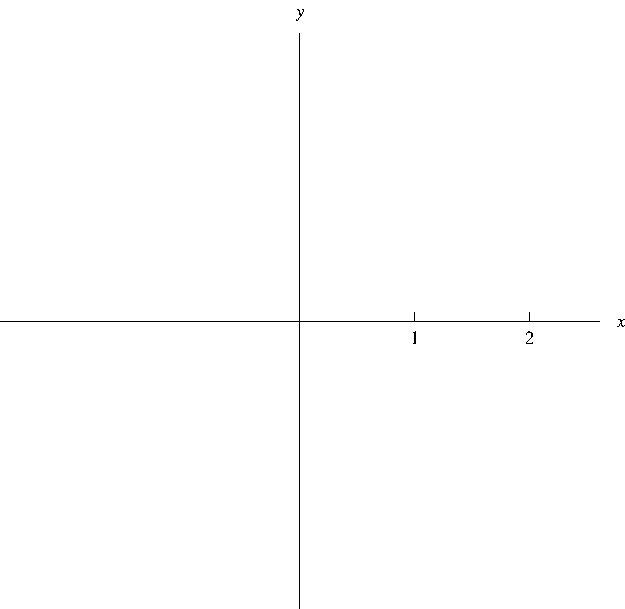
\includegraphics[height=5cm]{diff-eq-direction-fields/pictures/10-02-dirfielda.pdf}%
}%
\only<handout:0| 4>{%
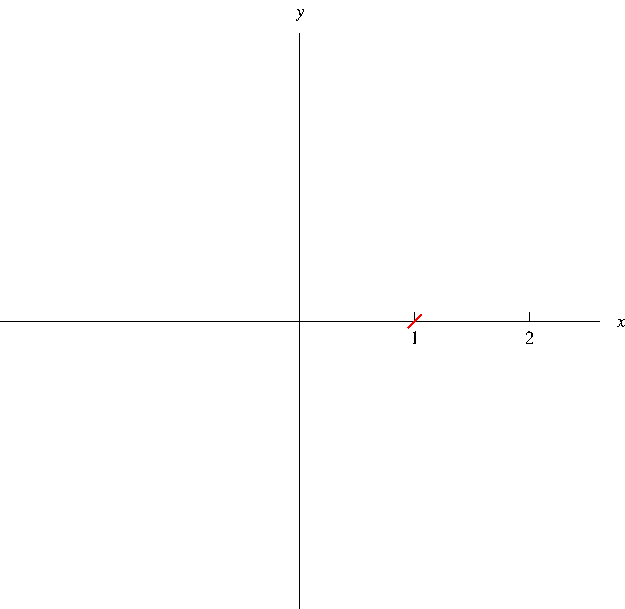
\includegraphics[height=5cm]{diff-eq-direction-fields/pictures/10-02-dirfieldb.pdf}%
}%
\only<handout:0| 5>{%
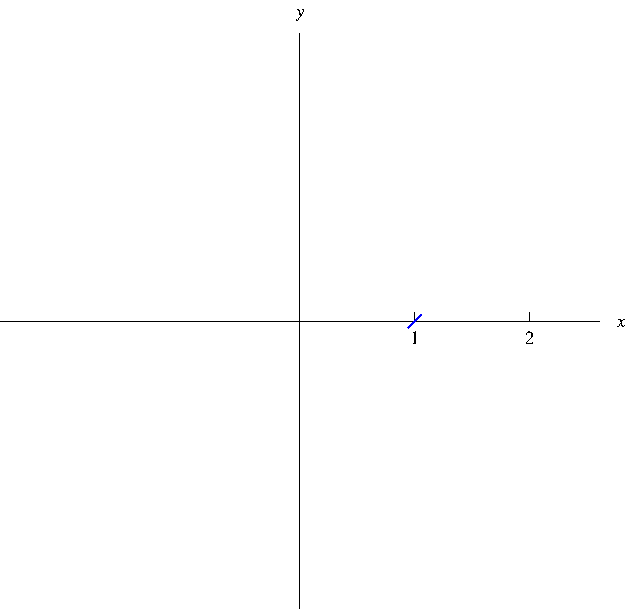
\includegraphics[height=5cm]{diff-eq-direction-fields/pictures/10-02-dirfieldc.pdf}%
}%
\only<handout:0| 6>{%
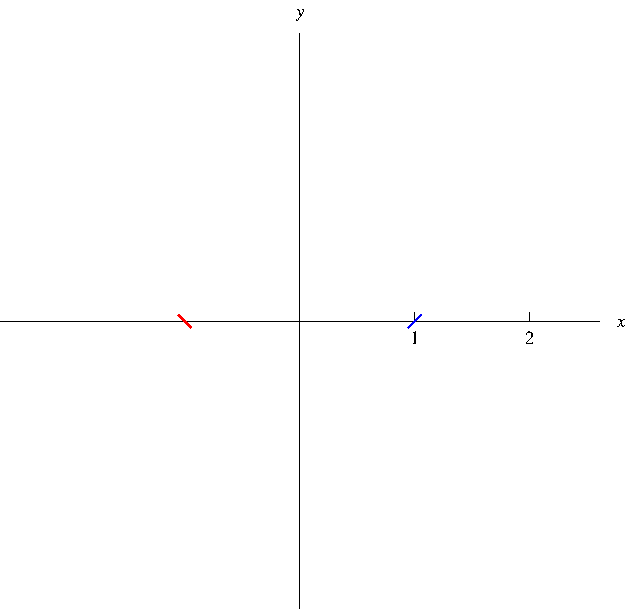
\includegraphics[height=5cm]{diff-eq-direction-fields/pictures/10-02-dirfieldd.pdf}%
}%
\only<handout:0| 7>{%
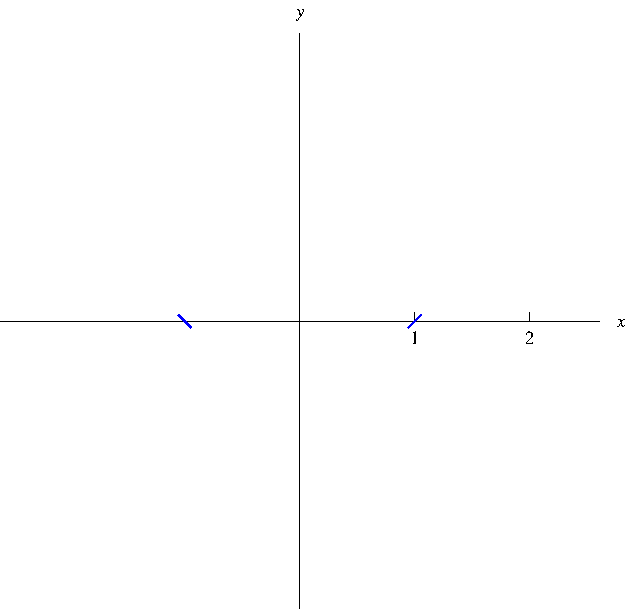
\includegraphics[height=5cm]{diff-eq-direction-fields/pictures/10-02-dirfielde.pdf}%
}%
\only<handout:0| 8>{%
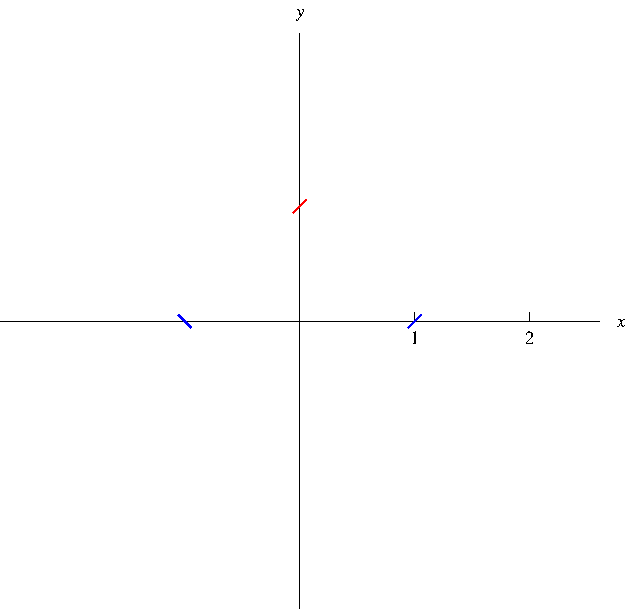
\includegraphics[height=5cm]{diff-eq-direction-fields/pictures/10-02-dirfieldf.pdf}%
}%
\only<handout:0| 9>{%
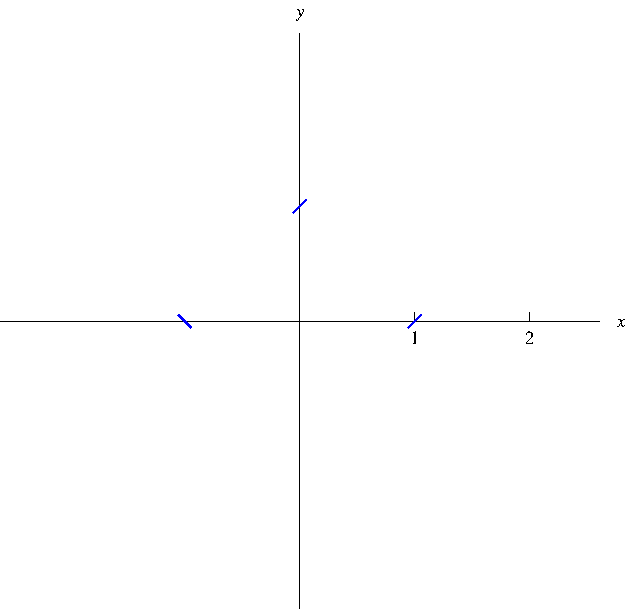
\includegraphics[height=5cm]{diff-eq-direction-fields/pictures/10-02-dirfieldg.pdf}%
}%
\only<handout:0| 10>{%
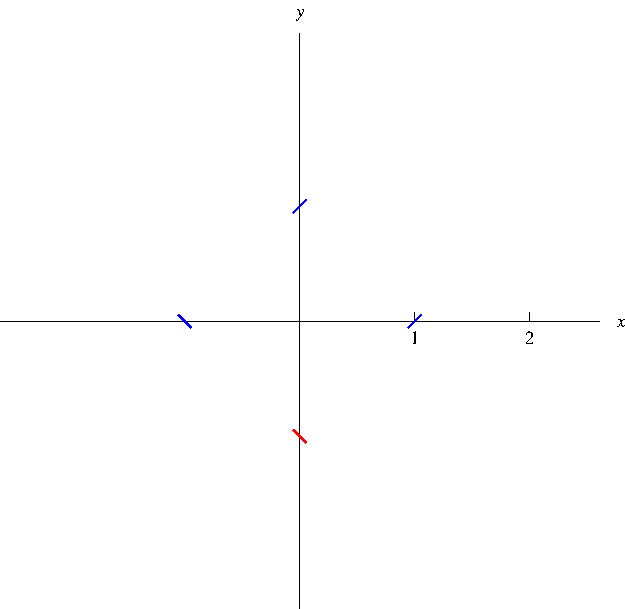
\includegraphics[height=5cm]{diff-eq-direction-fields/pictures/10-02-dirfieldh.pdf}%
}%
\only<handout:0| 11>{%
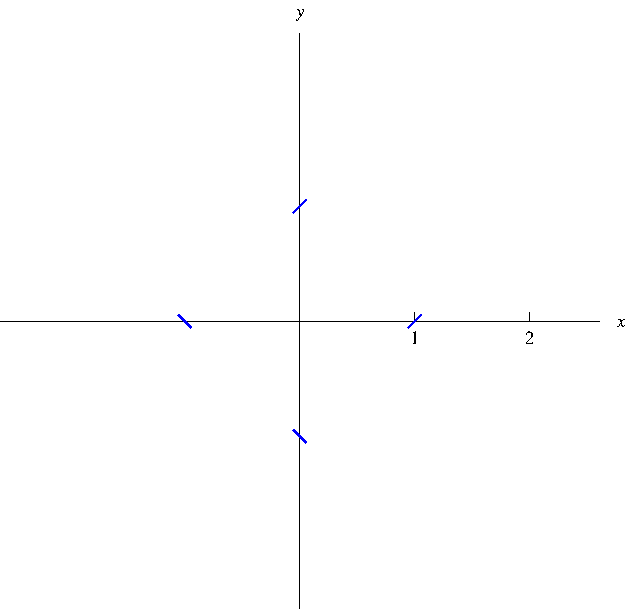
\includegraphics[height=5cm]{diff-eq-direction-fields/pictures/10-02-dirfieldi.pdf}%
}%
\only<handout:0| 12>{%
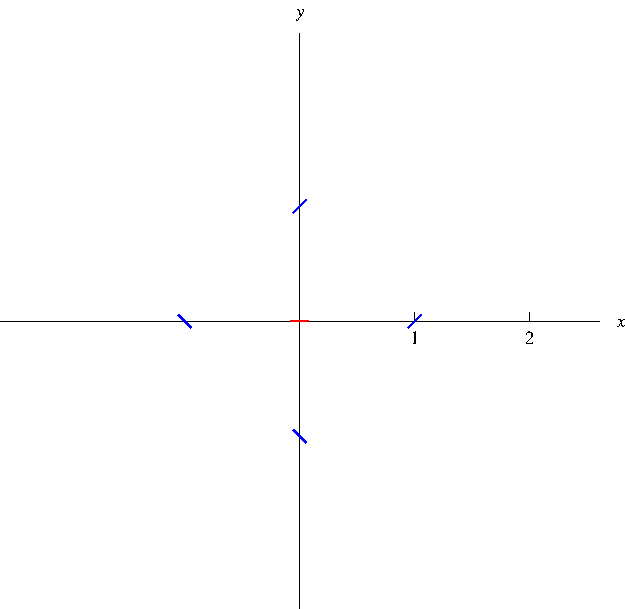
\includegraphics[height=5cm]{diff-eq-direction-fields/pictures/10-02-dirfieldj.pdf}%
}%
\only<handout:0| 13>{%
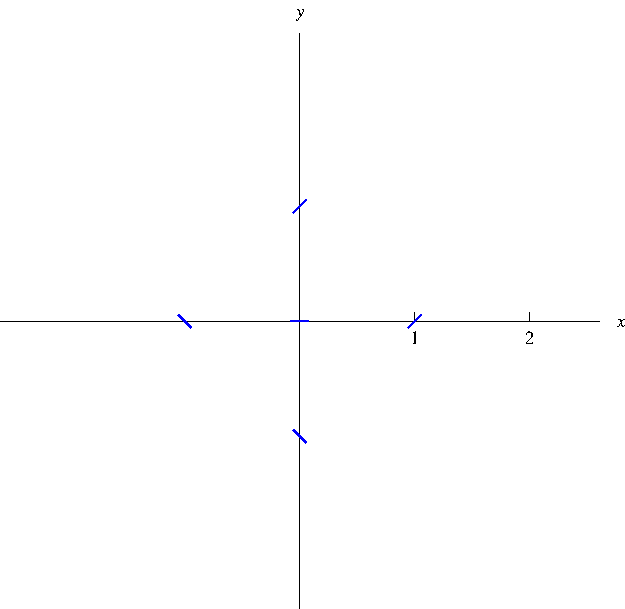
\includegraphics[height=5cm]{diff-eq-direction-fields/pictures/10-02-dirfieldk.pdf}%
}%
\only<handout:0| 14>{%
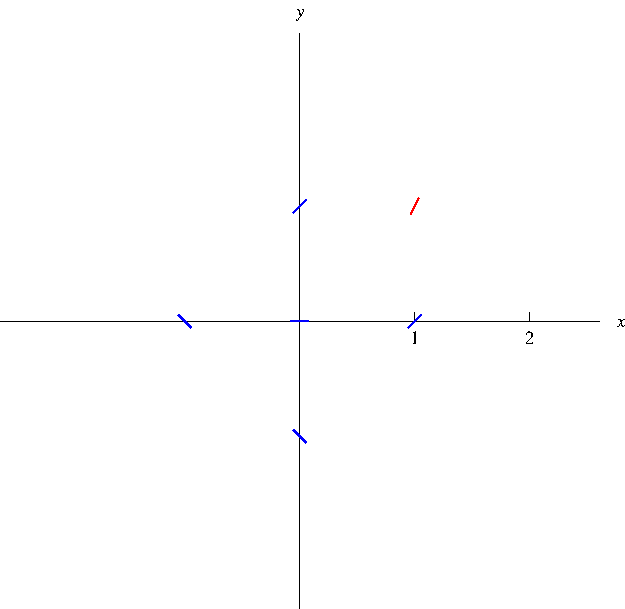
\includegraphics[height=5cm]{diff-eq-direction-fields/pictures/10-02-dirfieldl.pdf}%
}%
\only<handout:0| 15>{%
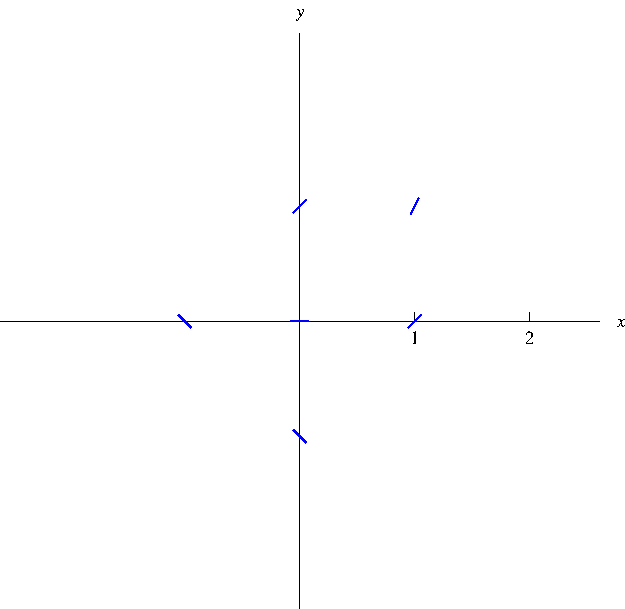
\includegraphics[height=5cm]{diff-eq-direction-fields/pictures/10-02-dirfieldm.pdf}%
}%
\only<handout:0| 16>{%
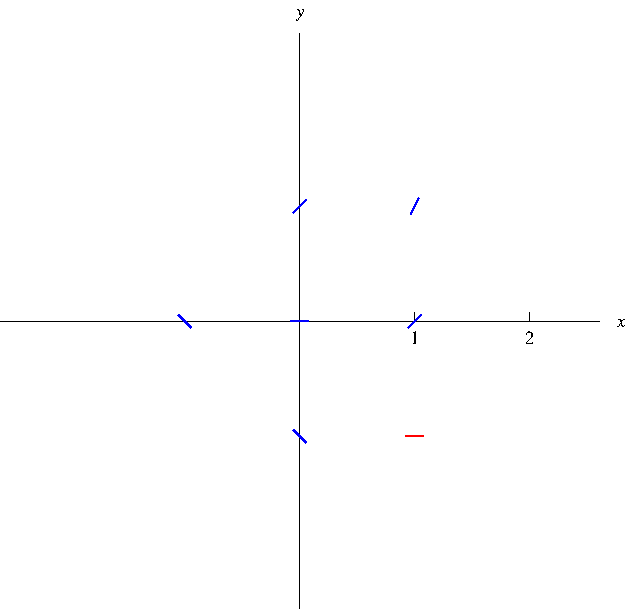
\includegraphics[height=5cm]{diff-eq-direction-fields/pictures/10-02-dirfieldn.pdf}%
}%
\only<handout:0| 17>{%
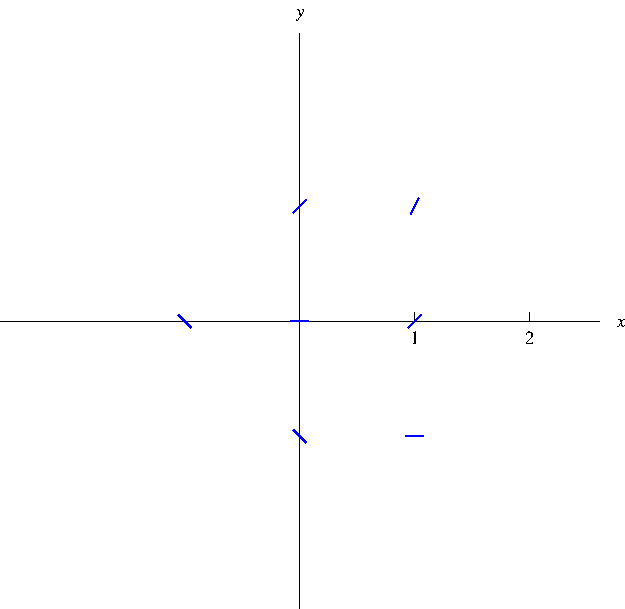
\includegraphics[height=5cm]{diff-eq-direction-fields/pictures/10-02-dirfieldo.pdf}%
}%
\only<handout:0| 18>{%
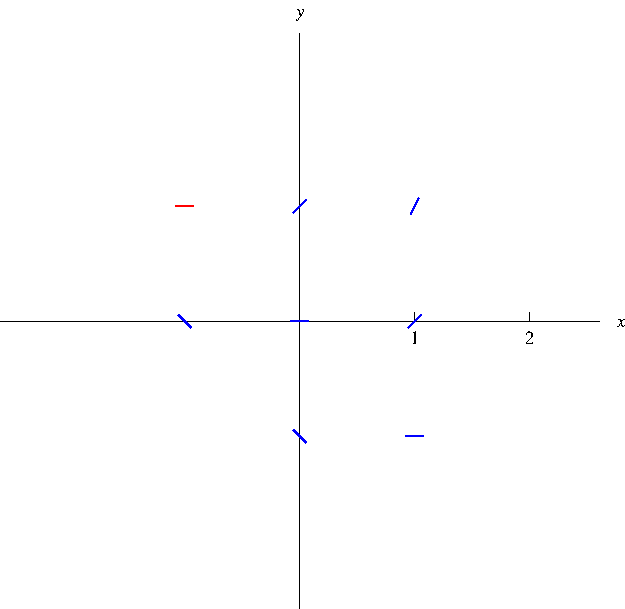
\includegraphics[height=5cm]{diff-eq-direction-fields/pictures/10-02-dirfieldp.pdf}%
}%
\only<handout:0| 19>{%
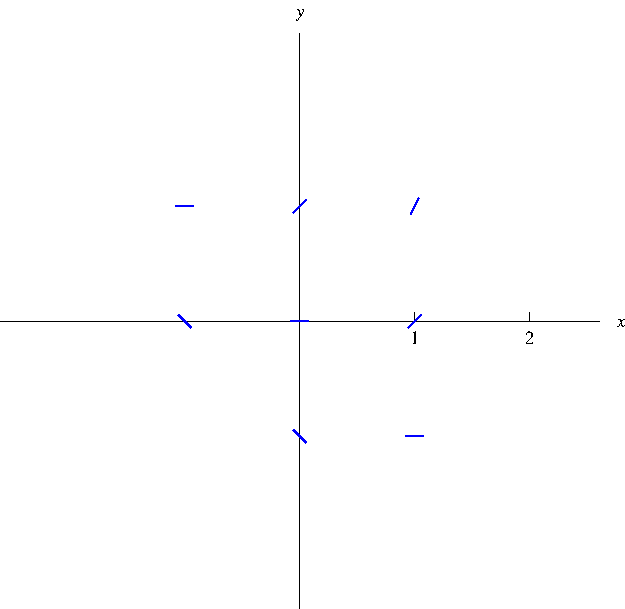
\includegraphics[height=5cm]{diff-eq-direction-fields/pictures/10-02-dirfieldq.pdf}%
}%
\only<handout:0| 20>{%
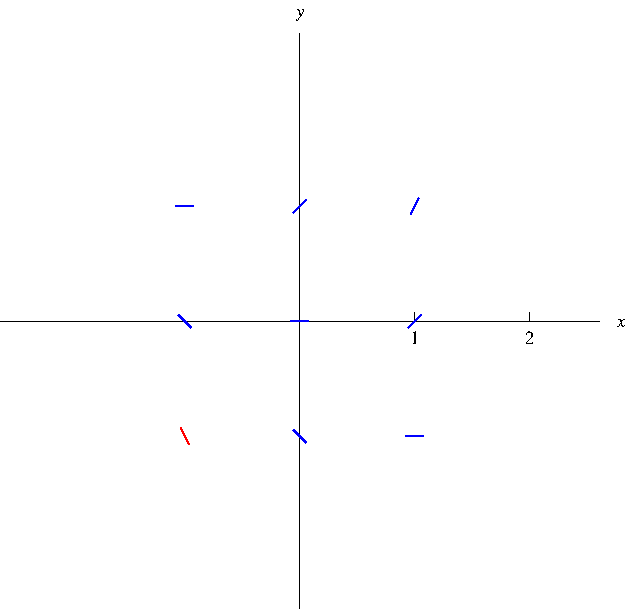
\includegraphics[height=5cm]{diff-eq-direction-fields/pictures/10-02-dirfieldr.pdf}%
}%
\only<handout:0| 21-22>{%
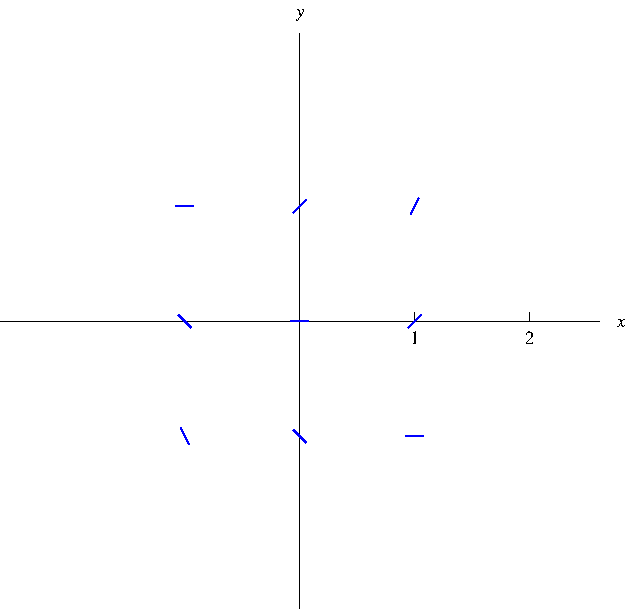
\includegraphics[height=5cm]{diff-eq-direction-fields/pictures/10-02-dirfields.pdf}%
}%
\only<handout:0| 23>{%
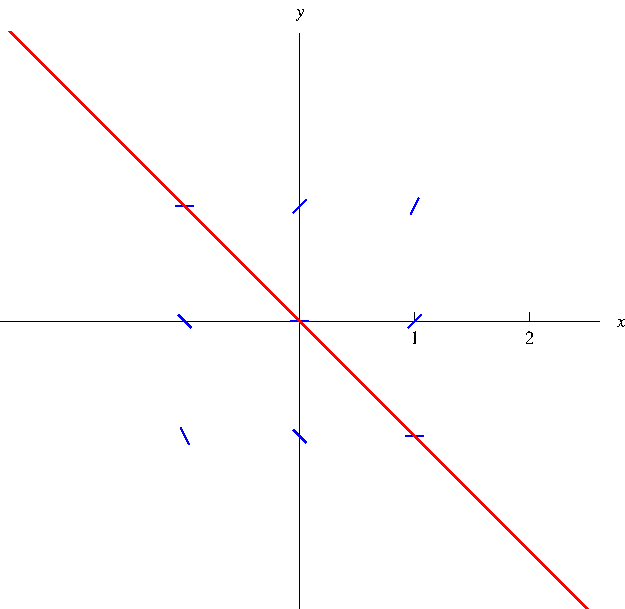
\includegraphics[height=5cm]{diff-eq-direction-fields/pictures/10-02-dirfieldt.pdf}%
}%
\only<handout:0| 24>{%
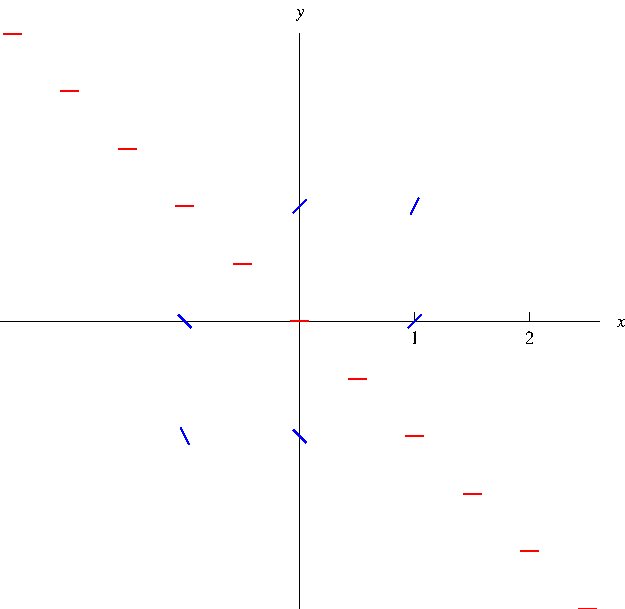
\includegraphics[height=5cm]{diff-eq-direction-fields/pictures/10-02-dirfieldu.pdf}%
}%
\only<handout:0| 25>{%
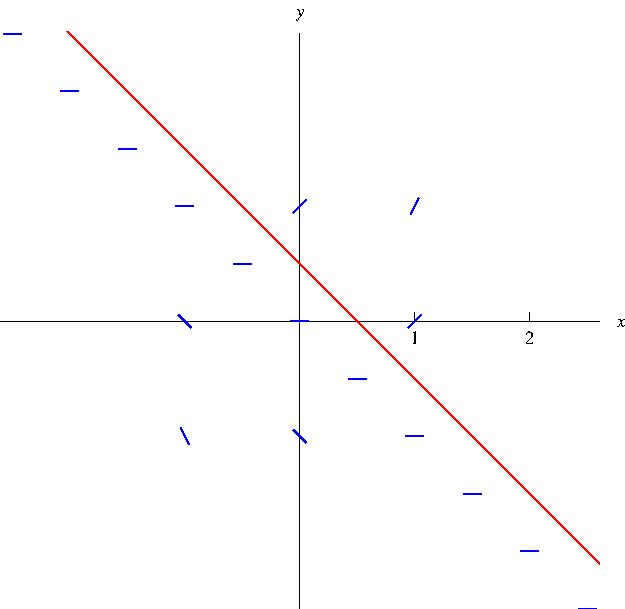
\includegraphics[height=5cm]{diff-eq-direction-fields/pictures/10-02-dirfieldv.pdf}%
}%
\only<handout:0| 26>{%
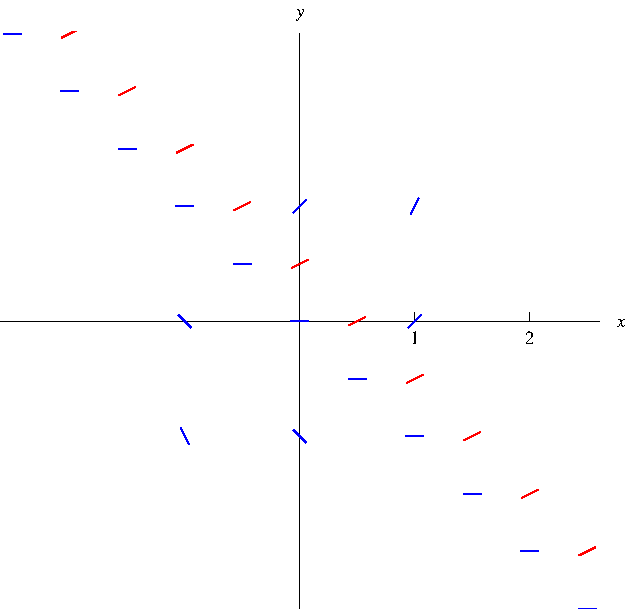
\includegraphics[height=5cm]{diff-eq-direction-fields/pictures/10-02-dirfieldw.pdf}%
}%
\only<handout:0| 27>{%
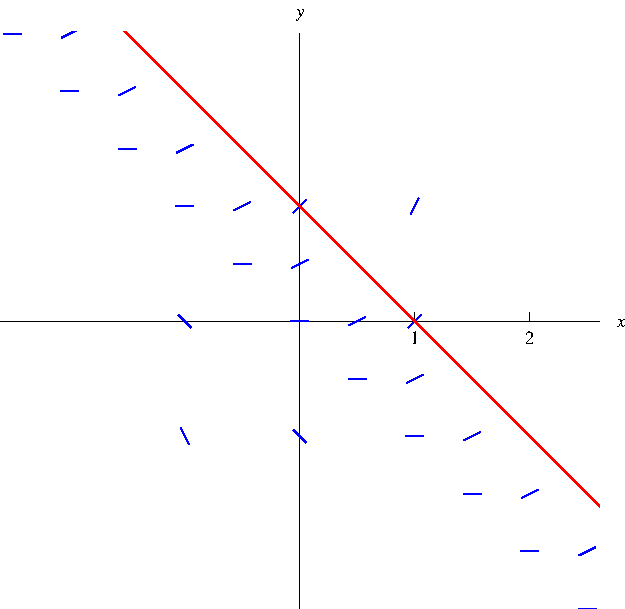
\includegraphics[height=5cm]{diff-eq-direction-fields/pictures/10-02-dirfieldx.pdf}%
}%
\only<handout:0| 28>{%
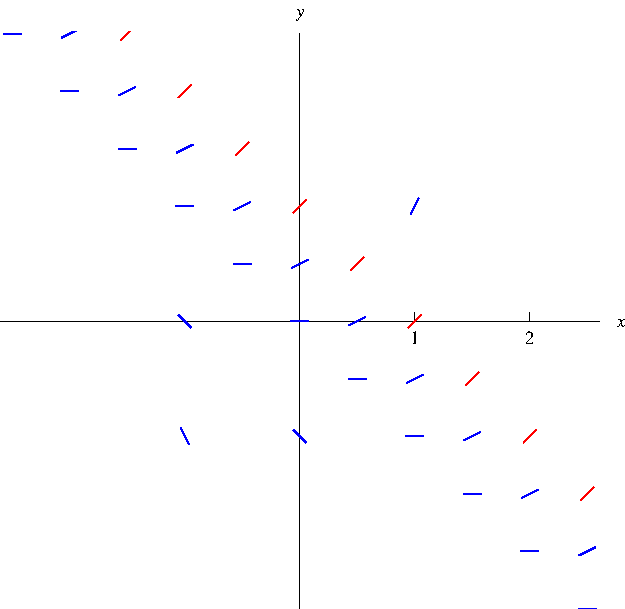
\includegraphics[height=5cm]{diff-eq-direction-fields/pictures/10-02-dirfieldy.pdf}%
}%
\only<handout:0| 29>{%
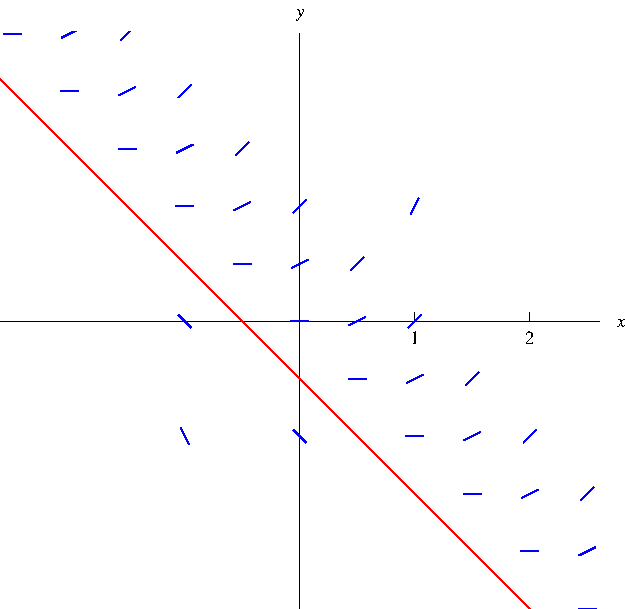
\includegraphics[height=5cm]{diff-eq-direction-fields/pictures/10-02-dirfieldz.pdf}%
}%
\only<handout:0| 30>{%
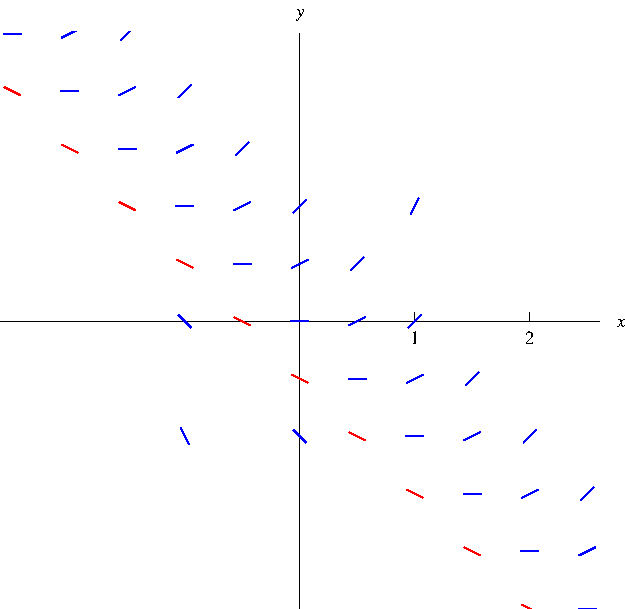
\includegraphics[height=5cm]{diff-eq-direction-fields/pictures/10-02-dirfieldaa.pdf}%
}%
\only<handout:0| 31>{%
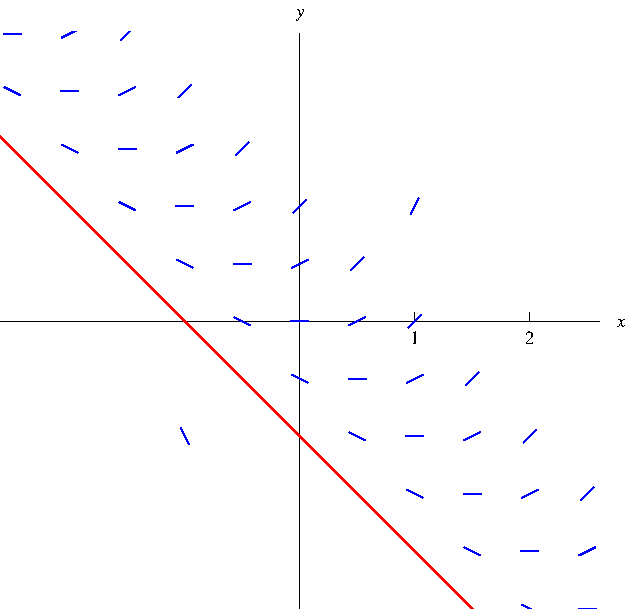
\includegraphics[height=5cm]{diff-eq-direction-fields/pictures/10-02-dirfieldab.pdf}%
}%
\only<handout:0| 32>{%
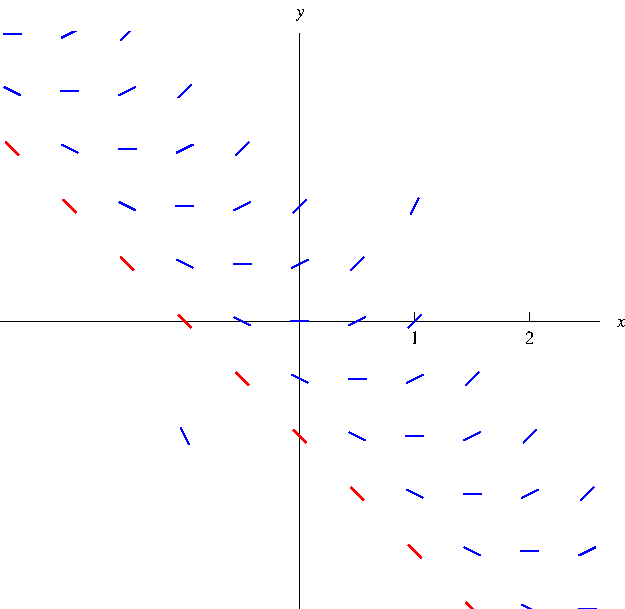
\includegraphics[height=5cm]{diff-eq-direction-fields/pictures/10-02-dirfieldac.pdf}%
}%
\only<handout:0| 33>{%
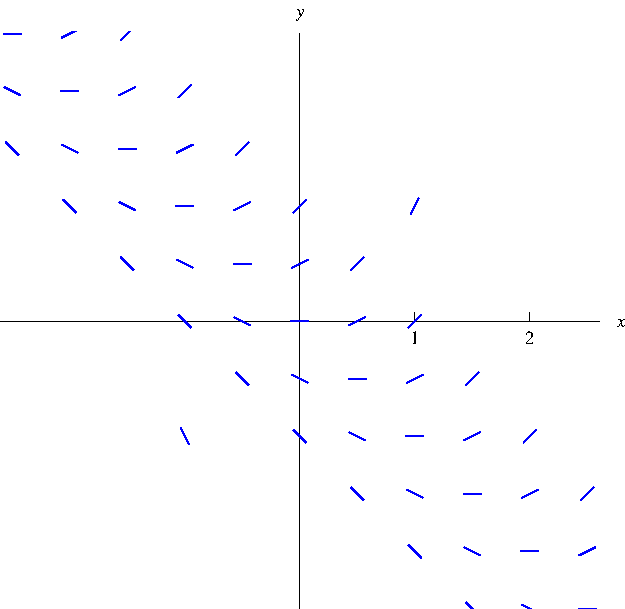
\includegraphics[height=5cm]{diff-eq-direction-fields/pictures/10-02-dirfieldad.pdf}%
}%
\only<handout:0| 34>{%
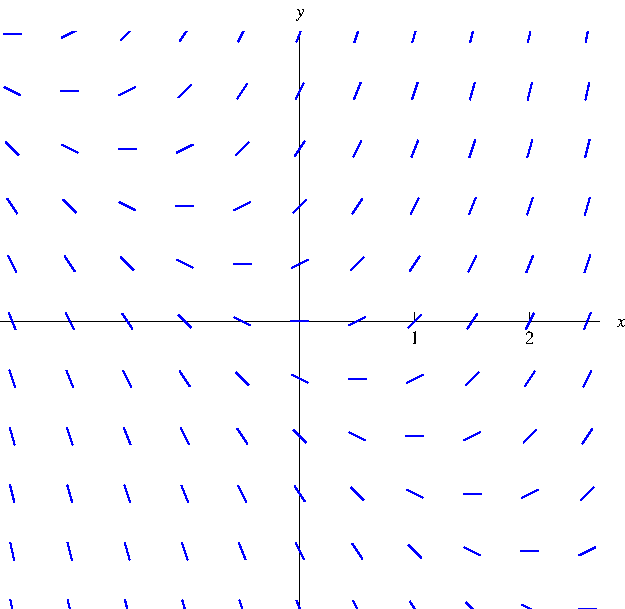
\includegraphics[height=5cm]{diff-eq-direction-fields/pictures/10-02-dirfieldae.pdf}%
}%
\only<35>{%
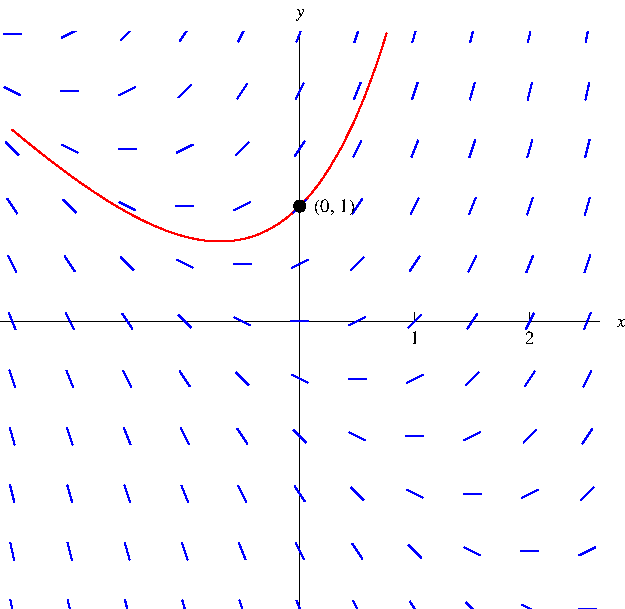
\includegraphics[height=5cm]{diff-eq-direction-fields/pictures/10-02-dirfieldaf.pdf}%
}%

\column{.3\textwidth}
\uncover<22->{%
\[%
\begin{array}{|l|r|}
\hline
\textrm{Line} & y' \\
\hline
\alert<handout:0| 23-24>{y = -x}&%
\alert<handout:0| 23-24>{\uncover<24->{0}}\\%
\alert<handout:0| 25-26>{y = -x+\frac{1}{2}}&%
\alert<handout:0| 25-26>{\uncover<26->{\frac{1}{2}}}\\%
\alert<handout:0| 27-28>{y = -x+1}&%
\alert<handout:0| 27-28>{\uncover<28->{1}}\\%
\alert<handout:0| 29-30>{y = -x-\frac{1}{2}}&%
\alert<handout:0| 29-30>{\uncover<30->{-\frac{1}{2}}}\\%
\alert<handout:0| 31-32>{y = -x-1}&%
\alert<handout:0| 31-32>{\uncover<32->{-1}}\\%
\hline
\end{array}
\]%
}%
\end{columns}
\end{frame}
% end module direction-fields-procedure

%% begin module diff-eq-natural-growth
\begin{frame}
\frametitle{Models of Population Growth}
\begin{itemize}
\item  One model for population growth assumes that the population grows at a rate proportional to its size.
\item  In other words, if a certain number of bacteria produce a certain number of offspring in a certain time, then ten times that many bacteria produce ten times that many offspring in the same time.
\item  This is plausible when the population has unlimited food and environment and no restrictions on its size.
\item<2->  Name the variables:
\uncover<2->{%
\begin{quote}
$t = $ time %(the independent variable)

$P = $ the number of individuals in the population %(the dependent variable)
\end{quote}
}%
\item<3->  The rate of growth is $\diff P/\diff t$.
\item<4->  Then ``rate of growth proportional to population size'' means
\end{itemize}
\uncover<4->{%
\[
\frac{\diff P}{\diff t} = k P
\]
where $k$ is the proportionality constant.
}%
\end{frame}
% end module diff-eq-natural-growth

%% begin module diff-eq-natural-growth-solution
\begin{frame}
\begin{columns}[c]
\column{.4\textwidth}
\[
\frac{\diff P}{\diff t} = k P
\]
\column{.6\textwidth}
\ \only<handout:0| -9>{%
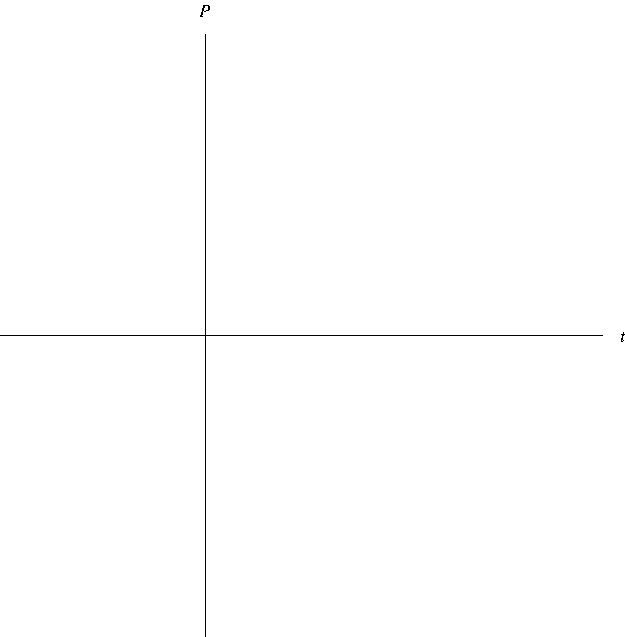
\includegraphics[height=4cm]{diff-eq-models/pictures/10-01-natgrowtha.pdf}%
}%
\only<handout:0| 10>{%
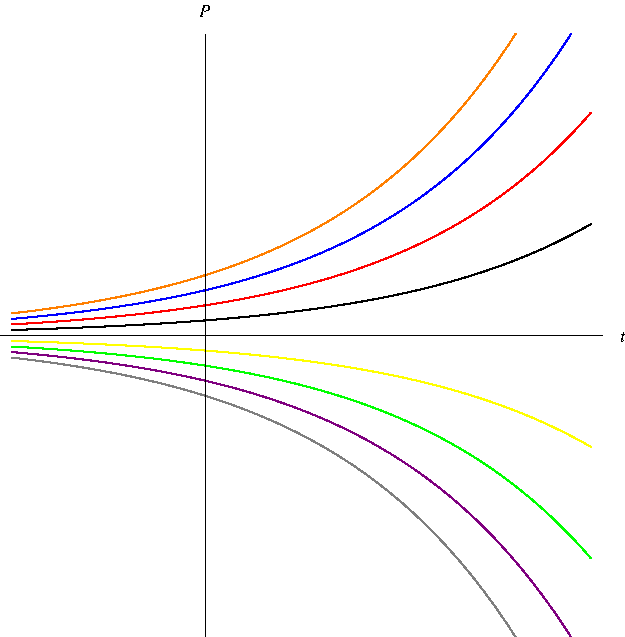
\includegraphics[height=4cm]{diff-eq-models/pictures/10-01-natgrowthb.pdf}%
}%
\only<11->{%
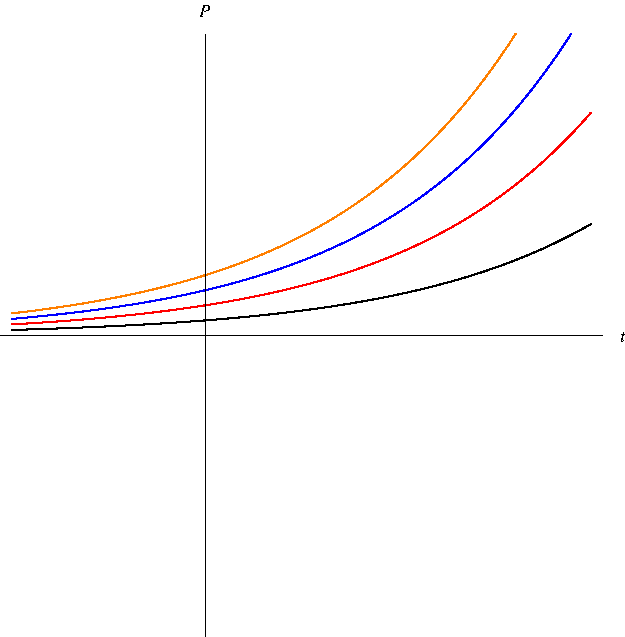
\includegraphics[height=4cm]{diff-eq-models/pictures/10-01-natgrowthc.pdf}%
}%
\end{columns}
\begin{itemize}
\item  This is a differential equation.
\item<2->  Exponential functions satisfy this condition.
\item<3->  Let $\alert<handout:0| 8>{P(t) = Ce^{kt}}$ ($C$ is a constant).  Then
\abovedisplayskip=0pt
\belowdisplayskip=0pt
\[
\uncover<4->{%
\frac{\diff P}{\diff t} = %
}%
\uncover<5->{%
\frac{\diff}{\diff t} (Ce^{kt}) = %
}%
\uncover<6->{%
 Cke^{kt} = %
}%
\uncover<7->{%
 k\alert<handout:0| 8>{Ce^{kt}} = %
}%
\uncover<8->{%
 k\alert<handout:0| 8>{P(t)} %
}%
\]
\item<9->  Therefore any function of the form $P(t) = Ce^{kt}$ satisfies the equation.  We will see later that there is no other solution.
\item<10->  Letting $C$ vary over the real numbers gives a family of solutions.
\item<11->  Populations have positive values, so we only care about $C > 0$.
\end{itemize}
\end{frame}
% end module diff-eq-natural-growth-solution

%% begin module diff-eq-logistic
\begin{frame}
\begin{itemize}
\item  This model works well under ideal conditions.
\item  In real life, most populations are constrained by the environment, the amount of food, etc.
\item  Many populations start by increasing exponentially, but then level off when they approach some upper bound, called the carrying capacity $K$.
\item<2->  To take this into account, make two assumptions:
\begin{itemize}
\item<2->  $\frac{\diff P}{\diff t} \approx kP$ if $P$ is small (Initially, the growth rate is proportional to $P$).
\item<2->  $\frac{\diff P}{\diff t} < 0$ if $P > K$ ($P$ decreases if it ever exceeds $K$).
\end{itemize}
\item<3->  Here is an expression that takes both assumptions into account:
\[
\uncover<3->{%
\frac{\diff P}{\diff t} = kP\left( 1 - \frac{P}{K}\right)
}%
\]
\item<4->  This is called the logistic differential equation.
\end{itemize}
\end{frame}
% end module diff-eq-logistic

%% begin module diff-eq-logistic-graph
\begin{frame}
\[
\frac{\diff P}{\diff t} = kP\left( 1 - \frac{P}{K}\right)
\]
\begin{itemize}
\item  What do the solutions look like?
\item<2->  $P = 0$ and $P = K$ are special solutions, called equilibrium solutions.
\item<3->  If $P > K$, then $1 - P/K < 0$ , so $\diff P/ \diff t < 0$, and $P$ decreases.
\item<4->  If $P < K$, then $1 - P/K > 0$, so $\diff P/\diff t > 0$, and $P$ increases.
\item<5->  As $P \rightarrow K$, $1 - P/K \rightarrow 0$, so $\diff P/\diff t \rightarrow 0$ and $P$ levels off.
\end{itemize}
%\begin{center}


\hfil \hfil\psset{xunit=0.8cm, yunit=0.8cm}
\begin{pspicture}(-2.000000, -0.700000)(3.200000,4) 
\tiny 
\psaxes[ticks=none, labels=none, arrows=<->](0, 0)(-2, -0.550000)(5.000000, 3.873671)
\rput[t](5.000000, -0.1){$t$}
\rput[r](-0.1,3.873671){$P$}

\uncover<2->{
\psline(-1.95, 1)( 5,1)
\rput[rt](-0.05, 0.95){$P=K$}
\rput[rt](-0.05, -0.05){$P=0$}
}

\uncover<3->{
%Function formula: \frac{3/2*e^{x}}{3/2*e^{x}-1/2} 
\psplot[linecolor=red, plotpoints=1000]{-0.800000}{5.000000}{2.718281828 x exp 1.5000000 mul -0.5000000 2.718281828 x exp 1.5000000 mul add div }

%Function formula: \frac{7/5*e^{x}}{7/5*e^{x}-2/5} 
\psplot[linecolor=purple, plotpoints=1000]{-0.9}{5.000000}{2.718281828 x exp 1.4000000 mul -0.4000000 2.718281828 x exp 1.4000000 mul add div }

%Function formula: \frac{13/10*e^{x}}{13/10*e^{x}-3/10} 
\psplot[linecolor=green, plotpoints=1000]{-1.100000}{5.000000}{2.718281828 x exp 1.3000000 mul -0.3000000 2.718281828 x exp 1.3000000 mul add div }

%Function formula: \frac{11/10*e^{x}}{11/10*e^{x}-1/10} 
\psplot[linecolor=brown, plotpoints=1000]{-1.95}{5.000000}{2.718281828 x exp 1.1000000 mul -0.1000000 2.718281828 x exp 1.1000000 mul add div }
}

\uncover<4->{
%Function formula: \frac{2/5*e^{x}}{2/5*e^{x}+3/5} 
\psplot[linecolor=orange, plotpoints=1000]{-1.95}{5.000000}{2.718281828 x exp 0.4000000 mul 0.6000000 2.718281828 x exp 0.4000000 mul add div }

%Function formula: \frac{3/10*e^{x}}{3/10*e^{x}+7/10} 
\psplot[linecolor=blue, plotpoints=1000]{-1.95}{5.000000}{2.718281828 x exp 0.3000000 mul 0.7000000 2.718281828 x exp 0.3000000 mul add div }

%Function formula: \frac{1/5*e^{x}}{1/5*e^{x}+4/5} 
\psplot[linecolor=red, plotpoints=1000]{-1.95}{5.000000}{2.718281828 x exp 0.2000000 mul 0.8000000 2.718281828 x exp 0.2000000 mul add div }

%Function formula: \frac{1/10*e^{x}}{1/10*e^{x}+9/10} 
\psplot[linecolor=cyan, plotpoints=1000]{-1.95}{5.000000}{2.718281828 x exp 0.1000000 mul 0.9000000 2.718281828 x exp 0.1000000 mul add div }
}
\end{pspicture} 

\end{frame}
% end module diff-eq-logistic-graph


%% begin module parametric-ex2
\begin{frame}
\begin{example} %[Example 2, p. 658]
Sketch and identify the curve defined by the parametric equations
\abovedisplayskip=2pt
\belowdisplayskip=2pt
\[
\alert<handout:0| 15>{x = \cos t}, \qquad \alert<handout:0| 14>{y = \sin t}.
\]
\begin{columns}[c]
\column{.55\textwidth}

\psset{xunit=2, yunit=2cm}
\begin{pspicture}(-1.5, -1.5)(1.5,1.5)

\tiny
\fcAxesStandard{-1.4}{-1.4}{1.4}{1.4}

\fcXTick{1}
\rput[rb](0.95, 0.05){$(1,0)$}

%Calculator input for full circle: plotCurve{}(\cos{}t, \sin{}t, 0, 2 \pi)
\uncover<handout:0| 3->{
\fcFullDot{1}{0}
\rput[bl](1.05, 0.05){$t=0$}
}

\uncover<handout:0| 5->{
\parametricplot[arrows=->, linecolor=\fcColorGraph, plotpoints=200] {0} {0.261799388}{t 57.29578 mul cos t 57.29578 mul sin }
\parametricplot[ linecolor=\fcColorGraph, plotpoints=200] {0.261799388} {0.523598776}{t 57.29578 mul cos t 57.29578 mul sin }
\rput[bl](0.9, 0.5){$t=\frac{\pi}{6}$}
\fcFullDot{0.866025} {0.500000}
}

\uncover<handout:0| 7->{
\tiny
%Calculator input: plotCurve{}(\cos{}t, \sin{}t, 1/4 \pi, 1/3 \pi)
\parametricplot[linecolor=\fcColorGraph, plotpoints=1000]{0.785398}{1.0472}{t 57.29578 mul cos t 57.29578 mul sin }
%Calculator input: plotCurve{}(\cos{}t, \sin{}t, 1/6 \pi, 1/4 \pi)
\parametricplot[arrows=->, linecolor=\fcColorGraph, plotpoints=1000]{0.523599}{0.785398}{t 57.29578 mul cos t 57.29578 mul sin }
\fcFullDot{0.500000}{0.866025}
\rput[bl](0.55, 0.9){$t=\frac{\pi}{3}$}
}
\uncover<handout:0| 9->{
%Calculator input: plotCurve{}(\cos{}t, \sin{}t, 5/12 \pi, 1/2 \pi)
\parametricplot[linecolor=\fcColorGraph, plotpoints=1000]{1.309}{1.5708}{t 57.29578 mul cos t 57.29578 mul sin }
%Calculator input: plotCurve{}(\cos{}t, \sin{}t, 1/3 \pi, 5/12 \pi)
\parametricplot[arrows=->, linecolor=\fcColorGraph, plotpoints=1000]{1.0472}{1.309}{t 57.29578 mul cos t 57.29578 mul sin }
\fcFullDot{0.000000}{ 1.000000}
\rput[bl](0.1, 1.05){$t=\frac{\pi}{2}$}
}
\uncover<handout:0| 11->{
%Calculator input: plotCurve{}(\cos{}t, \sin{}t, 3/4 \pi, \pi)
\parametricplot[linecolor=\fcColorGraph, plotpoints=1000]{2.35619}{3.14159}{t 57.29578 mul cos t 57.29578 mul sin }
%Calculator input: plotCurve{}(\cos{}t, \sin{}t, 1/2 \pi, 3/4 \pi)
\parametricplot[arrows=->, linecolor=\fcColorGraph, plotpoints=1000]{1.5708}{2.35619}{t 57.29578 mul cos t 57.29578 mul sin }
\fcFullDot{-1}{0}
\rput[rb](-1, 0.1){$t=\pi$}
}
\uncover<handout:0| 13->{
%Calculator input: plotCurve{}(\cos{}t, \sin{}t, 5/4 \pi, 3/2 \pi)
\parametricplot[linecolor=\fcColorGraph, plotpoints=1000]{3.92699}{4.71239}{t 57.29578 mul cos t 57.29578 mul sin }
%Calculator input: plotCurve{}(\cos{}t, \sin{}t, \pi, 5/4 \pi)
\parametricplot[arrows=->, linecolor=\fcColorGraph, plotpoints=1000]{ 3.14159} {3.92699}{t 57.29578 mul cos t 57.29578 mul sin }
\fcFullDot{0}{-1}
\rput[tr](-0.1, -1.05){$t=\frac{3\pi}{2}$}
}
\uncover<handout:0| 15->{
%Calculator input: plotCurve{}(\cos{}t, \sin{}t, 7/4 \pi, 2 \pi)
\parametricplot[linecolor=\fcColorGraph, plotpoints=1000 ]{ 5.49779}{6.28319}{t 57.29578 mul cos t 57.29578 mul sin }
%Calculator input: plotCurve{}(\cos{}t, \sin{}t, 3/2 \pi, 7/4 \pi)
\parametricplot[arrows=->, linecolor=\fcColorGraph, plotpoints=1000]{4.71239}{5.49779}{t 57.29578 mul cos t 57.29578 mul sin }
\rput[tl](1, -0.1){$t=2\pi$}
}
\end{pspicture}

%\ \only<handout:0| -2>{%
%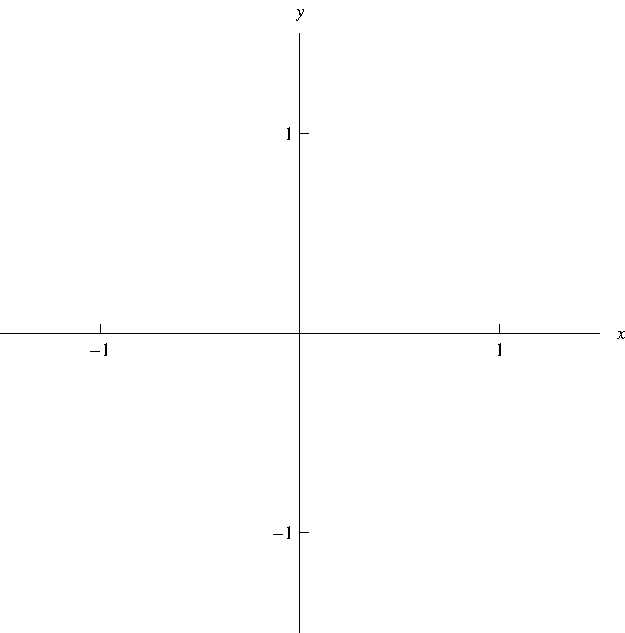
\includegraphics[height=6cm]{parametric-curves/pictures/11-01-ex2a.pdf}%
%}%
%\only<handout:0| 3-4>{%
%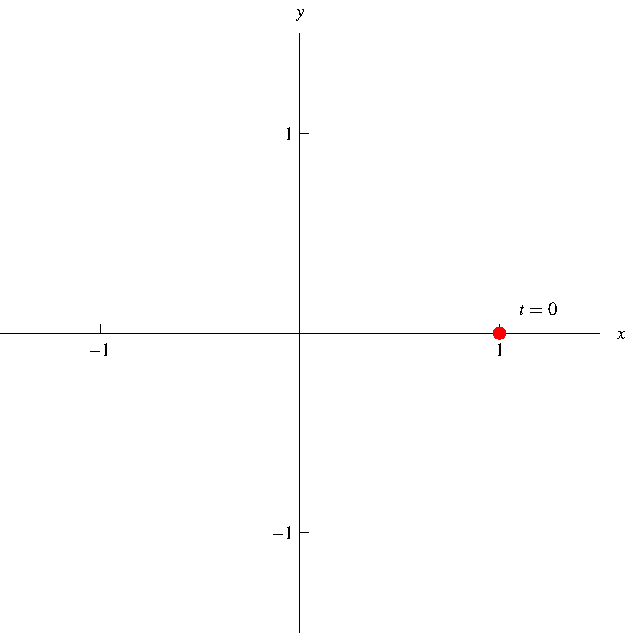
\includegraphics[height=6cm]{parametric-curves/pictures/11-01-ex2b.pdf}%
%}%
%\only<handout:0| 5-6>{%
%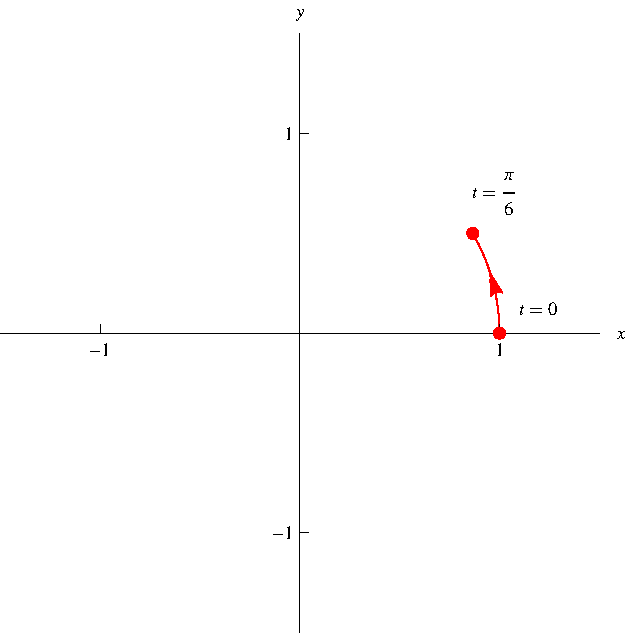
\includegraphics[height=6cm]{parametric-curves/pictures/11-01-ex2c.pdf}%
%}%
%\only<handout:0| 7-8>{%
%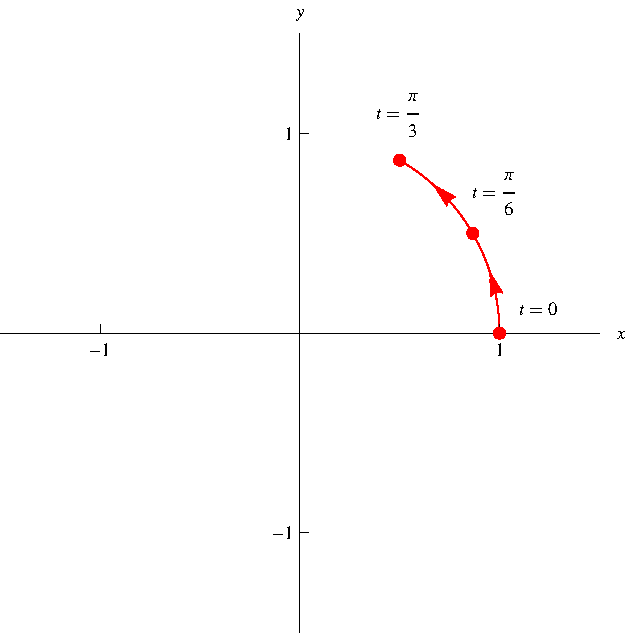
\includegraphics[height=6cm]{parametric-curves/pictures/11-01-ex2d.pdf}%
%}%
%\only<handout:0| 9-10>{%
%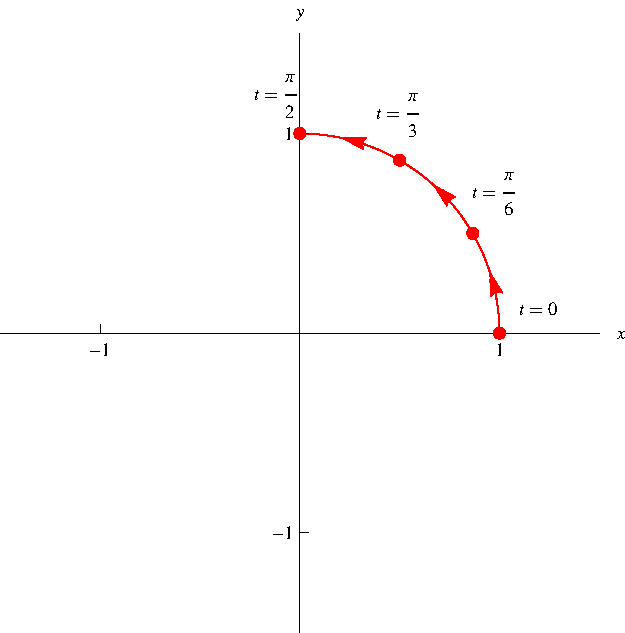
\includegraphics[height=6cm]{parametric-curves/pictures/11-01-ex2e.pdf}%
%}%
%\only<handout:0| 11-12>{%
%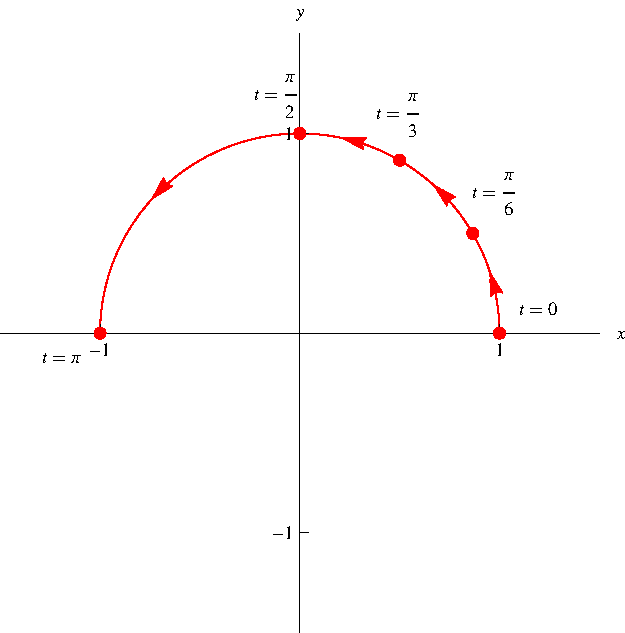
\includegraphics[height=6cm]{parametric-curves/pictures/11-01-ex2f.pdf}%
%}%
%\only<handout:0| 13-14>{%
%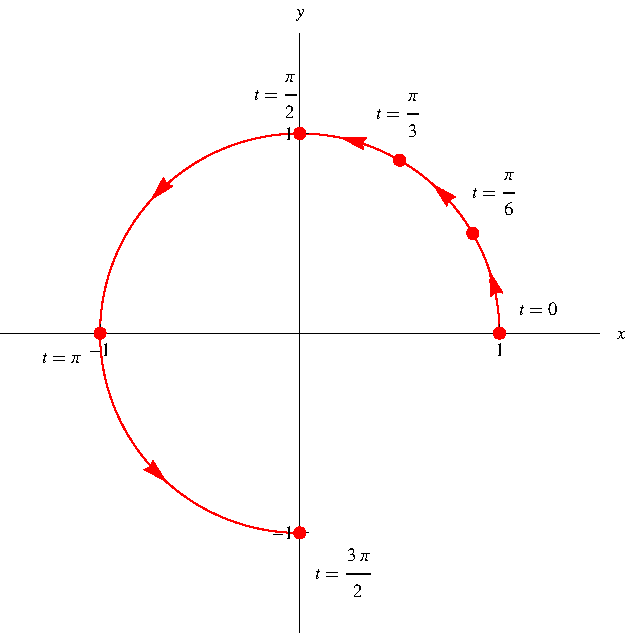
\includegraphics[height=6cm]{parametric-curves/pictures/11-01-ex2g.pdf}%
%}%
%\only<15->{%
%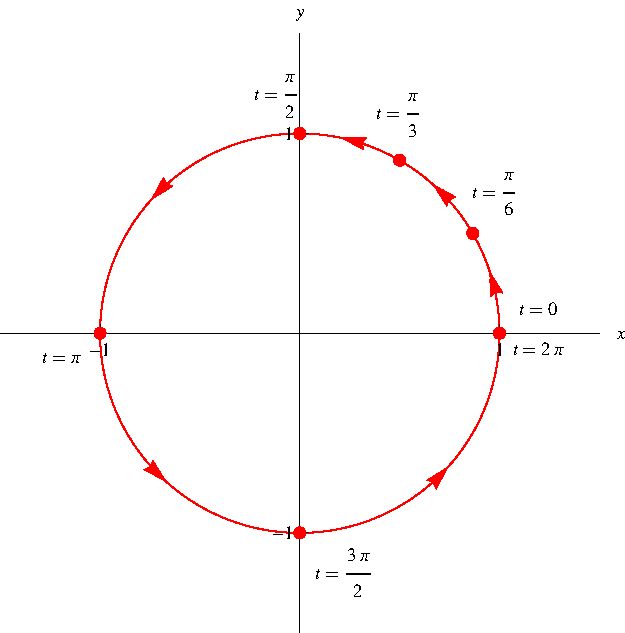
\includegraphics[height=6cm]{parametric-curves/pictures/11-01-ex2h.pdf}%
%}%

\column{.45\textwidth}
\[
\begin{array}{|r|r|r|}
\hline
t & x & y\\
\hline
\alert<handout:0| 2-3>{0} &%
\alert<handout:0| 2-3>{\uncover<3->{1}} &%
\alert<handout:0| 2-3>{\uncover<3->{0}} \\%
\alert<handout:0| 4-5>{\frac{\pi}6} &%
\alert<handout:0| 4-5>{\uncover<5->{\frac{\sqrt{3}}{2}}} &%
\alert<handout:0| 4-5>{\uncover<5->{\frac12}} \\%
\alert<handout:0| 6-7>{\frac{\pi}3} &%
\alert<handout:0| 6-7>{\uncover<7->{\frac12}} &%
\alert<handout:0| 6-7>{\uncover<7->{\frac{\sqrt{3}}2}} \\%
\alert<handout:0| 8-9>{\frac{\pi}2} &%
\alert<handout:0| 8-9>{\uncover<9->{0}} &%
\alert<handout:0| 8-9>{\uncover<9->{1}} \\%
\alert<handout:0| 10-11>{\pi} &%
\alert<handout:0| 10-11>{\uncover<11->{-1}} &%
\alert<handout:0| 10-11>{\uncover<11->{0}} \\%
\alert<handout:0| 12-13>{\frac{3\pi}2} &%
\alert<handout:0| 12-13>{\uncover<13->{0}} &%
\alert<handout:0| 12-13>{\uncover<13->{-1}} \\%
\alert<handout:0| 14-15>{2\pi} &%
\alert<handout:0| 14-15>{\uncover<15->{1}} &%
\alert<handout:0| 14-15>{\uncover<15->{0}} \\%
\hline
\end{array}
\]
\abovedisplayskip=2pt
\belowdisplayskip=2pt
\[
\uncover<16->{%
x^2 + y^2 = %
}%
\uncover<17->{%
\cos^2 t+ \sin^2 t = %
}%
\uncover<18->{%
1%
}%
\]
\uncover<19->{%
Therefore $(x,y)$ travels on the unit circle $x^2 + y^2 = 1$.
}%
\end{columns}
\end{example}
\end{frame}
% end module parametric-ex2

%% begin module polar-curve-ex4
\begin{frame}
\begin{example} %[Example 4, p. 677]
What curve is represented by the polar equation $r = 2$?
\begin{columns}[c]
\column{.5\textwidth}

\psset{xunit=0.5cm, yunit=0.5cm}
\begin{pspicture}(-4.8, -4.8)(4.8,4.8) 
\tiny 
\psframe*[linecolor=white](-4.8, -4.8)(4.8, 4.8)
%Force a bounding box for pdflatex:
\psline[linecolor=red!1](4.6, 4.6)(4.6001,4.6)
\psline[linecolor=red!1](-4.6, -4.6)(-4.6001,-4.6)
%
\psFullDotBlue{0}{0}
\psline{->}(0,0)(4.4)
\uncover<3->{
\rput[bl](1.5, 1.7){\alert<3>{$r=2$}}
}
\uncover<3>{
%Calculator input: plotCurve{}(2 \cos{}t, 2 \sin{}t, - \pi, \pi)
\parametricplot[linecolor=\psColorGraph, plotpoints=1000]{-3.14159}{3.14159}{t 57.29578 mul cos 2.0000000 mul t 57.29578 mul sin 2.0000000 mul }
}
\uncover<4->{
%Calculator input: plotCurve{}(2 \cos{}t, 2 \sin{}t, - \pi, \pi)
\parametricplot[plotpoints=1000]{-3.14159}{3.14159}{t 57.29578 mul cos 2.0000000 mul t 57.29578 mul sin 2.0000000 mul }
}
\uncover<4->{
\rput[bl](0.6, 0.88){\alert<4>{$r=1$}}
}
\uncover<4>{
\parametricplot[linecolor=\psColorGraph, plotpoints=1000]{-3.14159}{3.14159}{t 57.29578 mul cos t 57.29578 mul sin  }
}
\uncover<5->{
\parametricplot[plotpoints=1000]{-3.14159}{3.14159}{t 57.29578 mul cos t 57.29578 mul sin  }
}
\uncover<5->{
\rput[bl](3.2, 3.4){\alert<5>{$r=4$}}
}
\uncover<5>{
\parametricplot[linecolor=\psColorGraph, plotpoints=1000]{-3.14159}{3.14159}{t 57.29578 mul cos 4 mul t 57.29578 mul sin 4 mul }
}
\end{pspicture}
%\only<handout:0| -2>{%
%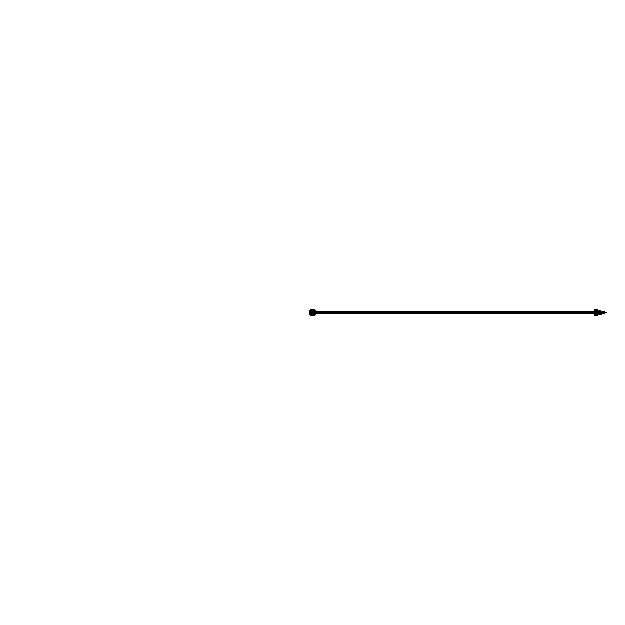
\includegraphics[height=6cm]{polar-curves/pictures/11-03-ex4a.pdf}%
%}%
%\only<handout:0| 3>{%
%\includegraphics[height=6cm]{polar-curves/pictures/11-03-ex4b.pdf}%
%}%
%\only<handout:0| 4>{%
%\includegraphics[height=6cm]{polar-curves/pictures/11-03-ex4c.pdf}%
%}%
%\only<5->{%
%\includegraphics[height=6cm]{polar-curves/pictures/11-03-ex4d.pdf}%
%}%
\column{.5\textwidth}
\begin{itemize}
\item<2->  The equation describes all points that are $2$ units away from $O$.
\item<3->  This is the circle with center $O$ and radius $2$.
\item<4->  The equation $r = 1$ describes the unit circle.
\item<5->  The equation $r = 4$ describes the circle with center $O$ and radius $4$.
\end{itemize}
\end{columns}
\end{example}
\end{frame}
% end module polar-curve-ex4

%% begin module polar-curve-ex6
\begin{frame}[t]
\begin{example} %[Example 6, p. 678]
\begin{enumerate}
\item<1-| alert@2-21> Sketch the curve with polar equation \alertNoH{ 26}{$r = 2\cos \theta$}.
\item<1-| alert@22-> Find a Cartesian equation for this curve.
\end{enumerate}
\begin{columns}[c]
\column{.5\textwidth}
\psset{xunit=1.75cm, yunit=1.75cm}
\begin{pspicture}(-0.6, -1.5)(2.5,1.5)

\tiny
\fcAxesStandard{-0.52}{-1.4}{2.4}{1.4}

\uncover<21->{
%Calculator input: plotCurve{}(2 \cos^{2}{}t, 2 \cos{}t \sin{}t, 0, 2 \pi)
\parametricplot[linecolor=\fcColorGraph, plotpoints=200]{0}{6.28319}{t 57.29578 mul cos 2.0000000 exp 2.0000000 mul t 57.29578 mul sin t 57.29578 mul cos mul 2.0000000 mul }
}
\uncover<4->{
\fcFullDot{2}{0}
\rput[bl](2.05,0.05){$(2,0)$}
}
\uncover<6->{
\fcFullDot{1.500000}{0.866025}
\rput[bl](1.55,0.9){$\left(\sqrt{3}, \frac{\pi}{6}\right)$}
}

\uncover<8->{
\fcFullDot{1}{1}
\rput[bl](1.05,1.05){$\left(\sqrt{2}, \frac{\pi}{4}\right)$}
}
\uncover<10->{
\fcFullDot{0.5}{0.866025}
\rput[br](0.45,0.86){$\left(1, \frac{\pi}{3}\right)$}
}
\uncover<12->{
\fcFullDot{0}{0}
\rput[tr](-0.05,-0.05){$\left(0,\frac{\pi}{2}\right)$}
}
\uncover<14->{
\fcFullDot{0.5}{ -0.866025}
\rput[t](0.5,-0.88){$\left(-1, \frac{2\pi}{3}\right)$}
}
\uncover<16->{
\fcFullDot{1}{-1}
\rput[t](1,-1.05){$\left(-\sqrt{2},\frac{3\pi}{4}\right)$}
}
\uncover<18->{
\fcFullDot{1.5}{-0.866025}
\rput[lt](1.5,-0.9){$\left(-\sqrt{3},\frac{5\pi}{6}\right)$}
}
\uncover<4-5>{
\psline[linecolor=blue](0,0)(2,0)
}
\uncover<6-7>{
\parametricplot[arrows=->, linecolor=\fcColorGraph, plotpoints=200] {0}{0.523598776 }{t 57.29578 mul cos 0.3 mul t 57.29578 mul sin 0.3 mul }
\psline[linecolor=blue](0,0)(1.5,0.866025)
}
\uncover<8-9>{
\parametricplot[arrows=->, linecolor=\fcColorGraph, plotpoints=200] {0}{0.785398163}{t 57.29578 mul cos 0.3 mul t 57.29578 mul sin 0.3 mul }
\psline[linecolor=blue](0,0)(1,1)
}
\uncover<10-11>{
\parametricplot[arrows=->, linecolor=\fcColorGraph, plotpoints=200] {0}{1.047197551}{t 57.29578 mul cos 0.3 mul t 57.29578 mul sin 0.3 mul }
\psline[linecolor=blue](0,0)(0.5,0.866025)
}
\uncover<12-13>{
\parametricplot[arrows=->, linecolor=\fcColorGraph, plotpoints=200] {0}{1.570796327}{t 57.29578 mul cos 0.3 mul t 57.29578 mul sin 0.3 mul }
}
\uncover<14-15>{
\parametricplot[arrows=->, linecolor=\fcColorGraph, plotpoints=200] {0}{2.094395102}{t 57.29578 mul cos 0.3 mul t 57.29578 mul sin 0.3 mul }
\psline[linecolor=blue](0,0)(0.5, -0.866025)
\psline[linecolor=blue, linestyle=dashed](0,0)(-0.500000, 0.866025)
}
\uncover<16-17>{
\parametricplot[arrows=->, linecolor=\fcColorGraph, plotpoints=200] {0}{2.35619449}{t 57.29578 mul cos 0.3 mul t 57.29578 mul sin 0.3 mul }
\psline[linecolor=blue, linestyle=dashed](0,0)(-0.5, 0.5)
\psline[linecolor=blue](0,0)(1, -1)
}
\uncover<18-19>{
\parametricplot[arrows=->, linecolor=\fcColorGraph, plotpoints=200] {0}{2.617993878}{t 57.29578 mul cos 0.3 mul t 57.29578 mul sin 0.3 mul }
\psline[linecolor=blue, linestyle=dashed](0,0)(-0.500000, 0.288675)
\psline[linecolor=blue](0,0)(1.500000, -0.866025)
}
\uncover<20>{
\parametricplot[arrows=->, linecolor=\fcColorGraph, plotpoints=200] {0}{3.141592654}{t 57.29578 mul cos 0.3 mul t 57.29578 mul sin 0.3 mul }
\psline[linecolor=blue, linestyle=dashed](0,0)(-0.5,0)
\psline[linecolor=blue](0,0)(2,0)
}
\end{pspicture}
\vspace{1cm}
%\ \only<handout:0| -3>{%
%\includegraphics[height=6cm]{polar-curves/pictures/11-03-ex6z.pdf}%
%}%
%\only<handout:0| 4-5>{%
%\includegraphics[height=6cm]{polar-curves/pictures/11-03-ex6a.pdf}%
%}%
%\only<handout:0| 6-7>{%
%\includegraphics[height=6cm]{polar-curves/pictures/11-03-ex6b.pdf}%
%}%
%\only<handout:0| 8-9>{%
%\includegraphics[height=6cm]{polar-curves/pictures/11-03-ex6c.pdf}%
%}%
%\only<handout:0| 10-11>{%
%\includegraphics[height=6cm]{polar-curves/pictures/11-03-ex6d.pdf}%
%}%
%\only<handout:0| 12-13>{%
%\includegraphics[height=6cm]{polar-curves/pictures/11-03-ex6e.pdf}%
%}%
%\only<handout:0| 14-15>{%
%\includegraphics[height=6cm]{polar-curves/pictures/11-03-ex6f.pdf}%
%}%
%\only<handout:0| 16-17>{%
%\includegraphics[height=6cm]{polar-curves/pictures/11-03-ex6g.pdf}%
%}%
%\only<handout:0| 18-19>{%
%\includegraphics[height=6cm]{polar-curves/pictures/11-03-ex6h.pdf}%
%}%
%\only<handout:0| 20>{%
%\includegraphics[height=6cm]{polar-curves/pictures/11-03-ex6i.pdf}%
%}%
%\only<21->{%
%\includegraphics[height=6cm]{polar-curves/pictures/11-03-ex6j.pdf}%
%}%
\column{.5\textwidth}
\only<handout:1| -21>{\uncover<2->{%
\[
\begin{array}{|@{\ }l@{\ }|r@{\ }|}
\hline
\theta & r \\
\hline
\alertNoH{ 3-4}{%
0%
}&%
\uncover<4->{\alertNoH{ 4}{%%
2%
}}\\%%
\alertNoH{ 5-6}{%
\pi /6%
}&%
\uncover<6->{\alertNoH{ 6}{%%
\sqrt{3}%
}}\\%%
\alertNoH{ 7-8}{%
\pi /4%
}&%
\uncover<8->{\alertNoH{ 8}{%%
\sqrt{2}%
}}\\%%
\alertNoH{ 9-10}{%
\pi /3%
}&%
\uncover<10->{\alertNoH{ 10}{%%
1%
}}\\%%
\alertNoH{ 11-12}{%
\pi /2%
}&%
\uncover<12->{\alertNoH{ 12}{%%
0%
}}\\%%
\alertNoH{ 13-14}{%
2\pi /3%
}&%
\uncover<14->{\alertNoH{ 14}{%%
-1%
}}\\%%
\alertNoH{ 15-16}{%
3\pi /4%
}&%
\uncover<16->{\alertNoH{ 16}{%%
-\sqrt{2}%
}}\\%%
\alertNoH{ 17-18}{%
5\pi /6%
}&%
\uncover<18->{\alertNoH{ 18}{%%
-\sqrt{3}%
}}\\%%
\alertNoH{ 19-20}{%
\pi%
}&%
\uncover<20->{\alertNoH{ 20}{%%
-2%
}}\\%%
\hline
\end{array}
\]
}}%
\only<handout:2| 22->{%
\begin{itemize}
\item<22-| alert@22-23>  $x = $ \uncover<23->{$r\cos \theta$.}
\item<24-| alert@24-25>  $\cos \theta = $ \uncover<25->{$x/r$.}
\item<26-| alert@26-27>  $r = 2\cos \theta = $ \uncover<27->{$\alertNoH{ 28}{2x}/r$.}
\item<28-| alert@28-30>  $2x = $ \uncover<29->{$r^2 = $ \uncover<30->{$x^2+y^2$.}}
\item<31->  $x^2 + y^2 - 2x = 0$.
\item<32->  Complete the square:
\end{itemize}
\begin{eqnarray*}
\uncover<32->{%
(x^2 - 2x \uncover<33->{\alertNoH{ 33}{+ 1}}) + y^2%
}%
& \uncover<32->{ = } &%
\uncover<32->{%
0 \uncover<33->{\alertNoH{ 33}{+ 1}}%
}\\%
\uncover<34->{%
(x-1)^2 + y^2%
}%
& \uncover<34->{ = } &%
\uncover<34->{%
1%
}%
\end{eqnarray*}
}%
\end{columns}
\end{example}
\end{frame}
% end module polar-curve-ex6

%% begin module cardioid-ex7
\begin{frame}
\begin{example} %[Example 7, p. 679]
Sketch the curve $r = 1 + \sin \theta$.
\begin{columns}[c]
\column{.3\textwidth}
\psset{xunit=1cm, yunit=1cm}
\begin{pspicture}(-1.499038, -0.700000)(1.6,2.4) 

\tiny 
\psaxesStandard{-1.4}{-0.6}{1.4}{2.3}
\psLabelXOne
\psLabelYOne
\uncover<2-6>{
%Calculator input: plotCurve{}(\cos{}t \sin{}t+\cos{}t, \sin^{2}{}t+\sin{}t, 0, 2 \pi)
\parametricplot[arrows=->, linecolor=\psColorGraph, plotpoints=200] {0}{0.7}{t 57.29578 mul cos t 57.29578 mul sin t 57.29578 mul cos mul add t 57.29578 mul sin t 57.29578 mul sin 2.0000000 exp add }
%Calculator input: plotCurve{}(\cos{}t \sin{}t+\cos{}t, \sin^{2}{}t+\sin{}t, 0, 2 \pi)
\parametricplot[linecolor=\psColorGraph, plotpoints=200] {0.7}{1.570796327} {t 57.29578 mul cos t 57.29578 mul sin t 57.29578 mul cos mul add t 57.29578 mul sin t 57.29578 mul sin 2.0000000 exp add }
}
%\uncover<3-6>{%
%\psFullDot{1.207107}{1.207107}
%}
\uncover<handout:0| 3>{%
\psline[linecolor=blue](0,0)(1.207107, 1.207107)
\psAngle{0}{0.785398}{0.4}{$\theta$}
\rput[b](0.6, 0.68){$r$}
} 
%\uncover<4-6>{%
%\psFullDot{1.017510}{1.522811}
%}
\uncover<handout:0| 4>{%
\psline[linecolor=blue](0,0)(1.017510, 1.522811)
\psAngle{0}{0.981748}{0.4}{$\theta$}
\rput[b](0.45, 0.8){$r$}
}
%\uncover<5-6>{%
%\psFullDot{0.736237}{1.777433}
%}
\uncover<handout:0| 5>{
\psline[linecolor=blue](0,0)(0.736237, 1.777433)
\psAngle{0}{1.178097}{0.4}{$\theta$}
\rput[b](0.3, 0.9){$r$}
}
%\uncover<6>{%
%\psFullDot{0.386432}{1.942725}
%} 
\uncover<handout:0| 6>{
\psAngle{0}{1.374447}{0.4}{$\theta$}
\psline[linecolor=blue](0,0)(0.386432, 1.942725)
\rput[b](0.1, 1.1){$r$}
} 
\uncover<handout:0| 7->{
%Calculator input: plotCurve{}(\cos{}t \sin{}t+\cos{}t, \sin^{2}{}t+\sin{}t, 0, 2 \pi)
\parametricplot[plotpoints=400, linecolor=blue] {0}{1.570796327}{t 57.29578 mul cos t 57.29578 mul sin t 57.29578 mul cos mul add t 57.29578 mul sin t 57.29578 mul sin 2.0000000 exp add }
}

\uncover<7>{
%Calculator input: plotCurve{}(\cos{}t \sin{}t+\cos{}t, \sin^{2}{}t+\sin{}t, 0, 2 \pi)
\parametricplot[arrows=->, linecolor=\psColorGraph, plotpoints=200] {1.570796327}{2.35619449}{t 57.29578 mul cos t 57.29578 mul sin t 57.29578 mul cos mul add t 57.29578 mul sin t 57.29578 mul sin 2.0000000 exp add }
%Calculator input: plotCurve{}(\cos{}t \sin{}t+\cos{}t, \sin^{2}{}t+\sin{}t, 0, 2 \pi)
\parametricplot[linecolor=\psColorGraph, plotpoints=200] {2.35619449}{3.141592654} {t 57.29578 mul cos t 57.29578 mul sin t 57.29578 mul cos mul add t 57.29578 mul sin t 57.29578 mul sin 2.0000000 exp add }
}
\uncover<handout:0| 8->{
%Calculator input: plotCurve{}(\cos{}t \sin{}t+\cos{}t, \sin^{2}{}t+\sin{}t, 0, 2 \pi)
\parametricplot[linecolor=blue, plotpoints=200] {1.570796327}{3.141592654} {t 57.29578 mul cos t 57.29578 mul sin t 57.29578 mul cos mul add t 57.29578 mul sin t 57.29578 mul sin 2.0000000 exp add }
}
\uncover<8>{
%Calculator input: plotCurve{}(\cos{}t \sin{}t+\cos{}t, \sin^{2}{}t+\sin{}t, 0, 2 \pi)
\parametricplot[arrows=->, linecolor=\psColorGraph, plotpoints=200] {3.141592654}{3.926990817}{t 57.29578 mul cos t 57.29578 mul sin t 57.29578 mul cos mul add t 57.29578 mul sin t 57.29578 mul sin 2.0000000 exp add }
%Calculator input: plotCurve{}(\cos{}t \sin{}t+\cos{}t, \sin^{2}{}t+\sin{}t, 0, 2 \pi)
\parametricplot[linecolor=\psColorGraph, plotpoints=200] {3.926990817}{4.71238898} {t 57.29578 mul cos t 57.29578 mul sin t 57.29578 mul cos mul add t 57.29578 mul sin t 57.29578 mul sin 2.0000000 exp add }
}
\uncover<handout:0| 9->{
%Calculator input: plotCurve{}(\cos{}t \sin{}t+\cos{}t, \sin^{2}{}t+\sin{}t, 0, 2 \pi)
\parametricplot[linecolor=blue, plotpoints=200] {3.141592654}{4.71238898} {t 57.29578 mul cos t 57.29578 mul sin t 57.29578 mul cos mul add t 57.29578 mul sin t 57.29578 mul sin 2.0000000 exp add }
}
\uncover<9>{
%Calculator input: plotCurve{}(\cos{}t \sin{}t+\cos{}t, \sin^{2}{}t+\sin{}t, 0, 2 \pi)
\parametricplot[arrows=->, linecolor=\psColorGraph, plotpoints=200] {4.71238898}{5.7}{t 57.29578 mul cos t 57.29578 mul sin t 57.29578 mul cos mul add t 57.29578 mul sin t 57.29578 mul sin 2.0000000 exp add }
%Calculator input: plotCurve{}(\cos{}t \sin{}t+\cos{}t, \sin^{2}{}t+\sin{}t, 0, 2 \pi)
\parametricplot[linecolor=\psColorGraph, plotpoints=200] {5.7}{6.283185307} {t 57.29578 mul cos t 57.29578 mul sin t 57.29578 mul cos mul add t 57.29578 mul sin t 57.29578 mul sin 2.0000000 exp add }
}
\uncover<handout:0| 10->{
%Calculator input: plotCurve{}(\cos{}t \sin{}t+\cos{}t, \sin^{2}{}t+\sin{}t, 0, 2 \pi)
\parametricplot[linecolor=blue, plotpoints=200] {4.71238898}{6.283185307} {t 57.29578 mul cos t 57.29578 mul sin t 57.29578 mul cos mul add t 57.29578 mul sin t 57.29578 mul sin 2.0000000 exp add }
}

\end{pspicture} 

%\ \only<handout:0| 1>{%
%\includegraphics[height=3.6cm]{polar-curves/pictures/11-03-ex7a.pdf}%
%}%
%\only<handout:0| 2>{%
%\includegraphics[height=3.6cm]{polar-curves/pictures/11-03-ex7b.pdf}%
%}%
%\only<handout:0| 3>{%
%\includegraphics[height=3.6cm]{polar-curves/pictures/11-03-ex7ba.pdf}%
%}%
%\only<handout:0| 4>{%
%\includegraphics[height=3.6cm]{polar-curves/pictures/11-03-ex7bb.pdf}%
%}%
%\only<handout:0| 5>{%
%\includegraphics[height=3.6cm]{polar-curves/pictures/11-03-ex7bc.pdf}%
%}%
%\only<handout:0| 6>{%
%\includegraphics[height=3.6cm]{polar-curves/pictures/11-03-ex7bd.pdf}%
%}%
%\only<handout:0| 7>{%
%\includegraphics[height=3.6cm]{polar-curves/pictures/11-03-ex7c.pdf}%
%}%
%\only<handout:0| 8>{%
%\includegraphics[height=3.6cm]{polar-curves/pictures/11-03-ex7d.pdf}%
%}%
%\only<9->{%
%\includegraphics[height=3.6cm]{polar-curves/pictures/11-03-ex7e.pdf}%
%}%
\column{.7\textwidth}
\psset{xunit=1cm, yunit=1cm}
\begin{pspicture}(-0.700000, -0.700000)(6.55,2.4) 

\tiny 
\psframe*[linecolor=white](-0.7, -0.7)(6.55, 2.4)
\psaxes[arrows=<->, Dx=1.570796327, Dy=1, labels=none](0,0)(-0.5, -0.5)(6.4, 2.3)
\rput[r](-0.1,2.3){$r$}
\rput[t](6.48,-0.01){$\theta$}
\rput[r](-0.15,1){$1$}
\rput[r](-0.15,2){$2$}

\rput[t](! 1.570796327 -0.15){$\frac{\pi}2$}
\rput[t](! 1.570796327 2 mul -0.15){$\pi$}
\rput[t](! 1.570796327 3 mul -0.15){$\frac{3\pi}{2}$}
\rput[t](! 1.570796327 4 mul -0.15){$2\pi$}

\rput[l](3.4, 1){$r=1+\sin \theta$}

\uncover<handout:0| 3>{
\psLengthIndicator{0}{-0.1}{0.785398163}{-0.1}{$\theta$}
\psline[linecolor=blue](0.785398163, 0)(0.785398163, 1.707107)
}
\uncover<handout:0| 4>{
\psLengthIndicator{0}{-0.1}{0.981747704}{-0.1}{$\theta$}
\psline[linecolor=blue](0.981747704, 0)(0.981747704, 1.831470)
}
\uncover<handout:0| 5>{
\psLengthIndicator{0}{-0.1}{1.178097245}{-0.1}{$\theta$}
\psline[linecolor=blue](1.178097245, 0)(1.178097245, 1.923880)
}
\uncover<handout:0| 6>{
\psLengthIndicator{0}{-0.1}{1.374446786}{-0.1}{$\theta$}
\psline[linecolor=blue](1.374446786, 0)(1.374446786, 1.980785)
}


%Function formula: \sin{}x+1 
\psplot[linecolor=blue, plotpoints=1000]{0.000000}{6.283185}{1.0000000 x 57.29578 mul sin add }
\uncover<handout:0| 2-6>{
\psplot[linecolor=red, plotpoints=400]{0.000000}{1.570796327}{1.0000000 x 57.29578 mul sin add }
\psFullDot{0}{1}
\psFullDot{1.570796327}{2}
}
\uncover<handout:0| 7>{
\psplot[linecolor=red, plotpoints=400]{1.570796327}{3.141592654} {1.0000000 x 57.29578 mul sin add }
\psFullDot{1.570796327}{2}
\psFullDot{3.141592654}{1}
}
\uncover<handout:0| 8>{
\psplot[linecolor=red, plotpoints=400]{3.141592654} {4.71238898} {1.0000000 x 57.29578 mul sin add }
\psFullDot{3.141592654}{1}
\psFullDot{4.71238898}{0}
}
\uncover<handout:0| 9>{
\psplot[linecolor=red, plotpoints=400]{4.71238898}{6.283185307}{1.0000000 x 57.29578 mul sin add }
\psFullDot{4.71238898}{0}
\psFullDot{6.283185307}{1}
}
\end{pspicture} 


%\ \only<handout:0| 1>{%
%\includegraphics[height=3.6cm]{polar-curves/pictures/11-03-ex7helpera.pdf}%
%}%
%\only<handout:0| 2>{%
%\includegraphics[height=3.6cm]{polar-curves/pictures/11-03-ex7helperb.pdf}%
%}%
%\only<handout:0| 3>{%
%\includegraphics[height=3.6cm]{polar-curves/pictures/11-03-ex7helperba.pdf}%
%}%
%\only<handout:0| 4>{%
%\includegraphics[height=3.6cm]{polar-curves/pictures/11-03-ex7helperbb.pdf}%
%}%
%\only<handout:0| 5>{%
%\includegraphics[height=3.6cm]{polar-curves/pictures/11-03-ex7helperbc.pdf}%
%}%
%\only<handout:0| 6>{%
%\includegraphics[height=3.6cm]{polar-curves/pictures/11-03-ex7helperbd.pdf}%
%}%
%\only<handout:0| 7>{%
%\includegraphics[height=3.6cm]{polar-curves/pictures/11-03-ex7helperc.pdf}%
%}%
%\only<handout:0| 8>{%
%\includegraphics[height=3.6cm]{polar-curves/pictures/11-03-ex7helperd.pdf}%
%}%
%\only<9->{%
%\includegraphics[height=3.6cm]{polar-curves/pictures/11-03-ex7helpere.pdf}%
%}%
\end{columns}
\end{example}
\end{frame}
% end module cardioid-ex7

%% begin module polar-curve-ex8

%plots a section of the second graph:
\newcommand{\plotSection}[1]{%
\psplot[linecolor=red, plotpoints=200]{#1\space 1 sub 6.283185 mul 8 div}{#1\space  6.283185 mul 8 div}{cos(2*x)}
\psFullDot{#1\space  1 sub 6.283185 mul 8 div} {#1\space  1 sub 6.283185 mul 8 div 57.29578 mul 2 mul cos }
\psFullDot{#1\space  6.283185 mul 8 div} {#1\space  6.283185 mul 8 div 57.29578 mul 2 mul cos }
}

\begin{frame}
\begin{example} %[Example 8, p. 679]
Sketch the curve $r = \cos (2\theta)$.
\begin{columns}[c]
\column{.3\textwidth}
\psset{xunit=1cm, yunit=1cm,algebraic=true}
\begin{pspicture}(-1.4, -1.6)(1.6,1.6) 

\tiny 
\psaxesStandard{-1.3}{-1.3}{1.6}{1.6}
\psLabelXOne
\psLabelYOne

\uncover<2>{
\drawPolarWithArrow{3.141592654 0 mul 4 div}{3.141592654 1 mul 4 div}{cos(2*t)}{linecolor=red, plotpoints=200}
}
\uncover<3->{
\drawPolar{3.141592654 0 mul 4 div}{3.141592654 1 mul 4 div}{cos(2*t)}{linecolor=blue, plotpoints=200}
}
\uncover<3>{
\drawPolarWithArrow{3.141592654 1 mul 4 div}{3.141592654 2 mul 4 div}{cos(2*t)}{linecolor=red, plotpoints=200}
}
\uncover<4->{
\drawPolar{3.141592654 1 mul 4 div}{3.141592654 2 mul 4 div}{cos(2*t)}{linecolor=blue, plotpoints=200}
}
\uncover<4>{
\drawPolarWithArrow{3.141592654 2 mul 4 div}{3.141592654 3 mul 4 div}{cos(2*t)}{linecolor=red, plotpoints=200}
}
\uncover<5->{
\drawPolar{3.141592654 2 mul 4 div}{3.141592654 3 mul 4 div}{cos(2*t)}{linecolor=blue, plotpoints=200}
}
\uncover<5>{
\drawPolarWithArrow{3.141592654 3 mul 4 div}{3.141592654 4 mul 4 div}{cos(2*t)}{linecolor=red, plotpoints=200}
}
\uncover<6->{
\drawPolar{3.141592654 3 mul 4 div}{3.141592654 4 mul 4 div}{cos(2*t)}{linecolor=blue, plotpoints=200}
}
\uncover<6>{
\drawPolarWithArrow{3.141592654 4 mul 4 div}{3.141592654 5 mul 4 div}{cos(2*t)}{linecolor=red, plotpoints=200}
}
\uncover<7->{
\drawPolar{3.141592654 4 mul 4 div}{3.141592654 5 mul 4 div}{cos(2*t)}{linecolor=blue, plotpoints=200}
}
\uncover<7>{
\drawPolarWithArrow{3.141592654 5 mul 4 div}{3.141592654 6 mul 4 div}{cos(2*t)}{linecolor=red, plotpoints=200}
}
\uncover<8->{
\drawPolar{3.141592654 5 mul 4 div}{3.141592654 6 mul 4 div}{cos(2*t)}{linecolor=blue, plotpoints=200}
}
\uncover<8>{
\drawPolarWithArrow{3.141592654 6 mul 4 div}{3.141592654 7 mul 4 div}{cos(2*t)}{linecolor=red, plotpoints=200}
}
\uncover<9->{
\drawPolar{3.141592654 6 mul 4 div}{3.141592654 7 mul 4 div}{cos(2*t)}{linecolor=blue, plotpoints=200}
}
\uncover<9>{
\drawPolarWithArrow{3.141592654 7 mul 4 div}{3.141592654 8 mul 4 div}{cos(2*t)}{linecolor=red, plotpoints=200}
}
\uncover<10->{
\drawPolar{3.141592654 7 mul 4 div}{3.141592654 8 mul 4 div}{cos(2*t)}{linecolor=blue, plotpoints=200}
}
\end{pspicture} 

%\ \only<handout:0| 1>{%
%\includegraphics[height=3.6cm]{polar-curves/pictures/11-03-ex8a.pdf}%
%}%
%\only<handout:0| 2>{%
%\includegraphics[height=3.6cm]{polar-curves/pictures/11-03-ex8b.pdf}%
%}%
%\only<handout:0| 3>{%
%\includegraphics[height=3.6cm]{polar-curves/pictures/11-03-ex8c.pdf}%
%}%
%\only<handout:0| 4>{%
%\includegraphics[height=3.6cm]{polar-curves/pictures/11-03-ex8d.pdf}%
%}%
%\only<handout:0| 5>{%
%\includegraphics[height=3.6cm]{polar-curves/pictures/11-03-ex8e.pdf}%
%}%
%\only<handout:0| 6>{%
%\includegraphics[height=3.6cm]{polar-curves/pictures/11-03-ex8f.pdf}%
%}%
%\only<handout:0| 7>{%
%\includegraphics[height=3.6cm]{polar-curves/pictures/11-03-ex8g.pdf}%
%}%
%\only<handout:0| 8>{%
%\includegraphics[height=3.6cm]{polar-curves/pictures/11-03-ex8h.pdf}%
%}%
%\only<9->{%
%\includegraphics[height=3.6cm]{polar-curves/pictures/11-03-ex8i.pdf}%
%}%
\column{.7\textwidth}
\psset{xunit=1cm, yunit=1cm, algebraic=true}
\begin{pspicture}(-0.7, -1.6)(6.55,1.6) 

\tiny 
\psframe*[linecolor=white](-0.7, -1.6)(6.55, 1.6)
\psaxes[arrows=<->, Dx=0.785398163, Dy=1, labels=none](0,0)(-0.5, -1.4)(6.4, 1.4)
\rput[r](-0.1,1.4){$r$}
\rput[t](6.48,-0.01){$\theta$}
\rput[r](-0.15,1){$1$}

\rput[t](! 1.570796327 2 div 1 mul -0.2){$\frac{\pi}4$}
\rput[t](! 1.570796327 2 div 2 mul -0.2){$\frac{\pi}2$}
\rput[t](! 1.570796327 2 div 3 mul -0.2){$\frac{3\pi}4$}
\rput[t](! 1.570796327 2 div 4 mul -0.2){$\pi$}
\rput[t](! 1.570796327 2 div 5 mul -0.2){$\frac{5\pi}4$}
\rput[t](! 1.570796327 2 div 6 mul -0.2){$\frac{3\pi}{2}$}
\rput[t](! 1.570796327 2 div 7 mul -0.2){$\frac{7\pi}{2}$}
\rput[t](! 1.570796327 2 div 8 mul -0.2){$2\pi$}

\rput[l](3.4, 1){$r=\cos (2\theta)$}
\psplot[linecolor=blue, plotpoints=1000]{0.000000}{6.283185}{cos(2*x)}
\uncover<2>{
\plotSection{1}
}
\uncover<3>{
\plotSection{2}
}
\uncover<4>{
\plotSection{3}
}
\uncover<5>{
\plotSection{4}
}
\uncover<6>{
\plotSection{5}
}
\uncover<7>{
\plotSection{6}
}
\uncover<8>{
\plotSection{7}
}
\uncover<9>{
\plotSection{8}
}
\end{pspicture} 
\uncover<1-9>{}
%\ \only<handout:0| 1>{%
%\includegraphics[height=3.6cm]{polar-curves/pictures/11-03-ex8helpera.pdf}%
%}%
%\only<handout:0| 2>{%
%\includegraphics[height=3.6cm]{polar-curves/pictures/11-03-ex8helperb.pdf}%
%}%
%\only<handout:0| 3>{%
%\includegraphics[height=3.6cm]{polar-curves/pictures/11-03-ex8helperc.pdf}%
%}%
%\only<handout:0| 4>{%
%\includegraphics[height=3.6cm]{polar-curves/pictures/11-03-ex8helperd.pdf}%
%}%
%\only<handout:0| 5>{%
%\includegraphics[height=3.6cm]{polar-curves/pictures/11-03-ex8helpere.pdf}%
%}%
%\only<handout:0| 6>{%
%\includegraphics[height=3.6cm]{polar-curves/pictures/11-03-ex8helperf.pdf}%
%}%
%\only<handout:0| 7>{%
%\includegraphics[height=3.6cm]{polar-curves/pictures/11-03-ex8helperg.pdf}%
%}%
%\only<handout:0| 8>{%
%\includegraphics[height=3.6cm]{polar-curves/pictures/11-03-ex8helperh.pdf}%
%}%
%\only<9->{%
%\includegraphics[height=3.6cm]{polar-curves/pictures/11-03-ex8helperi.pdf}%
%}%
\end{columns}
\end{example}
\end{frame}
% end module polar-curve-ex8

%% begin module polar-symmetry
\begin{frame}
\frametitle{Symmetry}
\begin{itemize}
\item<1-| alert@2>  If the polar equation is unchanged when $\theta$ is replaced by $-\theta$, the curve is symmetric about the polar axis.
\item<1-| alert@3>  If the equation is unchanged when $\theta$ is replaced by $\pi + \theta$, the curve is symmetric under rotation about the pole.
\item<1-| alert@4>  If the equation is unchanged when $\theta$ is replaced by $\pi - \theta$, the curve is symmetric about the vertical line $\theta = \frac{\pi}{2}$.
\end{itemize}
\begin{center}
\psset{xunit=0.65cm, yunit=0.65cm, algebraic=true}%
\begin{pspicture}(-3.4, -3.4)(3.4,3.4)
\tiny
\psaxes[labels=none, ticks=none, arrows=<->](0,0)(-3.3, -3.3)(3.3, 3.3)%
\uncover<2>{%
\fcDrawPolar[linecolor=red, plotpoints=1000]{0}{6.28319}{2+cos(3*t)}%
\fcAngle[linecolor=\fcColorGraph, arrows=->] {0}{1.047197551}{0.6}{$\theta$}%
\psline[linecolor=blue](0,0)(0.500000, 0.866025)
\fcFullDot{0.500000}{0.866025}%
\rput[bl](0.6, 1){$(r, \theta)$}%
\fcAngle[linecolor=\fcColorGraph, arrows=->] {0}{-1.047197551}{0.8}{$-\theta$}%
\psline[linecolor=blue](0,0)(0.500000, -0.866025)
\fcFullDot{0.500000}{-0.866025} %
\rput[tl](0.6, -1){$(r, -\theta)$}%
}%
\uncover<3>{%
\fcDrawPolar[linecolor=red, plotpoints=1000] {0}{6.28319}{2+cos(2*t-0.5)}%
\fcAngle[linecolor=\fcColorGraph, arrows=->] {0}{1.047197551}{0.8}{$\theta$}%
\psline[linecolor=blue](0,0)(0.988202, 1.711616)
\fcFullDot{0.988202}{1.711616}%
\rput[b](1, 1.8){$(r, \theta)$}%
\fcAngle[linecolor=\fcColorGraph, arrows=->] {0}{4.188790205}{0.6}{$\pi+\theta$}%
\psline[linecolor=blue](0,0)(-0.988202, -1.711616)
\fcFullDot{-0.988202}{-1.711616}%
\rput[t](-1, -1.8){$(-r, \theta)$}%
}%
\uncover<4>{%
\fcDrawPolar[linecolor=red, plotpoints=1000]{0}{6.28319}{2+sin(5*t)}%
\fcAngle[linecolor=\fcColorGraph, arrows=->] {0}{0.523598776}{0.8}{$\theta$}%
\psline[linecolor=blue](0,0)(2.165064, 1.250000)
\fcFullDot{2.165064}{1.250000}%
\rput[b](2.1, 1.3){$(r, \theta)$}%
\fcAngle[linecolor=\fcColorGraph, arrows=->] {0}{2.617993878}{0.5}{$\pi-\theta$}%
\psline[linecolor=blue](0,0)(-2.165064, 1.250000)
\fcFullDot{-2.165064}{1.250000}%
\rput[b](-2.1, 1.3){$(r,\pi- \theta)$}%
}%
\end{pspicture}
%\ \only<handout:1| -2>{%
%\uncover<2>{%
%\ \includegraphics[height=3cm]{polar-curves/pictures/11-03-symmetrya.pdf}%
%}}%
%\only<handout:2| 3>{%
%\ \includegraphics[height=3cm]{polar-curves/pictures/11-03-symmetryb.pdf}%
%}%
%\only<handout:3| 4->{%
%\ \includegraphics[height=3cm]{polar-curves/pictures/11-03-symmetryc.pdf}%
%}
\end{center}
\end{frame}
% end module polar-symmetry

%% begin module cycloid-area-ex3
\begin{frame}
\begin{example} %[Example 3, p. 668]
\begin{columns}[c]
\column{.5\textwidth}
\psset{xunit=0.6cm, yunit=0.6cm, algebraic=true}
\begin{pspicture}(-1.290703, -0.7)(7.5, 2.8)%
\tiny
\psframe*[linecolor=white](-1.290703, -0.7)(7.5, 2.8)
\pscustom*[linecolor=\psColorAreaUnderGraph]{%
\parametricplot{0}{6.283185307}{t-sin(t)|1-cos(t)}%
\psline(6.283185307, 0)(0,0)%
}%
\parametricplot[linecolor=\psColorGraph]{-2}{8.283185307}{t-sin(t)|1-cos(t)}%
\psaxesStandardNoFrame{-1.090703}{-0.5}{7.373888}{2.5}%
\psYTickWithLabel{2}{$2r$}
\psXTickWithLabel{6.283185307}{$2\pi r$}
\end{pspicture}
%\ \includegraphics[height=1.7cm]{parametric-curves/pictures/11-02-ex3.pdf}%
\column{.5\textwidth}
Find the area under one arch of the cycloid
\[
\alert<handout:0| 6-7>{x = r(\theta - \sin \theta )},\qquad \alert<handout:0| 4-5>{y = r(1-\cos \theta )}
\]
\end{columns}
\uncover<2->{%
One arch is given by $\alert<handout:0| 8-11>{0\leq \theta \leq 2\pi}$.
}%
\begin{eqnarray*}
\uncover<3->{%
A & = & \int_{\alert<handout:0| 8-9>{0}}^{\alert<handout:0| 10-11>{2\pi r}} \alert<handout:0| 4-5>{y}\alert<handout:0| 6-7>{\diff x}%
} \uncover<4->{ = } \uncover<4->{%
\int_{\alert<handout:0| 8-9>{\uncover<9->{0}}}^{\alert<handout:0| 10-11>{\uncover<11->{2\pi}}} \alert<handout:0| 4-5>{\uncover<5->{r(1-\cos \theta )}}\alert<handout:0| 6-7>{\uncover<7->{r(1-\cos \theta )\diff \theta}}%
}\\%
& \uncover<12->{ = } &%
\uncover<12->{%
r^2 \int_0^{2\pi} (1-\cos \theta )^2\diff \theta%
}  \uncover<13->{ = } \uncover<13->{%
r^2 \int_0^{2\pi} (1-2\cos \theta + \alert<handout:0| 14>{\cos^2 \theta}) \diff \theta%
}\\%
& \uncover<14->{ = } &%
\uncover<14->{%
r^2 \int_0^{2\pi} \left( 1-2\cos \theta + \alert<handout:0| 14>{\frac{1}{2}(1+\cos 2 \theta)}\right) \diff \theta%
}\\%
&  \uncover<15->{ = } &%
\uncover<15->{%
r^2 \left[ \frac{3}{2}\theta -2\sin \theta + \frac{1}{4}\sin 2\theta \right]_0^{2\pi}%
}  \uncover<16->{ = } \uncover<16->{%
r^2 \left( \frac{3}{2} \cdot 2\pi \right) = 3\pi r^2%
}\\%
\end{eqnarray*}
\end{example}
\end{frame}
% end module cycloid-area-ex3

%% begin module polar-area-intro
\begin{frame}
\frametitle{Areas in Polar Coordinates}
Suppose we have a polar curve $r = f(\theta )$, $a\leq \theta \leq b$.
\begin{definition} We say that the figure obtained as the union of the segments connecting the origin with the points of the curve is the figure \emph{swept} by the curve as  $\theta$ varies from $a$ to $b$.
\end{definition}
\begin{center}
\psset{xunit=0.6cm, yunit=0.6cm}
\begin{pspicture}(-0.5,-0.5)(3.1,2.4)
\tiny
\pstVerb{/theFunction {3 t sub} def}
\uncover<2->{%
\fcPolarWedge{0}{0.05}{theFunction}%
}%
\uncover<3->{%
\fcPolarWedge{0.05}{0.1}{theFunction}%
}%
\uncover<4->{%
\fcPolarWedge{0.1}{0.15}{theFunction}%
}%
\uncover<5->{%
\fcPolarWedge{0.15}{0.2}{theFunction}%
}%
\uncover<6->{%
\fcPolarWedge{0.2}{0.25}{theFunction}%
}%
\uncover<7->{%
\fcPolarWedge{0.25}{0.3}{theFunction}%
}%
\uncover<8->{%
\fcPolarWedge{0.3}{0.35}{theFunction}%
}%
\uncover<9->{%
\fcPolarWedge{0.35}{0.4}{theFunction}%
}%
\uncover<10->{%
\fcPolarWedge{0.4}{0.45}{theFunction}%
}%
\uncover<11->{%
\fcPolarWedge{0.45}{0.5}{theFunction}%
}%
\uncover<12->{%
\fcPolarWedge{0.5}{0.55}{theFunction}%
}%
\uncover<13->{%
\fcPolarWedgeSequence{0.55}{0.05}{20}{theFunction}%
}%
\fcAxesStandardNoFrame{-0.5}{-0.5}{3.2}{2.2}
\rput[bl](1.5, 1.7){$r=f(\theta)$}
\end{pspicture}
\end{center}
\uncover<14->{
\begin{theorem}
Suppose no two points on the curve lie on the same ray from the origin. Then the area swept by the curve equals $\displaystyle A = \int_a^b \frac{1}{2}\left(f(\theta )\right)^2\diff \theta$.
\end{theorem}
}
%A geometric explanation of this formula can be found in the textbook. I am preparing a geometric explanation, no need to refer to Stewart.

\end{frame}
% end module polar-area-intro

%% begin module polar-area-ex1
\begin{frame}
\begin{example} %[Example 1, p. 686]
Find the area enclosed by one loop of the four-leaved rose $r = \cos 2\theta$.
\begin{columns}[c]
\column{.5\textwidth}
\psset{xunit=2cm, yunit=2cm, algebraic=true}
\begin{pspicture}(-1.5,-1.5)(1.5,1.5)
\tiny%
\psframe*[linecolor=white](-1.5,-1.5)(1.5,1.5)%
\uncover<2->{%
\pscustom*[linecolor=\psColorAreaUnderGraph]{%
\parametricplot{-0.785398163}{0.785398163}{cos(2*t)*cos(t)|cos(2*t)*sin(t)}%
}%
\rput(-0.8,0.8){$r=\cos (2\theta)$}
\parametricplot[linecolor=\psColorGraph, plotpoints=1000] {0}{6.283185307}{cos(2*t)*cos(t)|cos(2*t)*sin(t)}%
}
\psaxesStandardNoFrame{-1.2}{-1.2}{1.2}{1.2}%
\uncover<3->{
\psline[linecolor=\psColorTangent](0,0)(1.2,1.2)
\psline[linecolor=\psColorTangent](0,0)(1.2,-1.2)
\rput[r](1, 1.1){$\theta=\frac{\pi}{4}$} 
\rput[r](1, -1.1){$\theta=-\frac{\pi}{4}$} 
}
\end{pspicture}
%\ \uncover<2->{%
%\includegraphics[height=5cm]{polar-curves/pictures/11-04-ex1a.pdf}%
%}%

\uncover<2->{%
The region enclosed by the right loop corresponds to points whose  \alert<2,3>{$\theta$ polar coordinate lies in the interval} $\uncover<3->{ \alert<3,4>{ -\frac{\pi}{4}}} \uncover<2>{ \alert<2>{\textbf{?}}} \alert<2,3,4>{\leq\theta\leq }\uncover<2>{\alert<2>{ \textbf{?}}} \uncover<3->{ \alert<3,4>{\frac{\pi}{4}}} $.
}%
\column{.5\textwidth}
\begin{eqnarray*}
\uncover<4->{%
A%
}%
& \uncover<4->{ = } &%
\uncover<4->{%
\int_{\alert<4>{-\frac{\pi}{4}} }^{\alert<4>{\frac{\pi} {4} }}\frac{1}{2}\alert<handout:0| 5>{r^2}\diff \theta%
}\\%
& \uncover<5->{ = } &%
\uncover<5->{%
\alert<handout:0| 6>{\frac{1}{2}} \int_{\alert<handout:0| 6>{-\frac{\pi}{4}}}^{\alert<handout:0| 6>{\frac{\pi}{4}}}\alert<handout:0| 5>{\cos^22\theta} \diff \theta%
}\\%
& \uncover<6->{ = } &%
\uncover<6->{%
\int_{\alert<handout:0| 6>{0}}^{\alert<handout:0| 6>{\frac{\pi}{4}}}\alert<handout:0| 7>{\cos^22\theta} \diff \theta%
}\\%
& \uncover<7->{ = } &%
\uncover<7->{%
\int_{0}^{\frac{\pi}{4}}\alert<handout:0| 7>{\frac{1}{2}(1+\cos 4\theta )}\diff \theta%
}\\%
& \uncover<8->{ = } &%
\uncover<8->{%
\frac{1}{2}\left[ \theta + \frac{1}{4}\sin 4\theta\right]_0^{\frac{\pi}{4}}%
}\\%
& \uncover<9->{ = } &%
\uncover<9->{%
\frac{\pi}{8}%
}%
\end{eqnarray*}
\end{columns}
\end{example}
\end{frame}
% end module polar-area-ex1

%% begin module polar-area-ex2
\begin{frame}
\begin{example} %[Example 2, p. 687]
Find the area that lies within the circle $r = 3\sin\theta$ and outside of the cardioid $r = 1+\sin \theta$.
\begin{columns}[c]
\hspace{-.1in}
\column{.3\textwidth}
\psset{xunit=0.9cm, yunit=0.9cm, algebraic=true}
\begin{pspicture}(-2.3, -0.6)(2.3,3.4)
\tiny
\psframe*[linecolor=white](-2.3,-0.6)(2.3,3.4)
\pscustom*[linecolor=\psColorAreaUnderGraph]{
\parametricplot[linecolor=\psColorGraph]{2.617993878}{0.523598776}{(1+sin(t))*cos(t)|(1+sin(t))*sin(t)}
\parametricplot[linecolor=\psColorGraph]{0.523598776}{2.617993878}{(3*sin(t))*cos(t)|(3*sin(t))*sin(t)}
}
\parametricplot[linecolor=\psColorGraph, plotpoints=1000] {0}{6.283185307}{(1+sin(t))*cos(t)|(1+sin(t))*sin(t)}
\parametricplot[linecolor=\psColorGraph, plotpoints=1000] {0}{6.283185307}{(3*sin(t))*cos(t)|(3*sin(t))*sin(t)}
\psaxesStandardNoFrame{-2.3}{-0.5}{2.2}{3.3}
\uncover<2->{
\psline[linecolor=\psColorTangent](0, 0)(! 2 2 3 sqrt div)
\psline[linecolor=\psColorTangent](0, 0)(! -2 2 3 sqrt div)
\psFullDot{1.299038106}{0.75}
\psFullDot{-1.299038106}{0.75}
\rput[t](1.8, 0.8){$\theta=\frac{\pi}{6}$}
\rput[t](-1.8, 0.8){$\theta=\frac{5\pi}{6}$}
}
\rput[l](1, 2.8){$r=3\sin\theta$}
\rput[t](-1.2, -0.35){$r=1+\sin\theta$}
\end{pspicture}
%\ \uncover<2->{%
%\includegraphics[height=4cm]{polar-curves/pictures/11-04-ex2.pdf}%
%}%

\uncover<2->{%
The curves meet if 
\abovedisplayskip=0pt
\belowdisplayskip=0pt
\begin{eqnarray*}
3\sin \theta & = & 1 + \sin \theta\\
\sin \theta & = & \frac{1}{2}\\
\theta & = &\frac{\pi}{6}, \ \frac{5\pi}{6}
\end{eqnarray*}
}%
\column{.65\textwidth}
%\begin{eqnarray*}
$
{\renewcommand{\arraystretch}{1.7}
\begin{array}{l}
 \uncover<3->{ A = } %
\uncover<3->{%
\frac{1}{2}\int_{\frac{\pi}{6}}^{\frac{5\pi}{6}}(3\sin \theta )^2\diff \theta%
%}\\%
%&&\uncover<3->{%
- \frac{1}{2}\int_{\frac{\pi}{6}}^{\frac{5\pi}{6}}(1+\sin \theta )^2\diff \theta%
}\\%
 \uncover<4->{\phantom{A} = } %
\uncover<4->{%
\frac{1}{2} \int_{\frac{\pi}{6}}^{\frac{5\pi}{6}}\left( 9\sin^2\theta - (1 + 2\sin \theta + \sin^2\theta)\right)\diff \theta%
}\\% 
 \uncover<5->{\phantom{A} = } %
\uncover<5->{%
\alert<handout:0| 6>{\frac{1}{2}} \int_{\alert<handout:0| 6>{\frac{\pi}{6}}}^{\alert<handout:0| 6>{\frac{5\pi}{6}}}\left( 8\sin^2\theta - 1 - 2\sin \theta\right)\diff \theta%
}\\%
 \uncover<6->{\phantom{A} = } %
\uncover<6->{%
\int_{\alert<handout:0| 6>{\frac{\pi}{6}}}^{\alert<handout:0| 6>{\frac{\pi}{2}}}\left( \alert<handout:0| 7>{8\sin^2\theta - 1} - 2\sin \theta\right)\diff \theta%
}\\% 
 \uncover<7->{\phantom{A} = } %
\uncover<7->{%
\int_{\alert<handout:0| 6>{\frac{\pi}{6}}}^{\alert<handout:0| 6>{\frac{\pi}{2}}}\left( \alert<handout:0| 7>{3 - 4\cos 2\theta } - 2\sin \theta\right)\diff \theta%
}\\%
 \uncover<8->{\phantom{A} = } %
\uncover<8->{%
\left[ 3\alert<handout:0| 9-10,15-16>{\theta} - 2\alert<handout:0| 11-12,17-18>{\sin 2\theta} + 2\alert<handout:0| 13-14,19-20>{\cos \theta} \right]_{\alert<handout:0| 15-20>{\frac{\pi}{6}}}^{\alert<handout:0| 9-14>{\frac{\pi}{2}}}% 
}\\%
 \uncover<9->{\phantom{A} = } %
\uncover<9->{%
\left( 3\alert<handout:0| 10>{\uncover<10->{\frac{\pi}{2}}} - 2\cdot \alert<handout:0| 12>{\uncover<12->{0}} + 2\cdot \alert<handout:0| 14>{\uncover<14->{0}}\right) - \left( 3\alert<handout:0| 16>{\uncover<16->{\frac{\pi}{6}}} - 2\alert<handout:0| 18>{\uncover<18->{\frac{\sqrt{3}}{2}}} + 2\alert<handout:0| 20>{\uncover<20->{\frac{\sqrt{3}}{2}}}\right)%
}\\%
 \uncover<21->{\phantom{A} = } %
\uncover<21->{%
\pi%
}%
\end{array}
}%
$
\end{columns}
\end{example}
\end{frame}
% end module polar-area-ex2

%% begin module polar-intersection-ex3
\begin{frame}
\begin{example} %[Example 3, p. 688]
Find all points of intersection of the polar curves $r = \frac{1}{2}$ and $r = \cos (2\theta)$.
\begin{columns}[c]
\column{.4\textwidth}

\psset{xunit=1.8cm, yunit=1.8cm}
\begin{pspicture}(-1.5, -1.5)(1.5,1.5)
\tiny
\fcAxesStandard{-1.4}{-1.4}{1.4}{1.4}
%Calculator command: drawPolar{}(1/2, 0, 2 \pi)
\parametricplot[linecolor=\fcColorGraph, plotpoints=1000, algebraic=false]{0}{6.28319}{ 0.5 t 57.29578 mul cos mul 0.5 t 57.29578 mul sin mul }
%Calculator command: drawPolar{}(\cos{}(2 t), 0, 2 \pi)
\parametricplot[linecolor=\fcColorGraph, plotpoints=1000, algebraic=false]{0}{6.28319}{t 2 mul 57.29578 mul cos t 57.29578 mul cos mul t 2 mul 57.29578 mul cos t 57.29578 mul sin mul }

\rput[tr](-0.8, -0.8){$r=\frac{1}{2}$}
\psline{->}(-0.75, -0.75)(-0.353553391, -0.353553391)
\rput[lt] (0.2, -1){$r=\cos (2\theta)$}

\uncover<4->{
\fcFullDotBlack{0.433013}{0.25}
\fcFullDotBlack{-0.433013}{0.25}
\fcFullDotBlack{-0.433013}{-0.25}
\fcFullDotBlack{0.433013}{-0.25}
}
\uncover<6->{
\fcFullDotBlack{0.25}{0.433013}
\fcFullDotBlack{0.25}{-0.433013}
\fcFullDotBlack{-0.25}{-0.433013}
\fcFullDotBlack{-0.25}{0.433013}
}
\uncover<9>{
\pscircle*[linecolor=red](0.433013,0.25){0.09}
\pscircle*[linecolor=red](-0.433013,0.25){0.09}
\pscircle*[linecolor=red](-0.433013,-0.25){0.09}
\pscircle*[linecolor=red](0.433013,-0.25){0.09}
}
\uncover<10>{
\pscircle*[linecolor=red](0.25,0.433013){0.09}
\pscircle*[linecolor=red](0.25,-0.433013){0.09}
\pscircle*[linecolor=red](-0.25,-0.433013){0.09}
\pscircle*[linecolor=red](-0.25,0.433013){0.09}
}
\end{pspicture}

%\ \only<handout:0| -3>{%
%\includegraphics[height=5cm]{polar-curves/pictures/11-04-ex3a.pdf}%
%}%
%\only<handout:0| 4-5>{%
%\includegraphics[height=5cm]{polar-curves/pictures/11-04-ex3b.pdf}%
%}%
%\only<6-8>{%
%\includegraphics[height=5cm]{polar-curves/pictures/11-04-ex3c.pdf}%
%}%
%\only<handout:0| 9>{%
%\includegraphics[height=5cm]{polar-curves/pictures/11-04-ex3d.pdf}%
%}%
%\only<handout:0| 10->{%
%\includegraphics[height=5cm]{polar-curves/pictures/11-04-ex3e.pdf}%
%}%
\column{.6\textwidth}
\abovedisplayskip=0pt
\belowdisplayskip=0pt
\begin{eqnarray*}
\uncover<2->{%
\cos 2\theta%
}%
& \uncover<2->{ = } &%
\uncover<2->{%
\frac{1}{2}%
}\\%
\uncover<3->{%
2\theta%
}%
& \uncover<3->{ = } &%
\uncover<3->{%
\frac{\pi}{3}, \frac{5\pi}{3}, \frac{7\pi}{3}, \frac{11\pi}{3}%
}\\%
\uncover<4->{%
\theta%
}%
& \uncover<4->{ = } &%
\uncover<4->{%
\frac{\pi}{6}, \frac{5\pi}{6}, \frac{7\pi}{6}, \frac{11\pi}{6}%
}%
\end{eqnarray*}
\begin{itemize}
\item<5->  This only gives four points.
\item<6->  There are actually eight.
\item<7->  The circle $r = \frac{1}{2}$ also has polar equation $r = -\frac{1}{2}$.
\item<8->  To find all eight points, solve \alertNoH{ 9}{$\cos (2\theta )= \frac{1}{2}$} and \alertNoH{ 10}{$\cos (2\theta) = -\frac{1}{2}$}.
\end{itemize}
\end{columns}
\end{example}
\end{frame}
% end module polar-intersection-ex3

%% begin module polar-area-intro
\begin{frame}
\frametitle{Areas in Polar Coordinates}
Suppose we have a polar curve $r = f(\theta )$, $a\leq \theta \leq b$.
\begin{definition} We say that the figure obtained as the union of the segments connecting the origin with the points of the curve is the figure \emph{swept} by the curve as  $\theta$ varies from $a$ to $b$.
\end{definition}
\begin{center}
\psset{xunit=0.6cm, yunit=0.6cm}
\begin{pspicture}(-0.5,-0.5)(3.1,2.4)
\tiny
\pstVerb{/theFunction {3 t sub} def}
\uncover<2->{%
\fcPolarWedge{0}{0.05}{theFunction}%
}%
\uncover<3->{%
\fcPolarWedge{0.05}{0.1}{theFunction}%
}%
\uncover<4->{%
\fcPolarWedge{0.1}{0.15}{theFunction}%
}%
\uncover<5->{%
\fcPolarWedge{0.15}{0.2}{theFunction}%
}%
\uncover<6->{%
\fcPolarWedge{0.2}{0.25}{theFunction}%
}%
\uncover<7->{%
\fcPolarWedge{0.25}{0.3}{theFunction}%
}%
\uncover<8->{%
\fcPolarWedge{0.3}{0.35}{theFunction}%
}%
\uncover<9->{%
\fcPolarWedge{0.35}{0.4}{theFunction}%
}%
\uncover<10->{%
\fcPolarWedge{0.4}{0.45}{theFunction}%
}%
\uncover<11->{%
\fcPolarWedge{0.45}{0.5}{theFunction}%
}%
\uncover<12->{%
\fcPolarWedge{0.5}{0.55}{theFunction}%
}%
\uncover<13->{%
\fcPolarWedgeSequence{0.55}{0.05}{20}{theFunction}%
}%
\fcAxesStandardNoFrame{-0.5}{-0.5}{3.2}{2.2}
\rput[bl](1.5, 1.7){$r=f(\theta)$}
\end{pspicture}
\end{center}
\uncover<14->{
\begin{theorem}
Suppose no two points on the curve lie on the same ray from the origin. Then the area swept by the curve equals $\displaystyle A = \int_a^b \frac{1}{2}\left(f(\theta )\right)^2\diff \theta$.
\end{theorem}
}
%A geometric explanation of this formula can be found in the textbook. I am preparing a geometric explanation, no need to refer to Stewart.

\end{frame}
% end module polar-area-intro


%% begin module direction-fields-ex1
\begin{frame}
\begin{example}[Example 1, p. 609]
Sketch the direction field for the differential equation $y' = x^2 + y^2 - 1$.  Use this to sketch the solution curve that passes through the origin.
\begin{columns}[c]

\column{.3\textwidth}
\uncover<2->{%
\[%
\begin{array}{|c|r|}
\hline
\textrm{Point} & y' \\
\hline
\alert<handout:0| 3-4>{(-1,1)}&%
\alert<handout:0| 3-4>{\uncover<4->{1}}\\%
\alert<handout:0| 5-6>{(0,1)}&%
\alert<handout:0| 5-6>{\uncover<6->{0}}\\%
\alert<handout:0| 7-8>{(1,1)}&%
\alert<handout:0| 7-8>{\uncover<8->{1}}\\%
\alert<handout:0| 9-10>{(-1,0)}&%
\alert<handout:0| 9-10>{\uncover<10->{0}}\\%
\alert<handout:0| 11-12>{(0,0)}&%
\alert<handout:0| 11-12>{\uncover<12->{-1}}\\%
\alert<handout:0| 13-14>{(1,0)}&%
\alert<handout:0| 13-14>{\uncover<14->{0}}\\%
\alert<handout:0| 15-16>{(-1,-1)}&%
\alert<handout:0| 15-16>{\uncover<16->{1}}\\%
\alert<handout:0| 17-18>{(0,-1)}&%
\alert<handout:0| 17-18>{\uncover<18->{0}}\\%
\alert<handout:0| 19-20>{(1,-1)}&%
\alert<handout:0| 19-20>{\uncover<20->{1}}\\%
\hline
\end{array}
\]%
}%
\column{.7\textwidth}
\ \only<handout:0| -3>{%
\includegraphics[height=6.5cm]{diff-eq-direction-fields/pictures/10-02-ex1a.pdf}%
}%
\only<handout:0| 4>{%
\includegraphics[height=6.5cm]{diff-eq-direction-fields/pictures/10-02-ex1b.pdf}%
}%
\only<handout:0| 5>{%
\includegraphics[height=6.5cm]{diff-eq-direction-fields/pictures/10-02-ex1c.pdf}%
}%
\only<handout:0| 6>{%
\includegraphics[height=6.5cm]{diff-eq-direction-fields/pictures/10-02-ex1d.pdf}%
}%
\only<handout:0| 7>{%
\includegraphics[height=6.5cm]{diff-eq-direction-fields/pictures/10-02-ex1e.pdf}%
}%
\only<handout:0| 8>{%
\includegraphics[height=6.5cm]{diff-eq-direction-fields/pictures/10-02-ex1f.pdf}%
}%
\only<handout:0| 9>{%
\includegraphics[height=6.5cm]{diff-eq-direction-fields/pictures/10-02-ex1g.pdf}%
}%
\only<handout:0| 10>{%
\includegraphics[height=6.5cm]{diff-eq-direction-fields/pictures/10-02-ex1h.pdf}%
}%
\only<handout:0| 11>{%
\includegraphics[height=6.5cm]{diff-eq-direction-fields/pictures/10-02-ex1i.pdf}%
}%
\only<handout:0| 12>{%
\includegraphics[height=6.5cm]{diff-eq-direction-fields/pictures/10-02-ex1j.pdf}%
}%
\only<handout:0| 13>{%
\includegraphics[height=6.5cm]{diff-eq-direction-fields/pictures/10-02-ex1k.pdf}%
}%
\only<handout:0| 14>{%
\includegraphics[height=6.5cm]{diff-eq-direction-fields/pictures/10-02-ex1l.pdf}%
}%
\only<handout:0| 15>{%
\includegraphics[height=6.5cm]{diff-eq-direction-fields/pictures/10-02-ex1m.pdf}%
}%
\only<handout:0| 16>{%
\includegraphics[height=6.5cm]{diff-eq-direction-fields/pictures/10-02-ex1n.pdf}%
}%
\only<handout:0| 17>{%
\includegraphics[height=6.5cm]{diff-eq-direction-fields/pictures/10-02-ex1o.pdf}%
}%
\only<handout:0| 18>{%
\includegraphics[height=6.5cm]{diff-eq-direction-fields/pictures/10-02-ex1p.pdf}%
}%
\only<handout:0| 19>{%
\includegraphics[height=6.5cm]{diff-eq-direction-fields/pictures/10-02-ex1q.pdf}%
}%
\only<handout:0| 20>{%
\includegraphics[height=6.5cm]{diff-eq-direction-fields/pictures/10-02-ex1r.pdf}%
}%
\only<handout:0| 21>{%
\includegraphics[height=6.5cm]{diff-eq-direction-fields/pictures/10-02-ex1s.pdf}%
}%
\only<handout:0| 22>{%
\includegraphics[height=6.5cm]{diff-eq-direction-fields/pictures/10-02-ex1t.pdf}%
}%
\only<23->{%
\includegraphics[height=6.5cm]{diff-eq-direction-fields/pictures/10-02-ex1u.pdf}%
}%
\end{columns}
\end{example}
\end{frame}
% end module direction-fields-ex1

%% begin module diff-eq-separable-def
\begin{frame}
\frametitle{(10.3) Separable Equations}
In this section, we will discuss a type of differential equation, called a separable equation, for which it is possible to find an explicit solution.

\begin{definition}[Separable Equation]
A separable equation is a first-order equation in which the expression for $\diff y/\diff x$ can be factored as a function of $x$ times a function of $y$.  In other words,
\[
\frac{\diff y}{\diff x} = g(x)f(y).
\]
\end{definition}

\uncover<2->{%
Let $f(y) = 1/h(y)$.  Then
\[
\frac{\diff y}{\diff x} = \frac{g(x)}{h(y)}.
\]
}%
\end{frame}
% end module diff-eq-separable-def

%% begin module diff-eq-separable-solution
\begin{frame}
\[
\frac{\diff y}{\diff x} = \frac{g(x)}{h(y)}.
\]
\begin{itemize}
\item<2->  To solve, write this in differential form:
\uncover<2->{%
\abovedisplayskip=0pt
\belowdisplayshortskip=0pt
\belowdisplayskip=0pt
\[
h(y) \diff y = g(x)\diff x
\]
}%
\item<3->  Now integrate:
\uncover<3->{%
\abovedisplayskip=0pt
\belowdisplayshortskip=0pt
\belowdisplayskip=0pt
\[
\int h(y) \diff y = \int g(x)\diff x
\]
}%
\item<4->  This defines $y$ implicitly as a function of $x$.
\item<5->  Sometimes we might be able to solve explicitly for $y$ in terms of $x$.
\end{itemize}
\end{frame}

\begin{frame}
Why does this process yield a function that satisfies the original differential equation?  Suppose that $\int h(y) \diff y = \int g(x) \diff x$.  Then we will use the Chain Rule to show that $y$ satisfies the original equation.
\begin{eqnarray*}
\int h(y) \diff y & = & \int g(x) \diff x\\
\uncover<2->{%
\frac{\diff}{\diff x}\left( \int h(y)\diff y\right)%
}%
& \uncover<2->{ = } &%
\uncover<2->{%
\frac{\diff}{\diff x}\left( \int g(x)\diff x\right)%
}\\%
\uncover<3->{%
\frac{\diff}{\diff y}\left( \int h(y)\diff y\right)\frac{\diff  y}{\diff x}%
}%
& \uncover<3->{ = } &%
\uncover<3->{%
\frac{\diff}{\diff x}\left( \int g(x)\diff x\right)%
}\\%
\uncover<4->{%
h(y) \frac{\diff y}{\diff x}%
}%
& \uncover<4->{ = } &%
\uncover<4->{%
g(x)%
}\\%
\frac{\diff y}{\diff x} & = & \frac{g(x)}{h(y)}
\end{eqnarray*}
\end{frame}
% end module diff-eq-separable-solution

%% begin module diff-eq-separable-ex1
\begin{frame}
\begin{example}[Example 1, p. 617]
Solve the differential equation $\frac{\diff y}{\diff x} = \frac{x^2}{y^2}$, and find the solution that satisfies the intial condition $y(0) = 2$.
\belowdisplayskip=0pt
\begin{eqnarray*}
\uncover<2->{%
y^2 \diff y %
}%
& \uncover<2->{ = } &%
\uncover<2->{%
x^2 \diff x %
}\\%
\uncover<3->{%
\int y^2 \diff y %
}%
& \uncover<3->{ = } &%
\uncover<3->{%
\int x^2 \diff x %
}\\%
\uncover<4->{%
\frac{y^3}{3}%
}%
& \uncover<4->{ = } &%
\uncover<4->{%
\frac{x^3}{3} + C
}\\%
\uncover<5->{%
y%
}%
& \uncover<5->{ = } &%
\uncover<5->{%
\sqrt[3]{x^3 + 3C}%
}\\%
\uncover<6->{%
y%
}%
& \uncover<6->{ = } &%
\uncover<6->{%
\sqrt[3]{x^3 + K}%
}%
\end{eqnarray*}
\uncover<7->{%
To find the solution satisfying the initial condition, set $2 = y(0) = \sqrt[3]{0^3 + K} = \sqrt[3]{K}$.  %
}%
\uncover<8->{%
Then $\sqrt[3]{K} = 2$, so $K = 8$.%
}%
\uncover<9->{%
\belowdisplayskip=0pt
\abovedisplayskip=0pt
\[
y = \sqrt[3]{x^3 + 8}.
\]
}%
\end{example}
\end{frame}
% end module diff-eq-separable-ex1

%% begin module diff-eq-separable-ex3
\begin{frame}
\begin{example}[Example 3, p. 617]
Solve the equation $\alert<handout:0| 9>{y' =} \alert<handout:0| 9>{x^2y}$.
\belowdisplayskip=0pt
\abovedisplayskip=0pt
\begin{eqnarray*}
\uncover<2->{%
\frac{\diff y}{\diff x}%
}%
& \uncover<2->{ = } &%
\uncover<2->{%
x^2y%
}\\%
\uncover<3->{%
\frac{1}{y}\diff y%
}%
& \uncover<3->{ = } &%
\uncover<3->{%
x^2\diff x \qquad y\neq 0%
}\\%
\uncover<4->{%
\int \frac{1}{y}\diff y%
}%
& \uncover<4->{ = } &%
\uncover<4->{%
\int x^2\diff x%
}\\%
\uncover<5->{%
\ln |y|%
}%
& \uncover<5->{ = } &%
\uncover<5->{%
\frac{1}{3}x^3 + C%
}\\%
\uncover<6->{%
e^{\ln |y|}%
}%
& \uncover<6->{ = } &%
\uncover<6->{%
e^{x^3/3 + C}%
}\\%
\uncover<7->{%
\alert<handout:0| 8>{|}y\alert<handout:0| 8>{|}%
}%
& \uncover<7->{ = } &%
\uncover<7->{%
e^Ce^{x^3/3}%
}\\%
\uncover<8->{%
y%
}%
& \uncover<8->{ = } &%
\uncover<8->{%
\alert<handout:0| 8,10>{\pm} \alert<handout:0| 10>{e^C}e^{x^3/3}%
}%
\end{eqnarray*}
\uncover<9->{%
The function $y = 0$ satisfies the equation.  }%
\uncover<10->{ General solution:
\belowdisplayskip=0pt
\abovedisplayskip=0pt
\[
y = \alert<handout:0| 10>{A}e^{x^3/3}.
\]
\vspace{-.2in}
}%
\end{example}
\end{frame}
% end module diff-eq-separable-ex3

%% begin module orthogonal-trajectory-def
\begin{frame}
\frametitle{Orthogonal Trajectories}
\begin{definition}[Orthogonal Trajectory]
An orthogonal trajectory to a family of curves is a curve that intersects each curve of the family orthogonally (that is, at right angles).
\end{definition}

\begin{columns}[c]
\column{.5\textwidth}
\ \uncover<2->{%
\includegraphics[height=5.5cm]{diff-eq-separable/pictures/10-03-orthcirc.pdf}%
}%
\column{.5\textwidth}
\uncover<2->{%
Each member of the family $y = mx$ of straight lines passing through the origin is an orthogonal trajectory to the family $x^2 + y^2 = r^2$ of circles centered at the origin.
}%
\end{columns}
\end{frame}
% end module orthogonal-trajectory-def

%% begin module orthogonal-trajectory-ex5
\begin{frame}
\begin{example}
Find the orthogonal trajectories of the family $x = ky^2$, where $k$ is an arbitrary constant.  \uncover<3->{\alert<handout:0| 3>{Differentiate implicitly:}}
\begin{columns}[c]
\column{.5\textwidth}
\abovedisplayskip=0pt
\belowdisplayskip=0pt
\begin{eqnarray*}
\uncover<2->{%
\alert<handout:0| 5>{x}%
}%
& \uncover<2->{ \alert<handout:0| 5>{=} } &%
\uncover<2->{%
\alert<handout:0| 5>{ky^2}%
}\\%
\uncover<3->{%
1%
}%
& \uncover<3->{ = } &%
\uncover<3->{%
2\alert<handout:0| 4-5>{k}y\frac{\diff y}{\diff x}%
}\\%
\uncover<4->{%
1%
}%
& \uncover<4->{ = } &%
\uncover<4->{%
2\left(\alert<handout:0| 4-5>{\uncover<5->{\frac{x}{y^2}}}\right) y\frac{\diff y}{\diff x}%
}\\%
\uncover<6->{%
\frac{\diff y}{\diff x}%
}%
& \uncover<6->{ = } &%
\uncover<6->{%
\frac{y}{2x}%
}%
\end{eqnarray*}
%\begin{center}

\hfil\hfil\psset{xunit=0.4cm, yunit=0.4cm}
\begin{pspicture}(-4.4, -3.228427)(4.4,3.317125)
\tiny
\fcAxesStandard{-4.15}{-2.978427}{4.15}{2.967125}
%Calculator input: plotCurve{}(1/2 t^{2}, t, - (8)^{1/2}, (8)^{1/2})
\parametricplot[linecolor=\fcColorGraph, plotpoints=1000]{-2.82843}{2.82843}{t 2 exp 0.5 mul t}
%Calculator input: plotCurve{}(-1/2 t^{2}, t, - (8)^{1/2}, (8)^{1/2})
\parametricplot[linecolor=\fcColorGraph, plotpoints=1000]{-2.82843}{2.82843}{t 2 exp -0.5 mul t}
%Calculator input: plotCurve{}(t^{2}, t, - (4)^{1/2}, (4)^{1/2})
\parametricplot[linecolor=\fcColorGraph, plotpoints=1000]{-2}{2}{t 2 exp t}
%Calculator input: plotCurve{}(- t^{2}, t, - (4)^{1/2}, (4)^{1/2})
\parametricplot[linecolor=\fcColorGraph, plotpoints=1000]{-2}{2}{t 2 exp -1 mul t}
%Calculator input: plotCurve{}(-2 t^{2}, t, - (2)^{1/2}, (2)^{1/2})
\parametricplot[linecolor=\fcColorGraph, plotpoints=1000]{-1.41421}{1.41421}{t 2 exp -2 mul t}
%Calculator input: plotCurve{}(2 t^{2}, t, - (2)^{1/2}, (2)^{1/2})
\parametricplot[linecolor=\fcColorGraph, plotpoints=1000]{-1.41421}{1.41421}{t 2 exp 2 mul t}
\uncover<11->{%
%Calculator input: plotCurve{}(1/2 \cos{}t, 1/2\sqrt{2} \sin{}t, 0, 2 \pi)
\parametricplot[linecolor=blue, plotpoints=1000]{0}{6.28319}{t 57.29578 mul cos 0.5 mul t 57.29578 mul sin 0.707107 mul }%
%Calculator input: plotCurve{}(3/2 \cos{}t, 3/2\sqrt{2} \sin{}t, 0, 2 \pi)
\parametricplot[linecolor=blue, plotpoints=1000]{0}{6.28319}{t 57.29578 mul cos 1.5 mul t 57.29578 mul sin 2.12132 mul }%
%Calculator input: plotCurve{}(\cos{}t, \sqrt{2} \sin{}t, 0, 2 \pi)
\parametricplot[linecolor=blue, plotpoints=1000]{0}{6.28319}{t 57.29578 mul cos t 57.29578 mul sin 1.414214 mul }%
}%
%\fcFullDot{1.081139}{1.470469}
\end{pspicture}

%\end{center}
\column{.5\textwidth}
\uncover<7->{%
An orthogonal trajectory will have a slope that is the negative reciprocal of the slope of the curve.
}%
\abovedisplayskip=0pt
\belowdisplayskip=0pt
\begin{eqnarray*}
\uncover<7->{%
\frac{\diff y}{\diff x}%
}%
& \uncover<7->{ = } &%
\uncover<7->{%
-\frac{2x}{y}%
}\\%
\uncover<8->{%
\int y \diff y%
}%
& \uncover<8->{ = } &%
\uncover<8->{%
-\int 2x\diff x%
}\\%
\uncover<9->{%
\frac{y^2}2%
}%
& \uncover<9->{ = } &%
\uncover<9->{%
-x^2 + C%
}\\%
\uncover<10->{%
x^2 + \frac{y^2}{2} %
}%
& \uncover<10->{ = } &%
\uncover<10->{%
C%
}%
\end{eqnarray*}
\uncover<11->{%
The ellipses $x^2 + \frac{y^2}{2} = C$ are all orthogonal trajectories to $x = ky^2$.
}%
\end{columns}
\end{example}
\end{frame}
% end module orthogonal-trajectory-ex5

%% begin module mixing-problem-intro
\begin{frame}
\frametitle{Mixing Problems}
\begin{itemize}
\item  Typical mixing problems involve:
\item  A tank of fixed capacity.
\item  A completely mixed solution of some substance in the tank.
\item  A solution of a certain concentration enters the tank at a fixed rate.
\item  In the tank, the solution immediately becomes completely stirred.
\item  The mixture leaves at the other end at a fixed rate (possibly a different rate).
\item<2->  Let $y(t)$ denote the amount of substance in the tank at time $t$.
\item<2->  Then $y'(t)$ denotes the rate at which the substance is being added minus the rate at which it is being removed.
\item<2->  This often gives a differential equation.
\end{itemize}
\end{frame}
% end module mixing-problem-intro

%% begin module mixing-problem-ex6
\begin{frame}[t]
\begin{example}[Example 6, p. 621]
\alert<handout:0| 5>{A tank contains 20 kg of salt} dissolved in 5000 L of water.  \alert<handout:0| 11>{Brine that contains 0.03 kg of salt per liter of water enters the tank} \alert<handout:0| 13>{at a rate of 25 L/min}.  \alert<handout:0| 16>{The solution is kept thoroughly mixed} and \alert<handout:0| 18>{drains from the tank at the same rate}.  \alert<handout:0| 7>{How much salt is in the tank after half an hour?}
\begin{itemize}
\item<2->  Let $y(t)$ denote the amount of salt (in kg) after $t$ minutes.
\item<3->  \alert<handout:0| 4-5>{Given: $y(0) = \uncover<5->{20.}$}  \alert<handout:0| 6-7>{We want to know: $\uncover<7->{y(30).}$}
\end{itemize}
\abovedisplayskip=0pt
\belowdisplayskip=0pt
\begin{eqnarray*}
\uncover<8->{%
\frac{\diff y}{\diff t}%
}%
& \uncover<8->{ = } &%
\uncover<8->{%
\textrm{(rate in) $-$ (rate out)}%
} \uncover<20->{ = 0.75 - \frac{y(t)}{200} = \frac{150 - y(t)}{200}}\\%
\uncover<9->{%
\textrm{rate in}%
}%
& \uncover<9->{ = } &%
\uncover<9->{%
\textrm{(\alert<handout:0| 10-11>{concentration in})(\alert<handout:0| 12-13>{rate of volume in})}%
}\\%
& \uncover<10->{ = } &%
\uncover<10->{%
\left(\alert<handout:0| 10-11>{\uncover<11->{0.03 \frac{\textrm{kg}}{\textrm{L}}}}\right)\left(\alert<handout:0| 12-13>{\uncover<13->{25 \frac{\textrm{L}}{\textrm{min}}}}\right)%
} \uncover<14->{ = } \uncover<14->{%
0.75 \frac{\textrm{kg}}{\textrm{min}}%
}\\%
\uncover<9->{%
\textrm{rate out}%
}%
& \uncover<9->{ = } &%
\uncover<9->{%
\textrm{(\alert<handout:0| 15-16>{concentration out})(\alert<handout:0| 17-18>{rate of volume out})}%
}\\%
& \uncover<15->{ = } &%
\uncover<15->{%
\left(\alert<handout:0| 15-16>{\uncover<16->{\frac{y(t)}{5000} \frac{\textrm{kg}}{\textrm{L}}}}\right)\left(\alert<handout:0| 17-18>{\uncover<18->{25 \frac{\textrm{L}}{\textrm{min}}}}\right)%
} \uncover<19->{ = } \uncover<19->{%
\frac{y(t)}{200} \frac{\textrm{kg}}{\textrm{min}}%
}%
\end{eqnarray*}
\end{example}
\end{frame}





\begin{frame}[t]
\begin{example}[Example 6, p. 621]
A tank contains 20 kg of salt dissolved in 5000 L of water.  Brine that contains 0.03 kg of salt per liter of water enters the tank at a rate of 25 L/min.  The solution is kept thoroughly mixed and drains from the tank at the same rate.  \alert<handout:0| 11>{How much salt is in the tank after half an hour?}
\abovedisplayskip=0pt
\belowdisplayskip=0pt
\begin{eqnarray*}
\uncover<1->{%
\frac{\diff y}{\diff t}%
}%
& \uncover<1->{ = } &%
\uncover<1->{%
\frac{150 - y(t)}{200}%
}\\%
\uncover<2->{%
\int \frac{\diff y}{150-y}%
}%
& \uncover<2->{ = } &%
\uncover<2->{%
\int \frac{\diff t}{200}%
}\\%
\uncover<3->{%
-\ln |150 - y|%
}%
& \uncover<3->{ = } &%
\uncover<3->{%
t /200 \alert<handout:0| 6>{+ C}%
}  \qquad \uncover<4->{%
y(0) = 20, \textrm{ so } \alert<handout:0| 4-6>{C = \uncover<5->{-\ln 130}}%
}\\%
\uncover<6->{%
-\ln |150 - y|%
}%
& \uncover<6->{ = } &%
\uncover<6->{%
t /200 \alert<handout:0| 6>{- \ln 130}%
}\\%
\uncover<7->{%
\uncover<-8>{\alert<handout:0| 8>{|}}150 - y\uncover<-8>{\alert<handout:0| 8>{|}}%
}%
& \uncover<7->{ = } &%
\uncover<7->{%
130e^{-t/200}%
}\\%
& & \uncover<8->{%
y < 150 = (0.03)(5000), \textrm{ so } \alert<handout:0| 8-9>{|150 - y| = 150 - y}%
}\\%
\uncover<10->{%
y%
}%
& \uncover<10->{ = } &%
\uncover<10->{%
150 - 130e^{-t/200}%
}\\%
\uncover<11->{%
y(30)%
}%
& \uncover<11->{ = } &%
\uncover<11->{%
150 - 130e^{-30/200} \approx 38.1 \textrm{kg}%
}%
\end{eqnarray*}
\end{example}
\end{frame}
% end module mixing-problem-ex6


\end{document}
